\section{Моделиране на тангенциалния растеж на повърхността}
До момента показаните модели дават връзки за напредването на кристалната стена в безпорядъчната фаза, т.е. нормалния растеж на стената и съответната нормална скорост. В \autoref{sub:microscopic_growth} беше показано, че микроскопският механизъм на нарастване на кристалите е обусловен от свързването към кинк-позиция и изграждане на стената слой по слой. По тази причина фокусът ще бъде преместен към моделиране микроскопските процеси, които протичат при растеж на кристалите и детайлите свързани с това. Конкретният физичен процес, който ще бъде обект на разглеждане е т.нар. групиране на повърхностните ,,стъпала`` при растеж - \textit{step bunching}.
\subsection{Вицинални повърхности}
Атомите, йоните и молекулите от гледна точка на кристалния растеж и нашите разглеждания са неделими, дискретни структури. За приготвянето на повърхности за целите на насочен кристален растеж, често голям монокристал се срязва на тънки плоскости или дискове (\autoref{fig:sillicon_wafers}). Например за целите на производството на фотоволтаични клетки се изрязват тънки пластинки от свръхчист силициев монокристал, при които чрез т.нар. процес на \textit{епитаксия} (насочен послоен растеж) се изграждат допълнителни повърхностни слоеве, придаващи нужните свойства на кристала.
\begin{figure}[htbp]
	\centering
	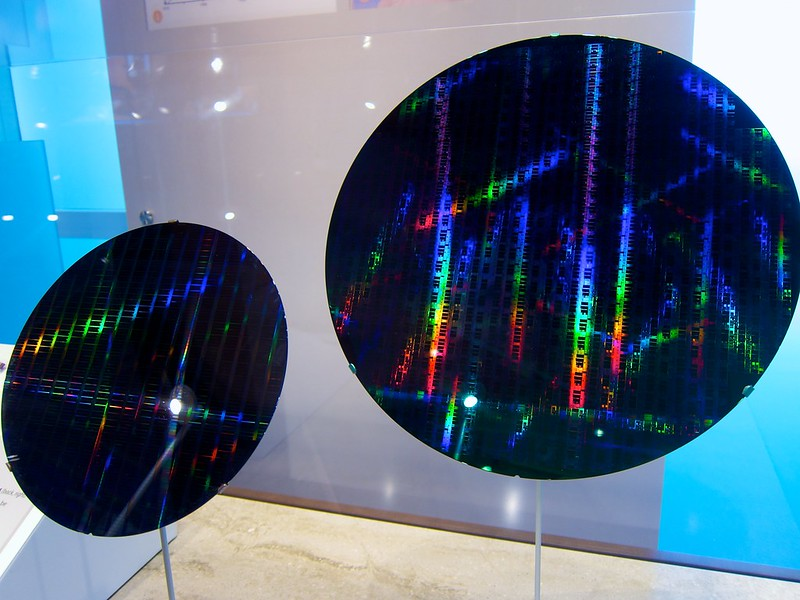
\includegraphics[width=0.5\textwidth]{silicon-wafers.jpg}
	\caption{Пластинки изрязани от силициев монокристал използвани за производството на компютърни чипове. \cite{debold_waffers_2011}}
	\label{fig:sillicon_wafers}
\end{figure}
Поради неделимата структура на градивните единици обаче следва, че няма как технологичният инструмент да среже ,,през атома``, т.е. получената повърхност при срязването на монокристала няма как да бъде гладка на атомно ниво, а се формират т.нар. \textit{стъпала}, a самата повърхност наричаме \textit{вицинална}.
\begin{figure}[htbp]
	\centering
	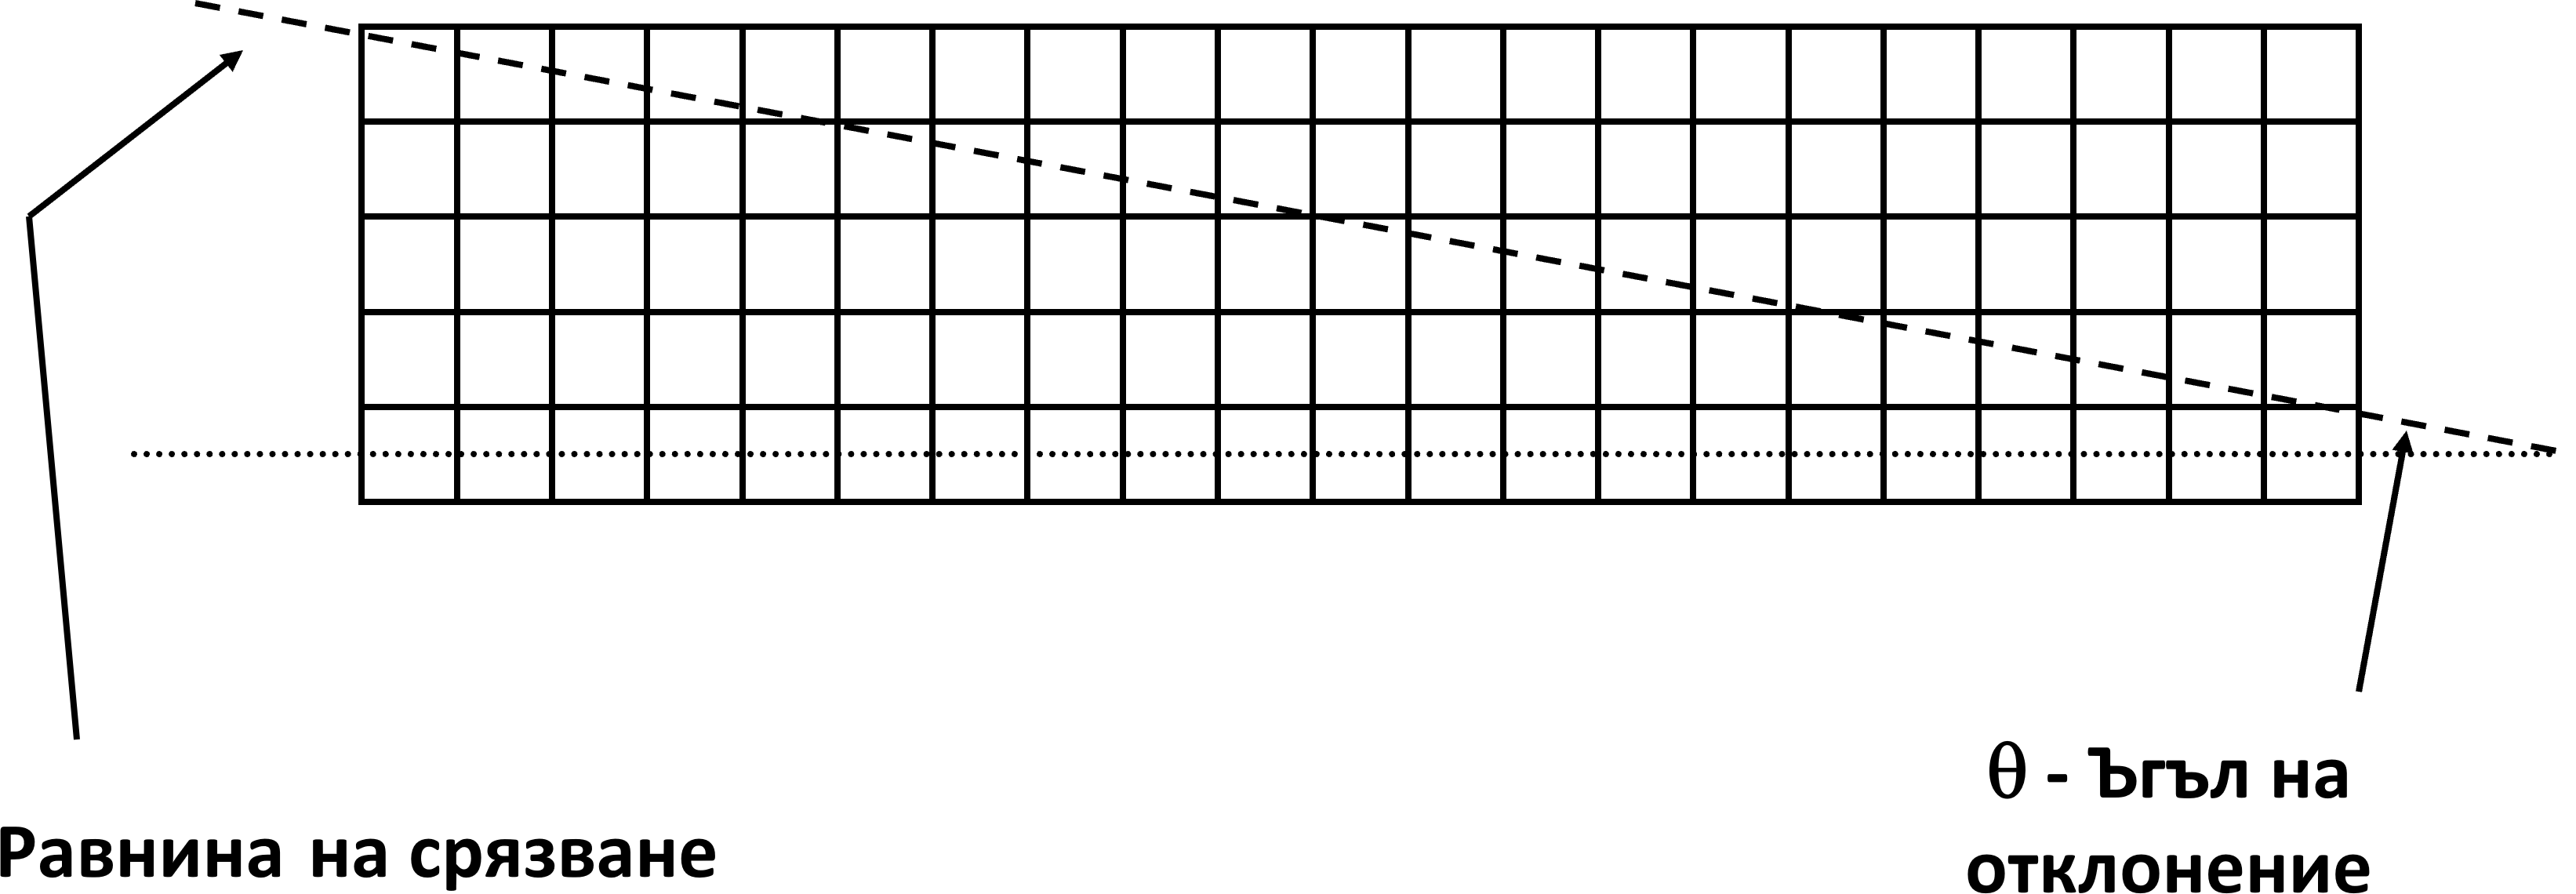
\includegraphics[width=\textwidth]{miscut.png}
	\caption{Схематично представяне на срязването на монокристал под ъгъл $\theta$}
	\label{fig:miscut_crystal}
\end{figure}

Ще различаваме между две основни структури, които са допълнителни на вициналната повърхност - тераси (непрекъснати части от повърхността с еднаква височина) и стъпала - преходите между две тераси. Ъгълът, под който е срязан монокристала дава началната ширина на терасите (разстояние между стъпалата) - $l_0$. Да обърнем внимание, че при постоянен ъгъл на срязване началното $l_0$ e еднакво за всички тераси. Такава вицинална повърхност с равномерно отдалечени стъпала ще бъде и началното условие за всички модели, които ще разгледаме.
\begin{figure}[htbp]
	\centering
	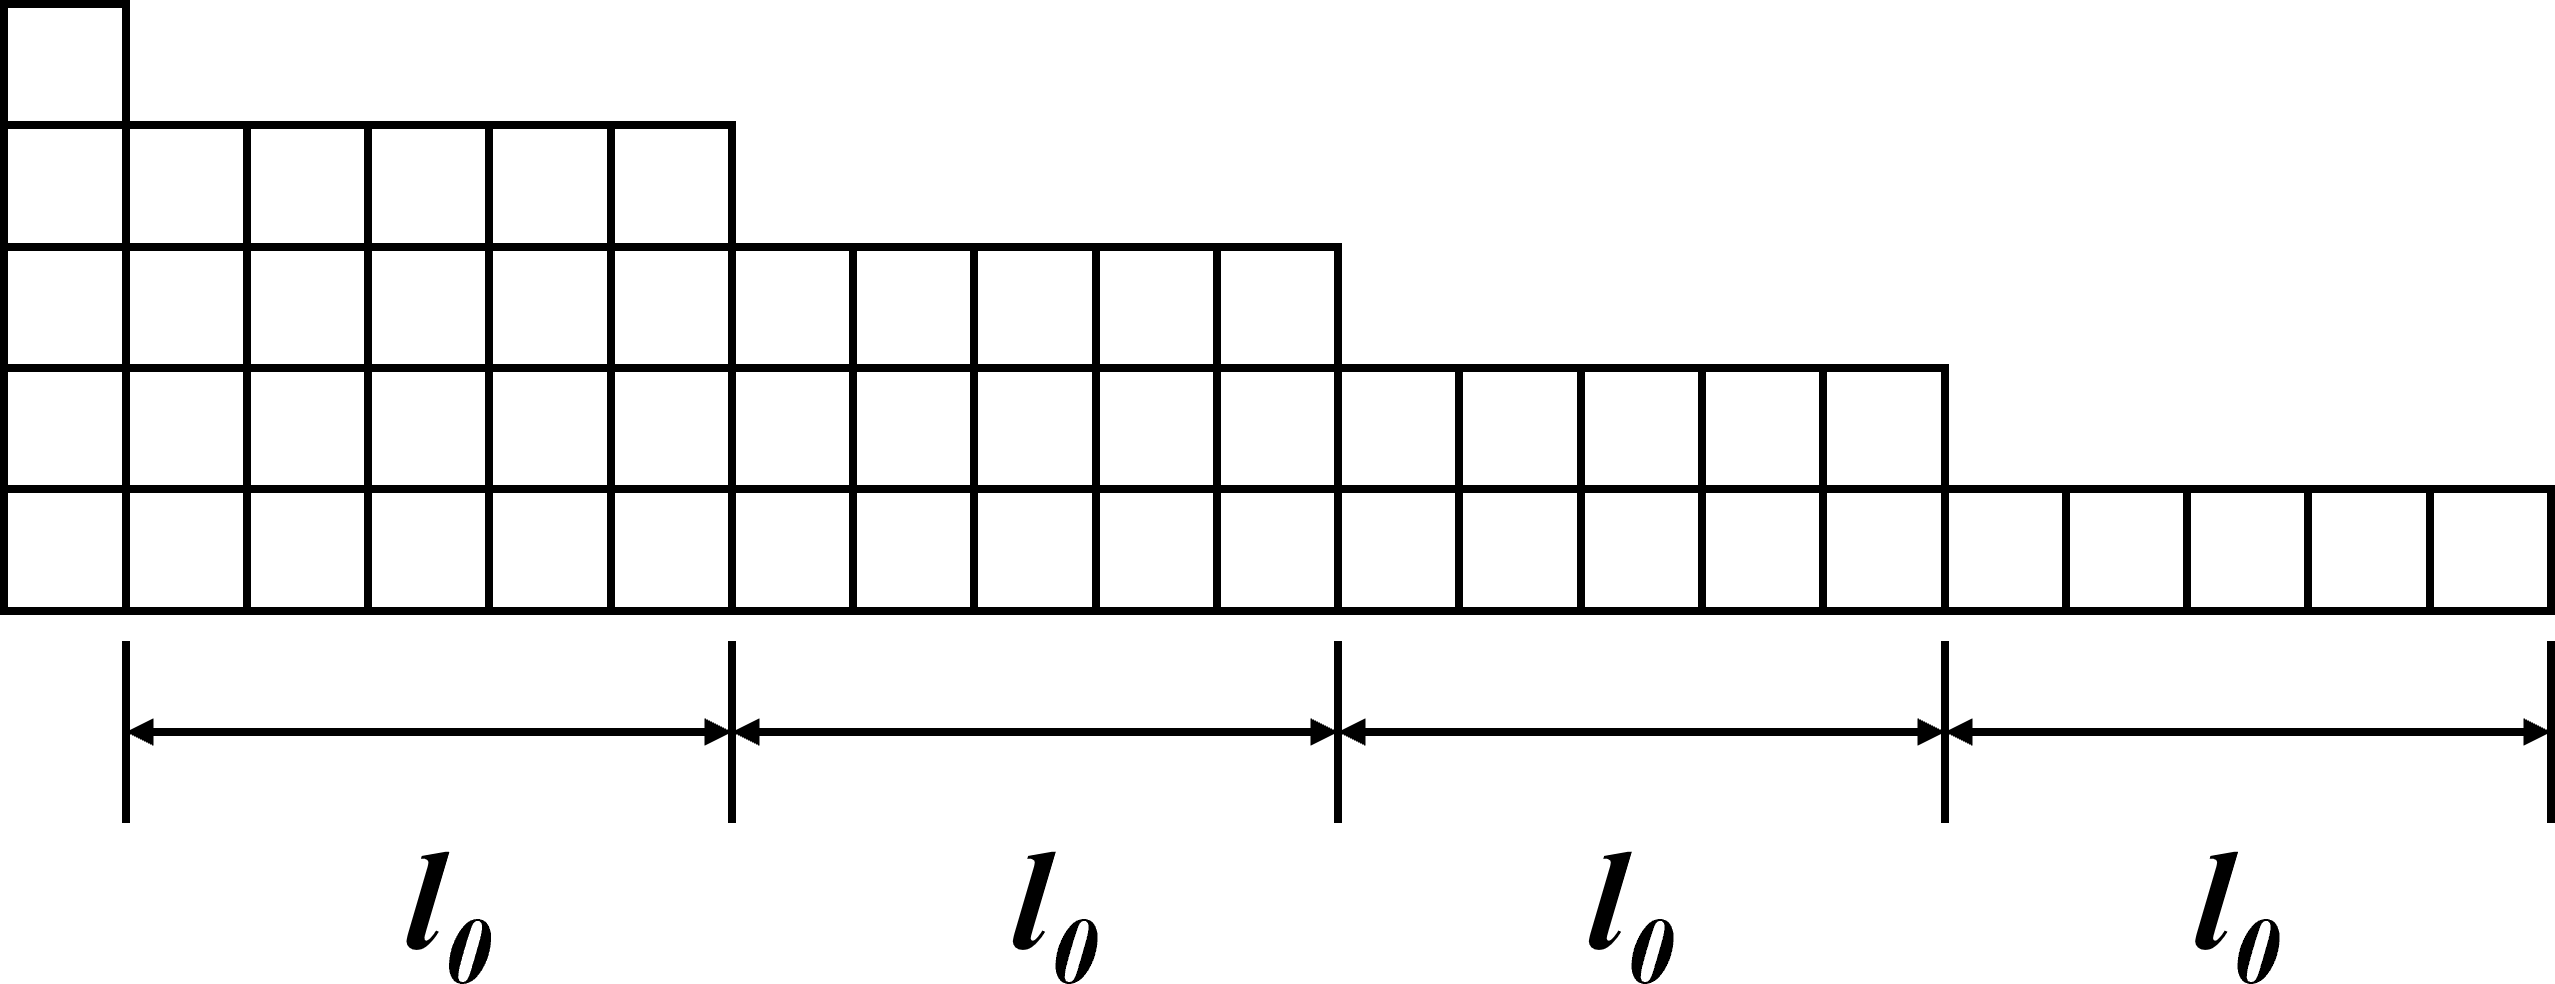
\includegraphics[width=\textwidth]{vicinal.png}
	\caption{Схематично представяне на вициналната повърхност. С $l_0  \propto \cot{\left( \theta \right)} $ e отбелязано началното вицинално разстояние между стъпалата (ширина на терасите).}
	\label{fig:initial_vicinal}
\end{figure}

\autoref{fig:miscut_crystal} и \autoref{fig:initial_vicinal} представят цялостния процес на формиране на една вицинална повърхност и ще служат като основа na следващите модели. Да обърнем внимание, че на една такава двумерна вицинална повърхност всяко от стъпалата всъщност представлява кинк-позиция. В 3D (вж. \autoref{fig:atoms_on_surface}) не е задължително всяка позиция на стъпало да бъде кинк позиция.
\subsection{Групиране на стъпалата (step bunching)}
През 1989~г. в статия от \textit{Latyshev et. al} \cite{Latyshev1989} е описано за пръв път т.нар. групиране на стъпала при растеж и/или сублимация (\textit{step bunching)} на кристалната повърхност на Si(111) в електрично поле. Започвайки от начална вицинална повърхност като показаната на \autoref{fig:initial_vicinal}, по време на процеса на растеж се наблюдава ефективно ,,придвижване`` на стъпалата по повърхността на растящия кристал, така че разстоянието между тях $l_{bunch}$ намалява спрямо началното вицинално разстояние $l_{bunch} < l_0$, като така се формират групи от стъпала на повърхността. Тези групи са разделени една от друга от тераси, чиято ширина е по-голяма от началната $l_{terrace}  > l_0$.
\begin{figure}[htbp]
	\centering
	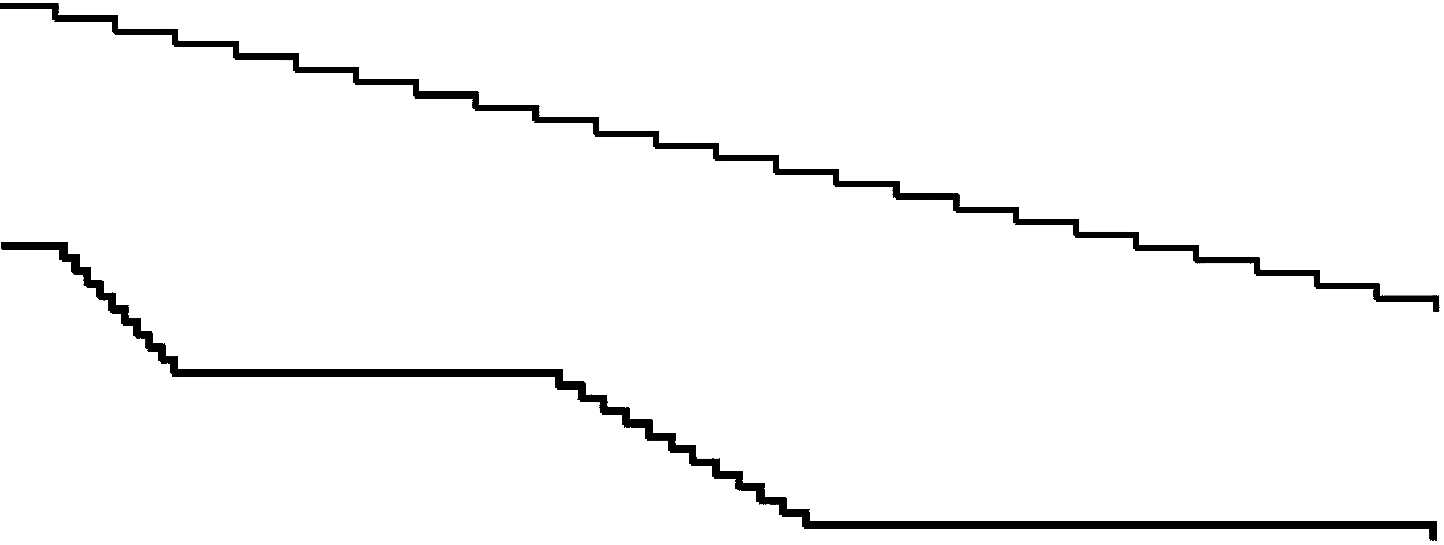
\includegraphics[width=\textwidth]{step_bunching_scheme.png}
	\caption{Схематично представяне на групиране на стъпалата върху кристалната повърхност. От начална вицинална повърхност с равни начални разстояния между стъпалата са формирани две групи в които $l_{bunch} < l_0$.}
	\label{fig:step_bunching}
\end{figure}
За да наблюдаваме такъв процес на реорганизация на повърхността, трябва в системата да съществува нестабилност, обуславяща движението на стъпалата едно спрямо друго. В литературата \cite{StoyanStoyanov1991}\cite{TonchevArxiv2012} са идентифицирани два основни източника на нестабилност при кристализация и изпарение - \textit{Ерхлих-Швьобелов ефект} (локален ефект) \cite{Ehrlich1966} \cite{Schwoebel1966} и електромиграция (обемен ефект) \cite{Latyshev1989}. Поради това в следващите параграфи ще разгледаме физиката зад тези два ефекта.
\subsubsection{Ерлих-Швьобелов (ЕШ) ефект}
Този ефект представлява представлява разлика в енергиите на свързването или отделянето на градивна единица към предната и задната тераса. Ефектът е локален и зависи от размера на терасите
отгоре и отдолу на стъпалото \cite{Krug2005}. Когато свързването е преференциално към предната тераса, ефектът се нарича \textit{нормален} (прав) Ерлих-Швьобелов ефект,  докато ако свърването е преференциално към задната - \textit{обратен} Ерлих-Швьобелов ефект. При растеж на метални кристални решетки е до голяма степен повсеместен нормалният ЕШ ефект, докато при полупроводници като Si(111) при високи температури се наблюдава обратния ЕШ, а при ниски - нормалният.
Този ефект води до нестабилност в системата - двете тераси, формиращи едно стъпало нарастват с различна скорост - това създава ефективно движение ,,напред`` на стъпалото и намаляване на разстоянието между стъпалата $l_{bunch} < l_0$.
\begin{figure}[htbp]
	\centering
	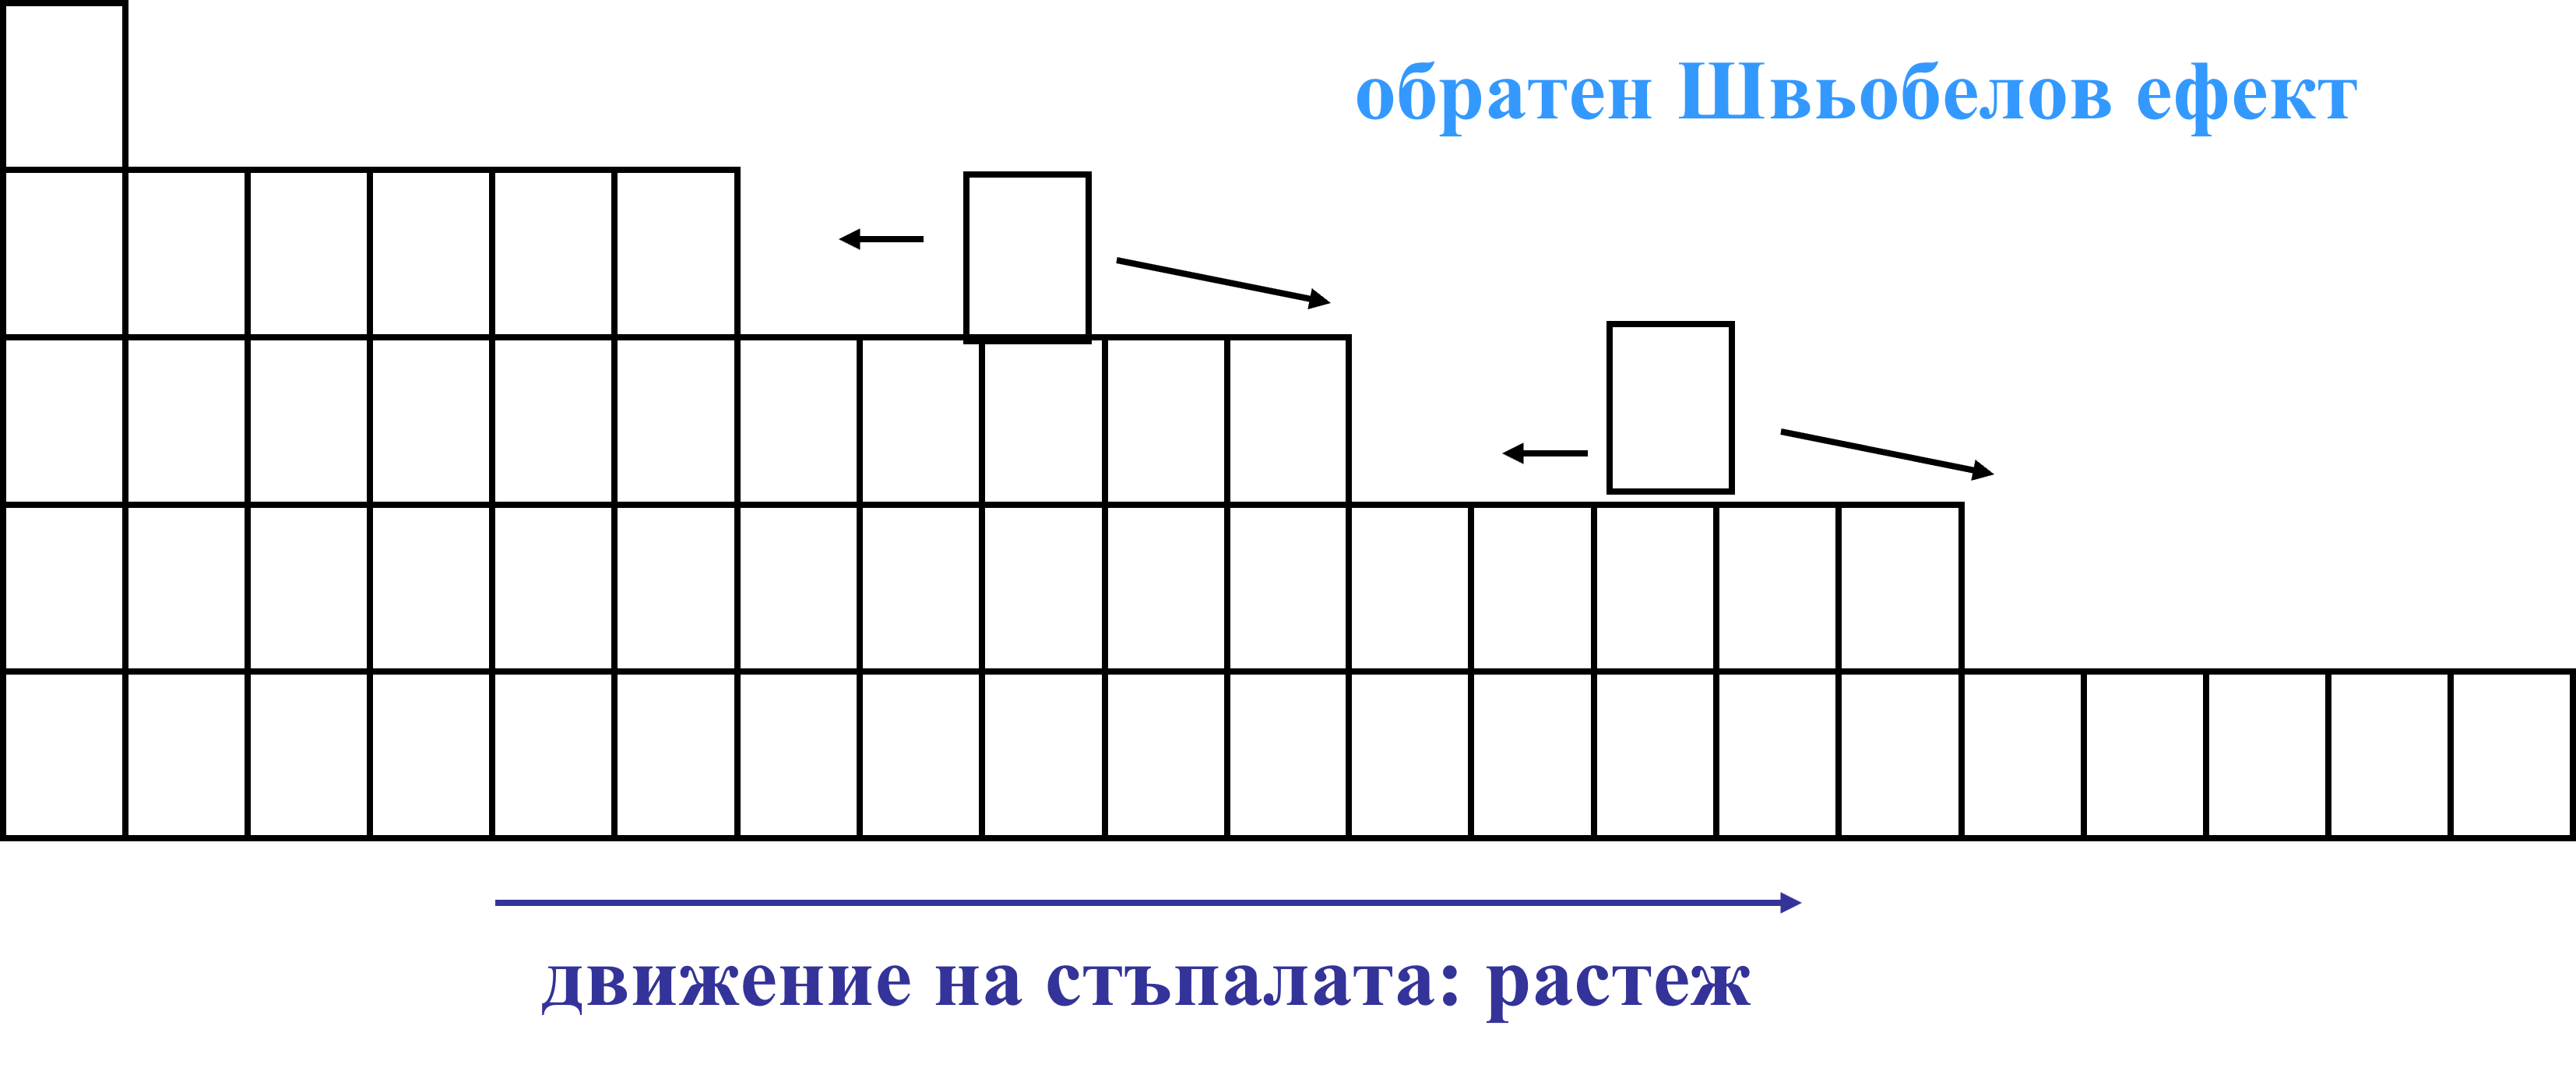
\includegraphics[width=\textwidth]{reverse_schwobel_effect_bunching.png}
	\caption{Обратен ЕШ ефект водещ до групиране на стъпалата при кристализация. Тук условно посоката на нарастване (кристализация) е взета да е надолу (надясно).}
	\label{fig:inverse_es_effect}
\end{figure}

На \autoref{fig:inverse_es_effect} e показано как обратният ЕШ при кристализация е ,,източник на нестабилност`` - задната тераса допринася повече към движението на стъпалото от предната (условно отбелязано с дължината на стрелките сочещи към съответната тераса). Съответно пертурбирайки задната тераса за $i$-тото стъпало напред (нараства с една градивна единица), това води до увеличаване на ефективната скорост на $i$-тото стъпало поради обратния ЕШ ефект. Пертурбирайки предната за $i$-тото стъпало тераса напред, тя се явява задна за $i+1$-вото стъпало и неговата скорост се увеличава. Обобщено, независимо към коя тераса се свърже градивната единица, обратния ЕШ е източник на нестабилност при кристализация.
\begin{figure}[htbp]
	\centering
	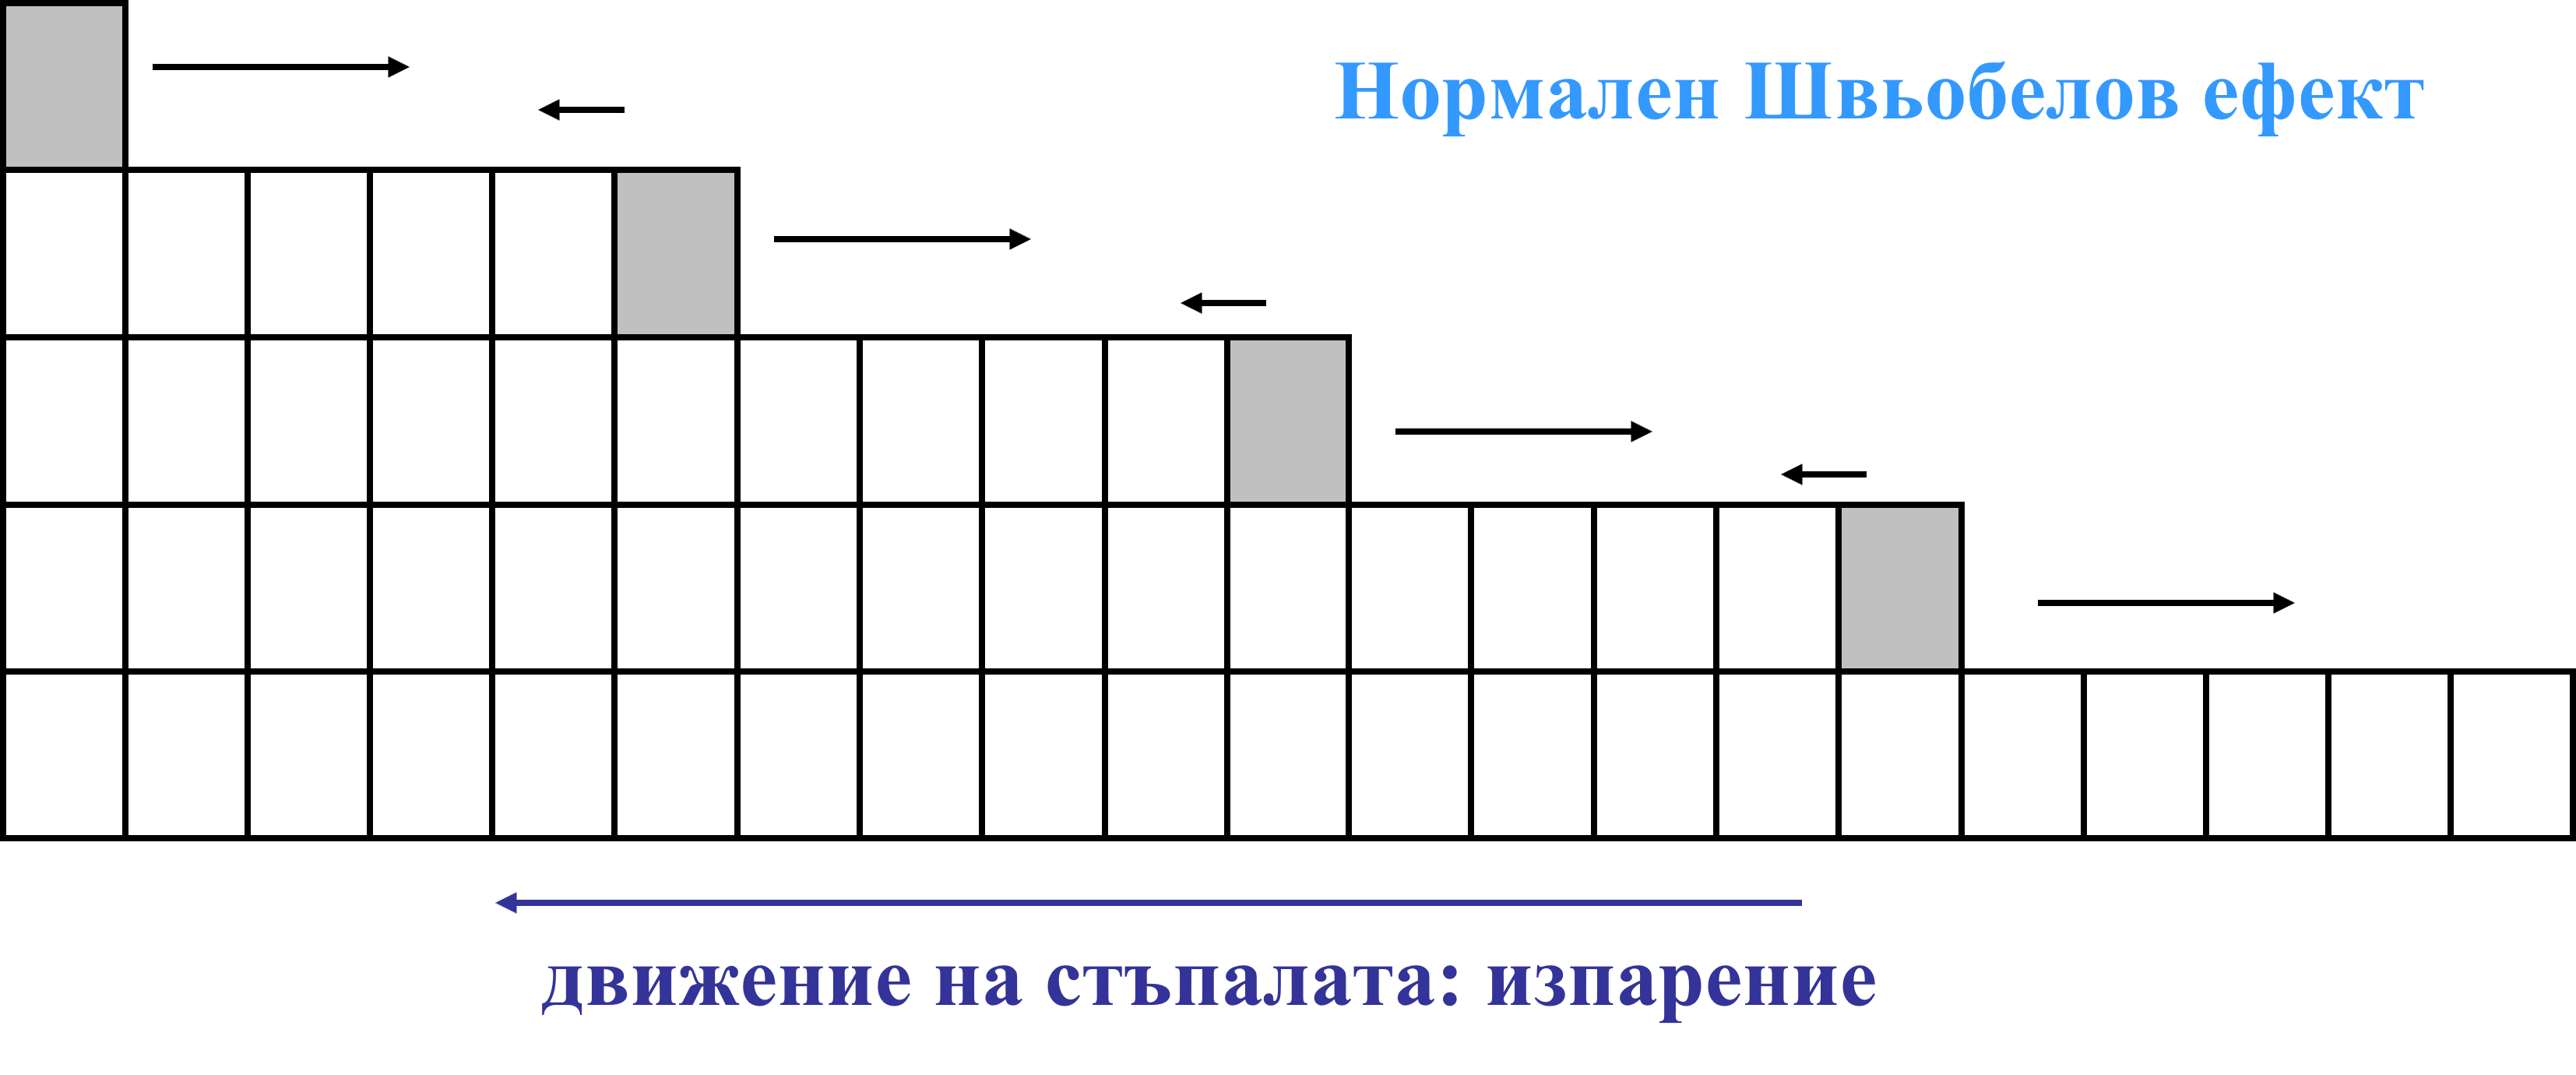
\includegraphics[width=\textwidth]{normal_schowbel_effect.png}
	\caption{Нормален ЕШ ефект водещ до групиране на стъпалата при изпарение. Тук условно посоката на изпарение (сублимация) е взета наляво (нагоре).}
	\label{fig:normal_es_effect}
\end{figure}

\autoref{fig:normal_es_effect} показва обратния на кристализацията случай - изпарението, тук нормалният ЕШ ефект действа в обратна посока (нагоре). Чрез аналогични разсъждения за пертурбиране на стъпалата може да се покаже, че нормалният ЕШ е източник на нестабилност при изпарение. Тук различното е, че градивните единици ще се откъсват от съответната им тераса.

ЕШ е \textbf{локален ефект}, който води до нестабилност в системата. За него най-важното е, че той е насочен нагоре или надолу по терасите в зависимост от това дали разглеждаме кристализация или сублимация.  В случая, когато имаме нормален ЕШ при растеж се наблюдава друг интересен режим на нестабилност на вициналната повърхност - меандриране. Меандрирането също е особен ефект и изисква собствено изучаване, което не е цел на настоящия труд. \cite{Krug2005} Следващият ефект, който ще разгледаме - \textit{електромиграцията}, насочена в една и съща посока тя е източник на нестабилност и за растеж, и за изпарение.

\subsubsection{Електромиграция}
Електромиграцията е процес на пренос на заредени частици под действието на електрично поле. В контекста на кристализация и по-конкретно - групиране на стъпала, електричното поле създава насочено движение (адвекция) на градивни частици по посока на нарастване на потенциала.
За разлика от нормалния и обратния ЕШ ефект, елеткромиграцията е \textit{обемен} ефект - това означава, че силата, която действа на атомите се характеризира изцяло с векторното поле на електричния потенциал $\overline{f}$ и не зависи от размера на съседните на $i$-тото стъпало тераси. Допълнително - електромиграцията е източник на нестабилност и води до съответно групиране на стъпалата при една и съща посока на силата (напр. надолу) за случаите на кристализация и сублимация.

\autoref{fig:electromigration_crystalization} и \autoref{fig:electromigration_sublimation} илюстрират поведението на системата при нестабилност вследствие електромиграция. Електричното поле води до преференциално свързване към задната на $i$-тото стъпало тераса при групиране и отделяне от предната за $i$-тата тераса при сублимация, така резултатът и в двата случая е групиране на стъпалата при еднаква посока на силата.
\begin{figure}[htbp]
	\centering
	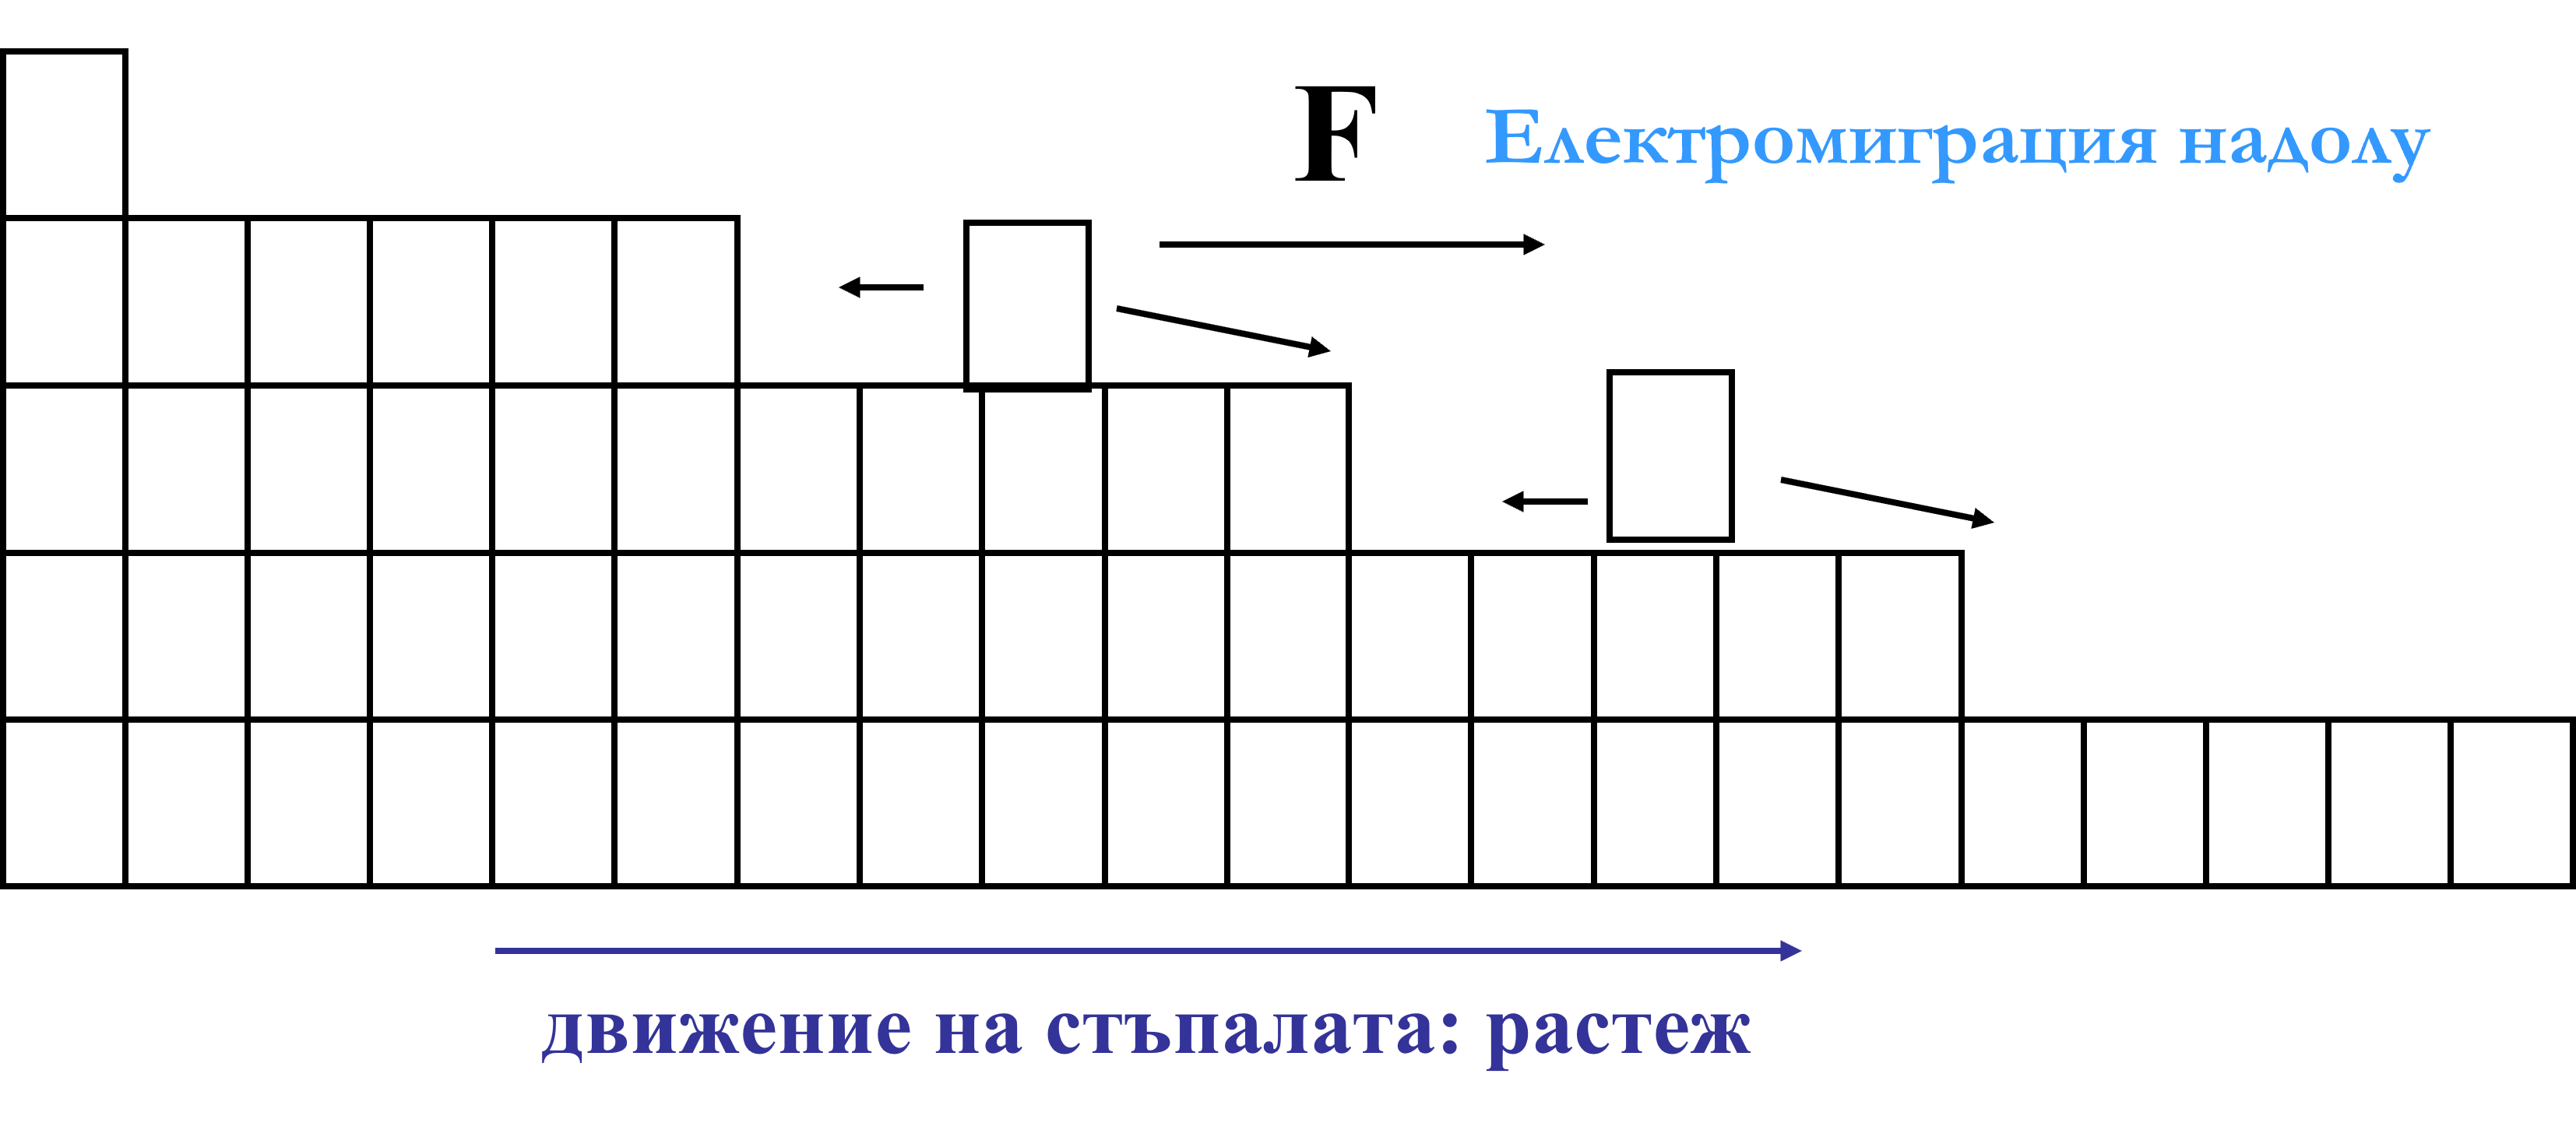
\includegraphics[width=\textwidth]{electromigration_growth.png}
	\caption{Електромиграция насочена условно надолу при кристализация, водеща до преференциално свързване към задната тераса и групиране.}
	\label{fig:electromigration_crystalization}
\end{figure}
\begin{figure}[htbp]
	\centering
	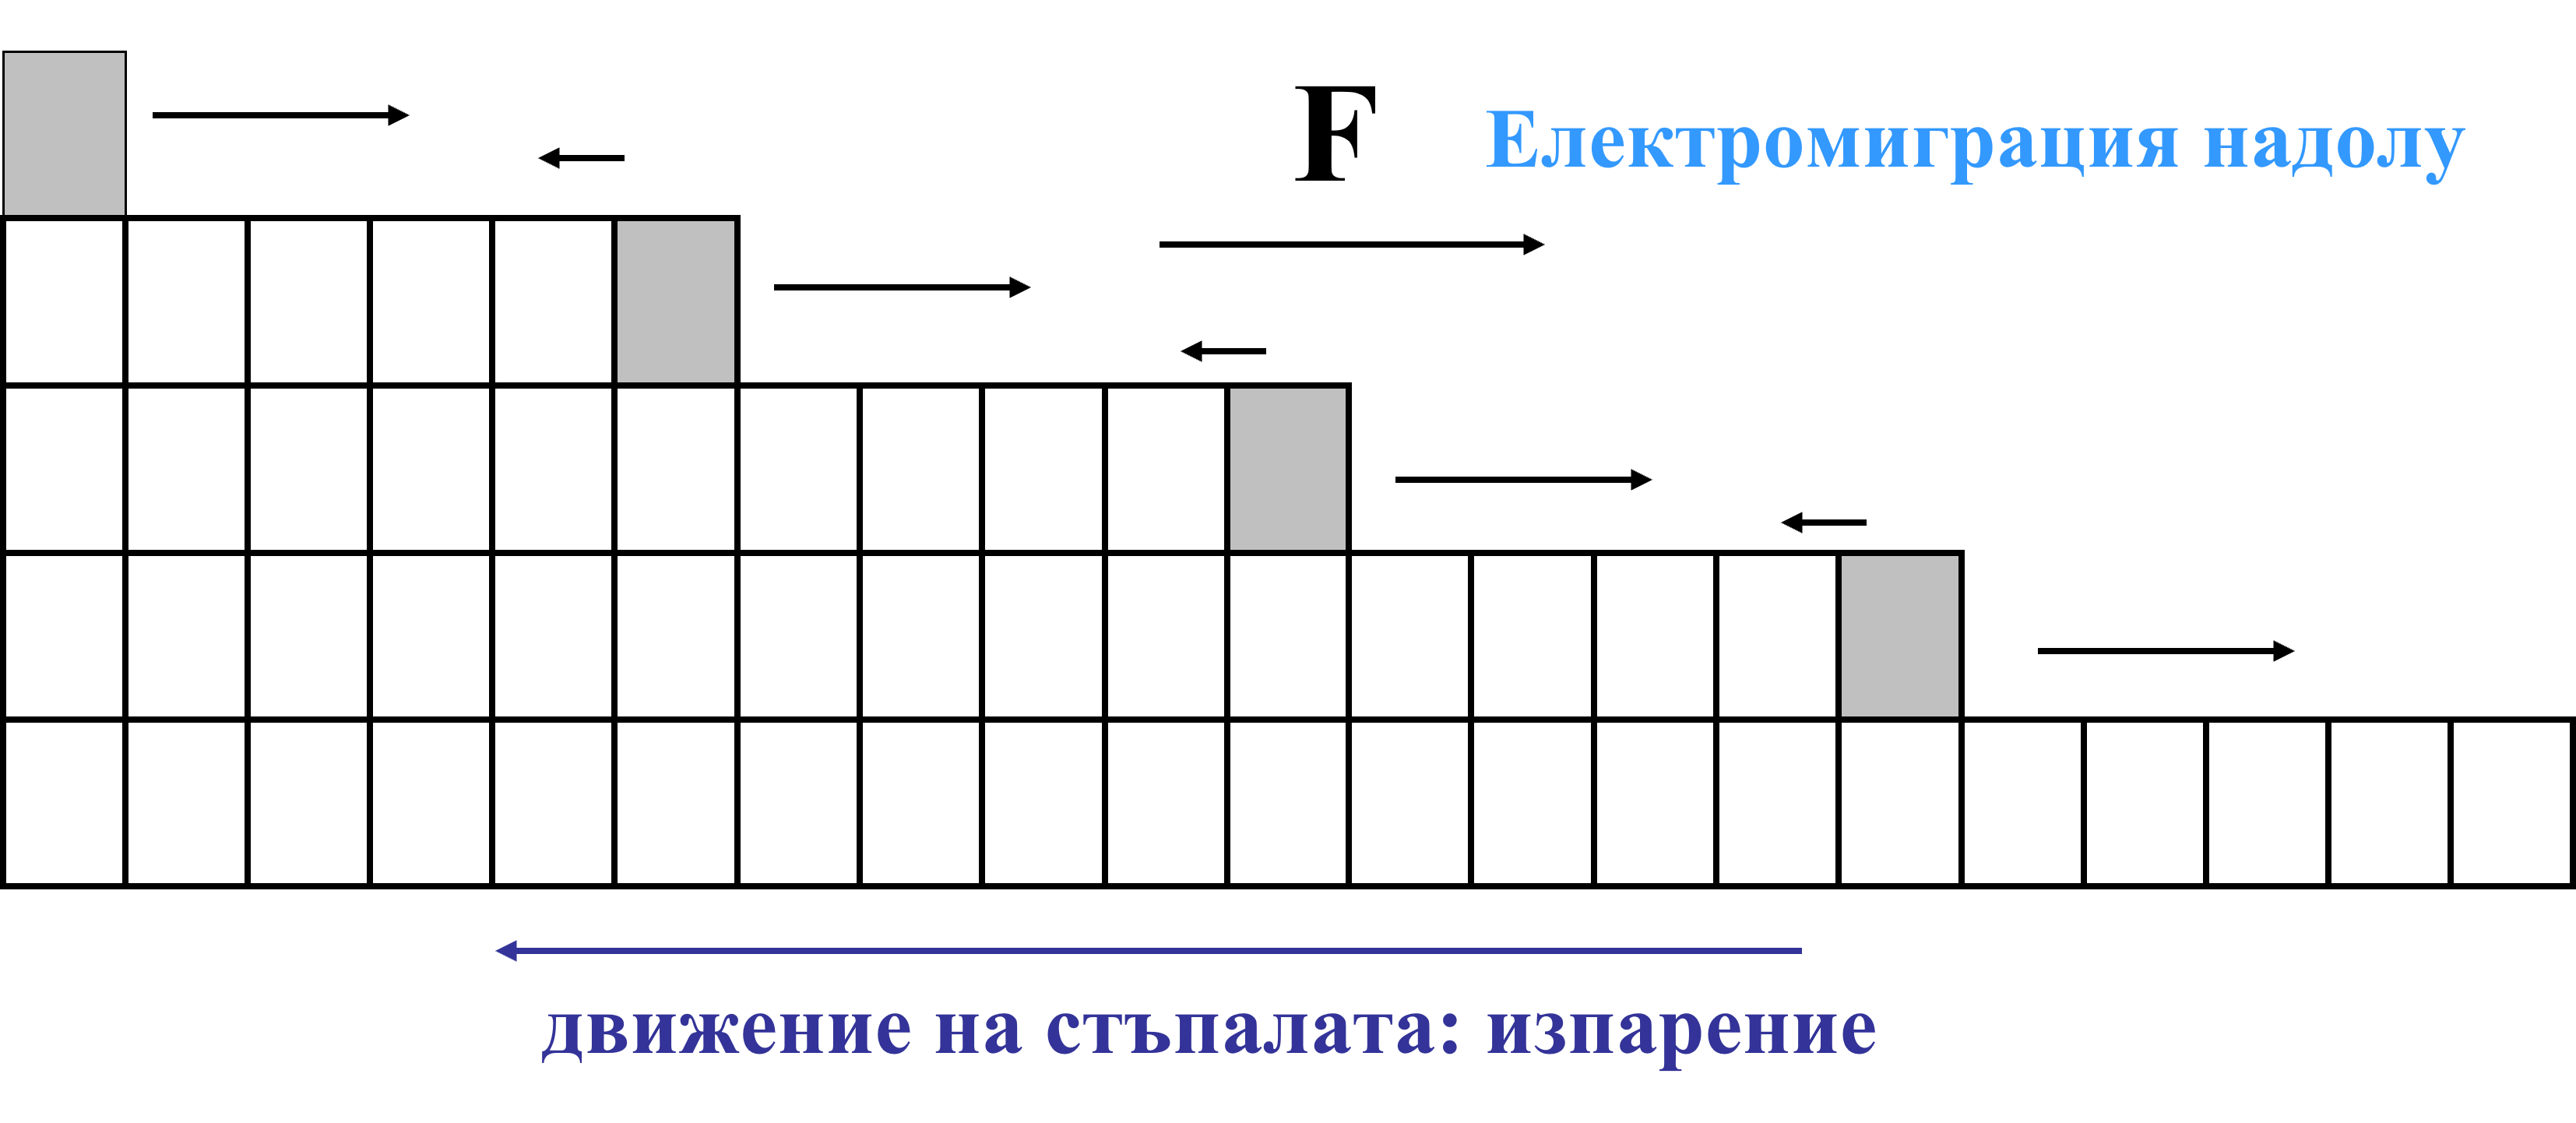
\includegraphics[width=\textwidth]{electromigration_sublimation.png}
	\caption{Електромиграция насочена условно надолу при сублимация, водеща до преференциално отделяне от предната тераса и групиране.}
	\label{fig:electromigration_sublimation}
\end{figure}

\subsection{Динамика на адатомите}
Динамиката на стъпалата може да се разглежда като задача с подвижна граница (moving boundary problem), като самото стъпало е идеализирана математическа граница между две съседни тераси (скок във функцията описваща локалната височина на повърхността), която еволюира чрез обмен \textit{през} непрекъснатото поле на адатомите в околността на повърхността $N(\overline{x}, t)$. $N$ - брой адатоми в полето, $\overline{x}$ - координата в пространството над повърхността, $t$ - време. \cite{Krug2005} Ще разгледаме модел на групиране под електромиграция, тъй като обемният характер на силата прави този случай по-прост.
Нека отбележим с $D = const$ - дифузионния коефициент на адатомите, $k_B$ - болцманова константа, $Т$ - абсолютна температура, $\overline{f}$ - сила на електромиграция, $G$ - поток на отлагане на адатомите, $\tau$ - характеристично време на отлагане. Комбинирани тези ефекти дават за еволюцията на адатомното поле:
\begin{equation}
	\label{eq:advection_diffusion_adatom_dynamics}
	\frac{\partial N}{\partial t} = D \nabla^2 N - \frac{D}{k_B T} \overline{f} \cdot \nabla N + G - \frac{N}{\tau} = - \nabla \cdot J + G - \frac{N}{\tau}
\end{equation}
\autoref{eq:advection_diffusion_adatom_dynamics} e уравнение от вида адвекция-дифузия. Обобщеният поток на адатомите тогава е:
\begin{equation*}
	J = -D \nabla N + \frac{D}{k_{B} T} \overline{f} N
\end{equation*}
\begin{equation*}
	\nabla \cdot \overline{f} = 0
\end{equation*}
Коефициентът $D/(k_{B} T)$ се нарича подвижност на адатомите. 

Докато самото ЧДУ е стандартно от математическа гледна точка, особени са граничните условия върху стъпалата. Те са условия на Робин за локалния поток върху границите на терасата. Нека $j_+$ е локалният поток върху отляво на терасата (прииждащ по посоката на кристализация), а $j_-$ е този отдясно (напускащ). Обикновено те са рескалирани спрямо локалния равновесен брой адатоми:
\begin{align*}
	j_+ &= k_+ (N_+ - N_{eq}) + p (N_+ - N_{eq}) \\
	j_- &= k_- (N_- - N_{eq}) + p (N_- - N_{eq}) 
\end{align*}
Където $k_+$ и $k_-$ са склонностите за свързване към двете стъпала, а $p$ e т.нар. \textit{прозрачност} на стъпалото. Тогава, на база закона за материалния баланс в система, получаваме следните г.у. за потоците $j_+$ и $j_-$.

\begin{align*}
	j_+  &= D \overline{n} \left[ \nabla N|_+ - \frac{1}{k_B T} \overline{f} N \right] \\
	j_-  &= - D \overline{n} \left[ \nabla N|_- - \frac{1}{k_B T} \overline{f} N \right] 
\end{align*}
Където $\overline{n}$ е единичната нормала към стъпалото, която сочи към долната тераса, а  $N|_\pm$ са броя адатоми от двете страни на стъпалото \cite{Krug2005}.
\textit{Стоянов} \cite{StoyanStoyanov1991} решава \autoref{eq:advection_diffusion_adatom_dynamics} в едномерния (1D+t) случай и показва, че когато електромиграцията е насочена надолу по стъпалата (по посока на кристализацията), действително се наблюдава групиране в този модел. 

Подвижните гранични условия в тази задача я правят значително сложна дори за числено изследване в по-голям брой измерения - 2D + t, 3D + t. 

Затова за 1D+t случая може да се направи значително опростяване като повърхността се сведе до едномерна такава, като в началото на всяка позиция $X_i, i = \overline{1,N}$ имаме стъпало. Така ще получим един окрупнен модел под формата на ОДУ, в който стъпалата от \autoref{fig:step_bunching} са заместени с точки (техните позиции) върху числова ос.

\subsection{ОДУ модел за скоростта на стъпалата}
\begin{figure}[htbp]
	\centering
	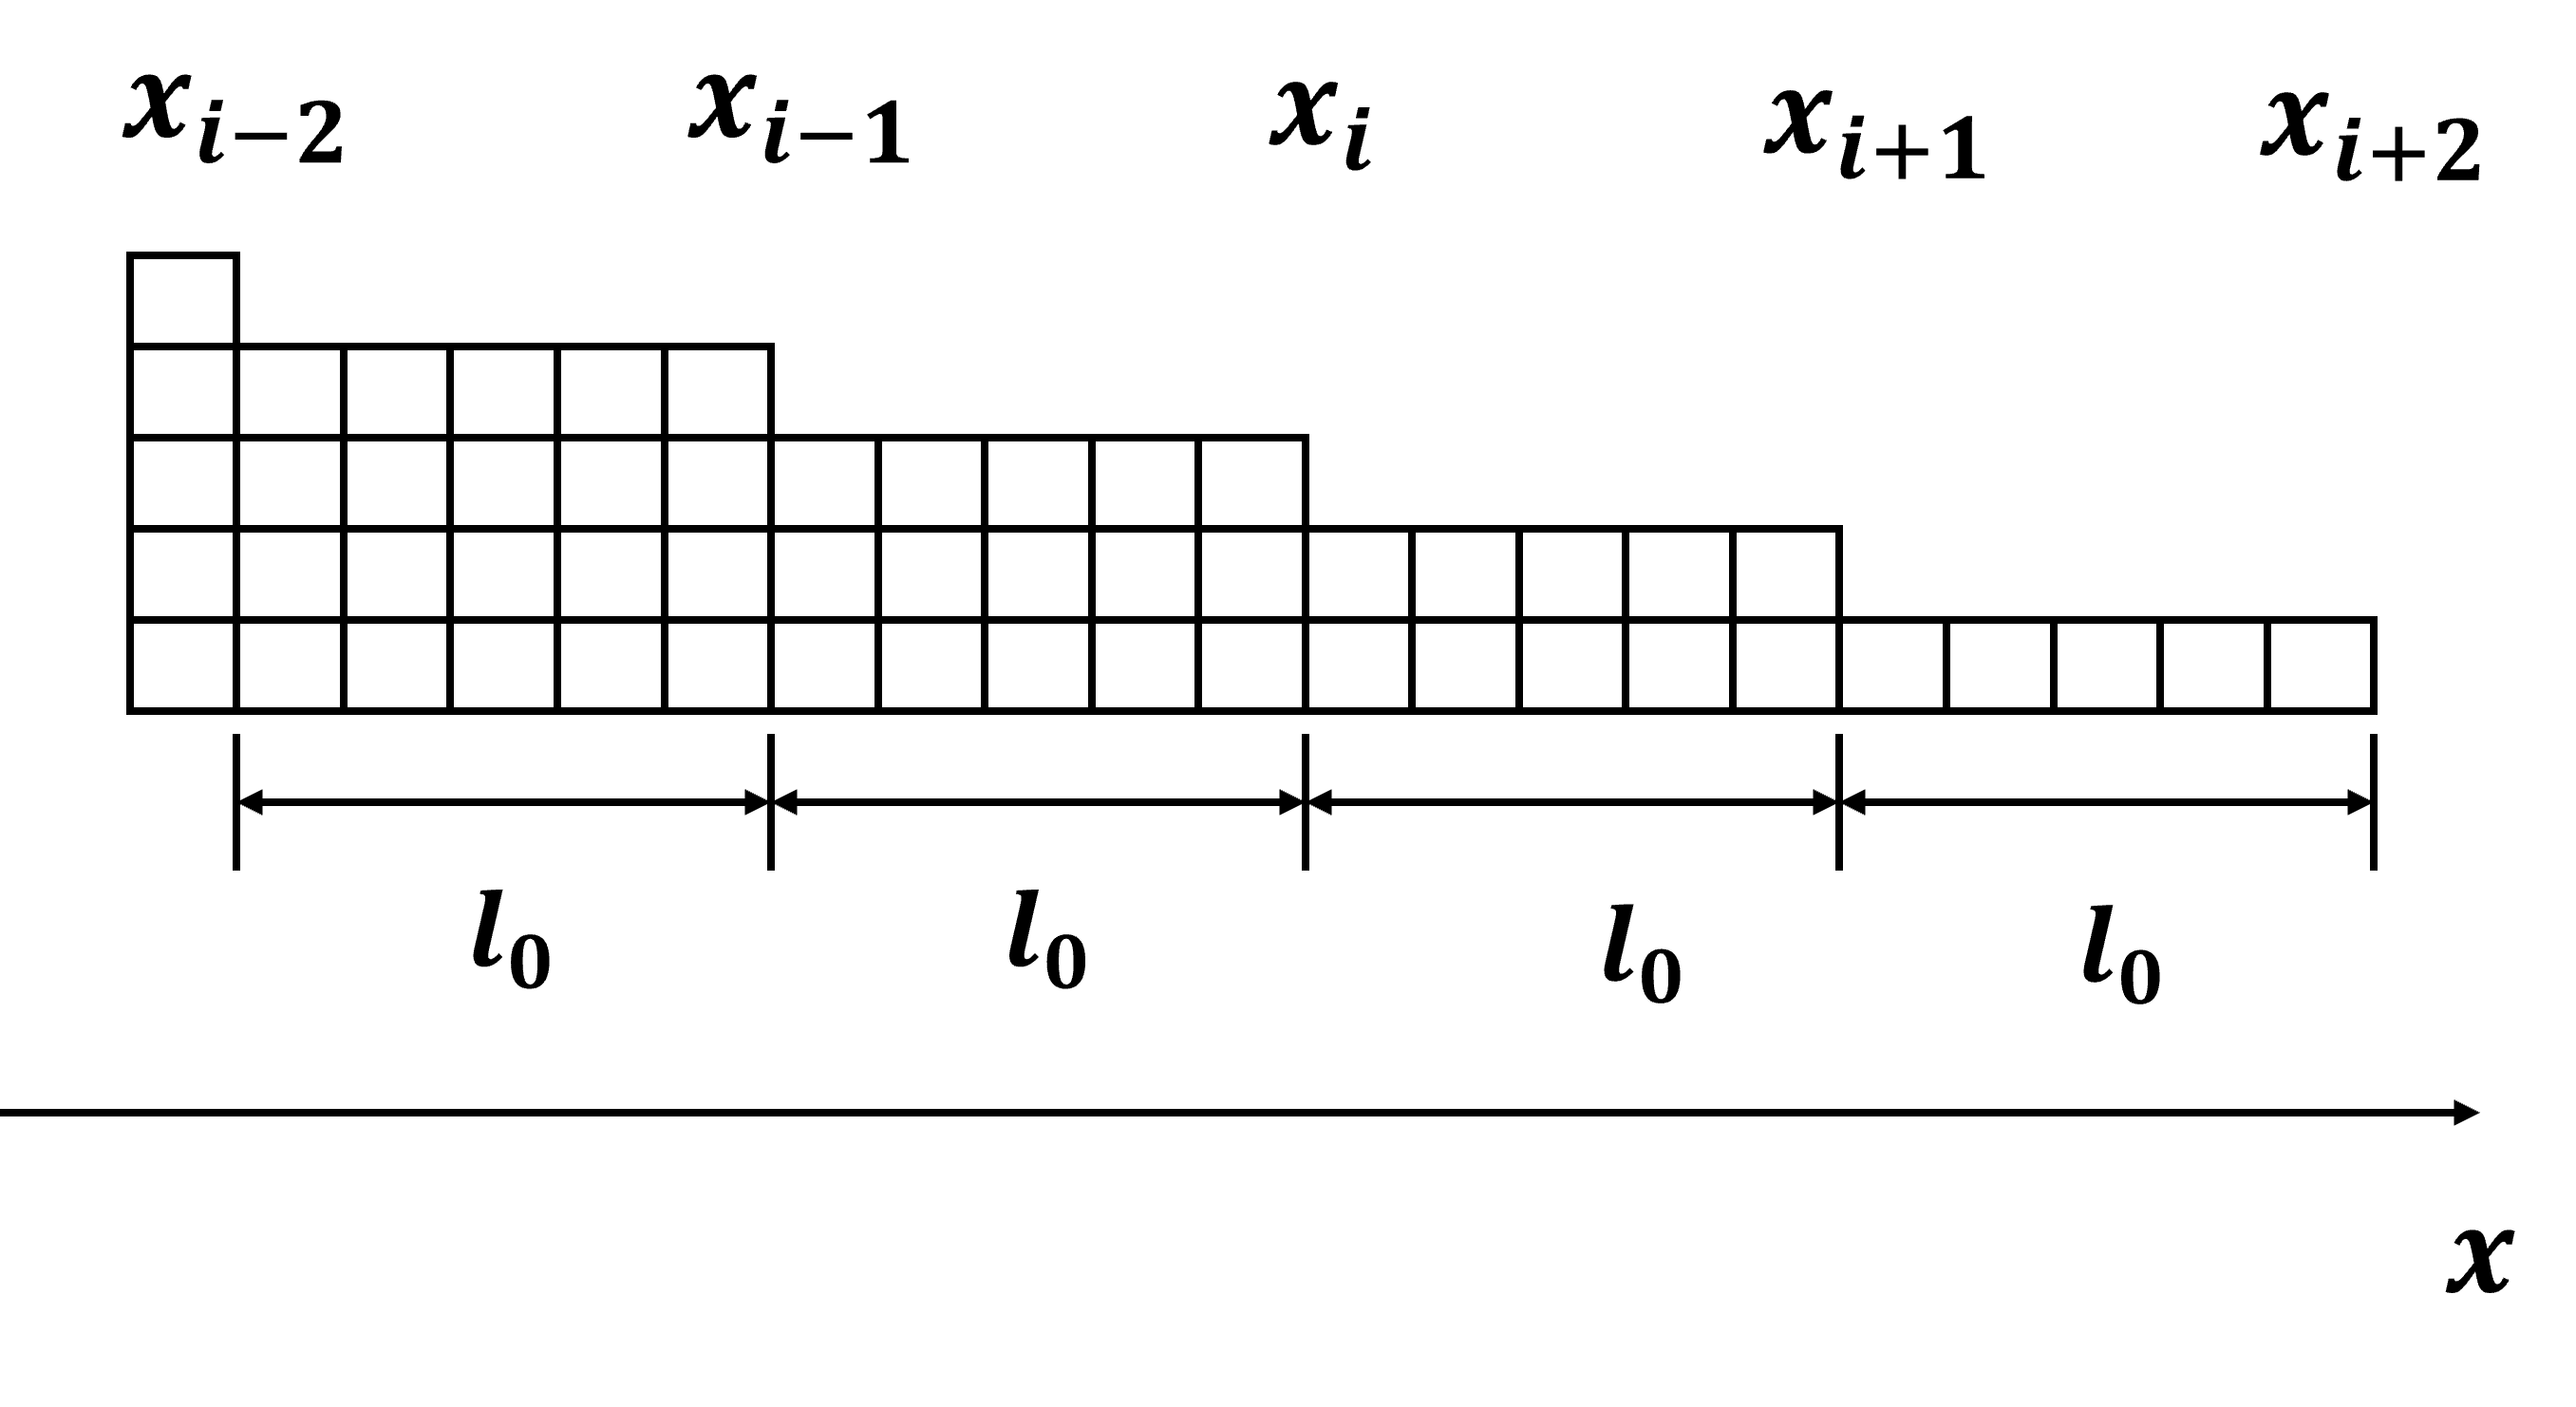
\includegraphics[width=\textwidth]{step_growth_direction.png}
	\caption{Схематично представяне на модела. За положителна посока по $x$-приемаме посоката ,,надолу`` по стъпалата. С $x_{i}, i = \overline{1, N}$ означаваме позициите на съответните стъпала.}
	\label{fig:step_growth_ode_model_scheme}
\end{figure}
Нека спрямо \autoref{fig:step_growth_ode_model_scheme} да приемем, че на всяка позиция $x_{i}$ имаме стъпало. Разликата във височината между всяко стъпало да е една градивна единица и в началото, те да са на равно разстояние едно от друго $l_0$ - началното вицинално разстояние. Допълнително, нека:
\begin{equation*}
    \Delta x_i \coloneqq x_i - x_{i - 1}
\end{equation*}
Това e ширината на $i$-тата тераса - тази за която $i$-то стъпало е долното такова.
Тогава за скоростта на $i$-тото стъпало можем да запишем в най-общ вид ОДУ, чието н.у. е началната вицинала с периодични г.у. (първото стъпало \textbf{е до} N-тото) \cite{Krasteva2016}:
\begin{equation}
    \frac{d x_i}{d t} = k a_i + u r_i
    \label{eq:general_step_velocity_ode}
\end{equation}
Където с $a_i$ сме обозначили функция на $\Delta x_{i-n}, \Delta x_{i-n + 1}, ..., \Delta x_{i}, ... \Delta x_{i + n} $ отчитаща обобщено силите на привличане, а с $r_{i}$ - функция на  $\Delta x_{i-n}, \Delta x_{i-n + 1}, ..., \Delta x_{i}, ... \Delta x_{i + n}$ (големината на $n$-те задни и $n$-те предни тераси) - отчитаща силите на отблъскване. В общия случая се разглеждат до първи и втори съседи $n = 0,1$. Параметрите $k$ и $u$ са константите на пропорционалност между двете сили (безразмерни). Конкретни изрази за $a_i, r_i$ ще бъдат дадени по-нататък. 

\subsubsection{Автомоделни решения}
Искаме да намерим автомоделни решения \cite{Barenblatt1996} \cite{Krasteva2016}:
\begin{equation}
    t^\delta l = s_{l t} 
    \label{eq:dimensional_scaling}
\end{equation}

Където $l(t)$ e характеристично за групите разстояние (напр. $l_{min}$ - минимално разстояние в дадена група),  $s_{l t} = f(k, u, l_0)$ е автомоделната функция. Тя следва да е функция на параметрите на модела $k, u$ и началното разстояние $l_0 = l_{min} (0)$. Тук $\delta$ е времевата експонента на динамичния скейлинг и e безразмерна величина \cite{Vicsek1984}. Такива автомоделни решения описват самоподобието на групите, които се формират:
\begin{equation*}
    l(t_1) t_1^\delta = l(t_2) t_2^\delta
\end{equation*}
Записано във вида \autoref{eq:dimensional_scaling} показва, че за размерността на автомоделната функция имаме:
\begin{equation*}
    \left[s_{l t} \right] = T^\delta L
\end{equation*}
Където T, L са съответно размерностите за време и дължина. За да отговаря на анзаца на \textit{Family-Visceck}, искаме да обезразмерим това уравнение и да получим скейлинговата функция в ,,чист вид``. За целта ще започнем с обезразмеряването на \autoref{eq:general_step_velocity_ode}.
Ще дефинираме безразмерното разстояние и време съответно:
\begin{align*}
    X_{i} & \coloneqq \frac{x_i}{\xi_0} \\
    T & \coloneqq \frac{t}{\tau_0}
\end{align*}
Тук обезразмеряванията и скалите $\xi_0, \tau_0$ са въведени естествено, без ограничение на общността на уравнението.
Ще направим \textit{допускането} че $[a_i] = L ^ \nu $ и $[r_i] = L ^ \mu$, т.е. в размерността им единствено участва дължината. Това означава, че тези сили на привличане и отблъскване зависят от времето единствено чрез размера на терасите в дадения момент, което не е силно ограничение в общността и е физически обосновано допускане (кохерентност на групите). Тогава дефинираме безразмерните сили на взаимодействие:
\begin{align*}
    A_{i} & \coloneqq \frac{a_i}{\xi_{0}^ \nu} \\
    R_{i} & \coloneqq \frac{r_i}{\xi_{0}^ \mu}
\end{align*}
Заместваме и получаваме:
\begin{equation*}
    \frac{\xi_0}{\tau_0} \frac{d X_i}{d T} = \xi_0^\nu k A_i + \xi_0^\mu u R_i
\end{equation*}
\begin{equation*}
    \frac{d X }{d T} = \tau_0 \xi_0^{\nu-1} k A_i + \tau_0 \xi_0^{\mu-1} u R_i
\end{equation*}
Тъй като досега не сме допуснали нищо за $\tau_0, \xi_0$ ще ги изберем така, че в основното ОДУ да няма експлицитно параметри. Така имаме системата от уравнения за скалите:
\begin{equation}
    \begin{cases}
        \tau_0 \xi_0^{\nu-1} k = 1 \\
         \tau_0 \xi_0^{\mu-1} u = 1
    \end{cases} 
\end{equation}
Решаваме системата за скалите и получаваме:
\begin{align*}
    \xi_0 &= \left( \frac{u}{k} \right)^ {\frac{1}{\nu - \mu}} \\
    \tau_0 &= k^{-1} \left( \frac{u}{k} \right) ^ {\frac{1-\nu}{\mu - \nu}}
\end{align*}
И обезразмерено диференциалното уравнение:
\begin{result}{Oбезразмерен общ ОДУ модел на групиране}{ode_general}
    \begin{equation}
        \label{eq:non_dimenisonal_ode}
        \frac{d X_i}{d T} = A_i + R_i
    \end{equation}
\end{result}
С обезразмерено начално разстояние: $L_0 \coloneqq \frac{l_0}{\xi_0}$.
Можем сега да получим и безразмерната форма на \autoref{eq:dimensional_scaling}.
\begin{align*}
    l t^\delta &= s_{l t}(l_0, k, u) \\
    \frac{l}{\xi_0} \left(\frac{t}{\tau_0}\right)^{\delta} &= L T ^\delta = S_{L T} (L_0)
\end{align*}
Където $L \coloneqq \frac{l}{\xi_0}$, $T \coloneqq \frac{t}{\tau_0}$. Заместваме скалите, извършваме алгебричните преобразования и получаваме \cite{Krasteva2016}:
\begin{equation*}
    l t ^ \delta =  \left( \frac{u}{k} \right)^ {\frac{1}{\nu - \mu}} k^{-\delta} \left( \frac{u}{k} \right) ^ {\delta \frac{1-\nu}{\mu - \nu}} S_{L T} (L_0)
\end{equation*}
Където $S_{L T}$ е безразмерната автомоделна функция, която зависи \textbf{само} от обезразмереното начално разстояние $L_0$.

С проведената процедура по обезразмеряване на задачата постигнахме следното:
\begin{itemize}
    \item Намерихме ,,естествените`` скали на задачата.
    \item В основното ОДУ нямаме параметри.
    \item Намалихме параметрично пространство от $(k, u, l_0)$ на едномерното - $(L_0)$.
    \item Получихме автомоделна функция $S_{L T}$, която зависи \textit{само} от началното разстояние $L_0$.
\end{itemize}

Освен аналитичните резултати как влияят параметрите на модела върху решения от вида на \autoref{eq:dimensional_scaling}, това обезразмеряване значително намалява необходимите изчисления за числено изследване на модела при различен конкретен вид на привличането и отблъскването на стъпалата. Ако в размерната версия например правим по 10 ,,експериментални резултата`` за всеки параметър, то общо ще са ни необходими 1000 числени експеримента, при безразмерния модел - само 10, т.е. сложността на задачата е намалена от $O(n^3)$ до $O(n)$.

\subsubsection{Изрази за силите на привличане и отблъскване}
Във времето са разработени разнообразни ОДУ модели в литературата по групиране, които отговарят на общия вид зададен от \autoref{eq:non_dimenisonal_ode}. Те обикновено са публикувани в размерена форма и параметрите $k, u$ в тях могат да имат сложен ви. Най-важното за всеки от тях е, че $k, u$ не зависят от размера на терасите. Те например могат да носят зависимостта от температурата, да отчитат материалните характеристики на повърхността и т.н.

Ще разгледаме безразмерните форми на моделите на \textit{Liu \& Weeks} (1998) \cite{Liu1998} (\textbf{LW2}), \textit{Tersoff} (1995) \cite{Tersoff1995} (\textbf{TE}) и \textit{ad-hoc} минимален модел на \textit{Тончев \& Кръстева} (2016) \cite{Krasteva2016} (\textbf{MM2}) - минимална част от модела на \textit{Liu \& Weeks} (1998), така че да може да бъде получено групиране. Изрази за трите модела са дадени в \autoref{tabl:rhs_bunching_ode}.

\begin{table}[hbpt]
\resizebox{\textwidth}{!}{
\begin{tabular}{@{}ccc@{}}
\toprule
 &
  $A_i$ &
  $R_i$ \\ \midrule
\textbf{MM2} &
  $-F_i^{- (p + 1)} \coloneqq -\left(  \Delta X_i^{-(p+1)} - \Delta X_{i+1} ^{-(p+1)} \right)$ &
  $F_i^{- (n + 1)} \coloneqq  \Delta X_i^{-(n+1)} - \Delta X_{i+1} ^{-(n+1)}$ \\
\textbf{LW2} &
  $F_{i+1}^{-(p+1)} - 2 F_{i}^{-(p+1)} + F_{i-1}^{-(p+1)}$ &
  $- \left( F_{i+1}^{-(n+1)} - 2F_{i}^{-(n+1)} + F_{i-1}^{-(n+1)}  \right)$ \\
\textbf{TE} &
  - $\left[ \Delta X_{i+1}^{-1} \left( F_{i+2}^{-(p+1)} - F_{i+1}^{-(p+1)} \right)   - \Delta X_i^{-1} \left( F_{i+1}^{-(p+1)} - F_i^{-(p+1)}   \right)          \right]$ &
  $ \Delta X_{i+1}^{-1} \left( F_{i+2}^{-(n+1)} - F_{i+1}^{-(n+1)} \right)   - \Delta X_i^{-1} \left( F_{i+1}^{-(n+1)} - F_i^{-(n+1)}   \right) $ \\ \bottomrule
\end{tabular}
}
\caption{Конкретни изрази за безразмерните сили на привличане и отблъскване}
\label{tabl:rhs_bunching_ode}
\end{table}
Най-прост от всички модели по дефиниция е именно моделът \textbf{MM2}. Силата $F_i$ както е дефинирана за дясната страна е основната единица на взаимодействие и в трите модела. Експонентите $p, n$ са съответно експонентите на привличане и отблъскване, като в общия случай не е необходимо те да съвпадат (сравн. с потенциала на Ленард-Джоунс).
Следващото наблюдение, което можем да направим е като сравним \textit{MM2} и \textit{LW2} чрез формулата за апроксимация на втора производна с централна разлика:
\begin{equation*}
    F''(x) = \frac{1}{h^2} \delta_h^2 [F](X) + O(h^2) = \frac{F(X+h) - 2F(X) + F(X-h)}{h^2} + O(h^2)
\end{equation*}
Където $\delta_h^n[F]$ e операторът за централната разлика от $n$-ти ред при стъпка h на функцията F.
Ако изберем конкретно стъпката $h = 1$ и $F_i \coloneqq F(X_i)$ то можем да видим именно, че връзката между \textbf{MM2} и \textbf{LW2} е чрез втората централна разлика на \textbf{MM2}. Това наблюдение може да бъде основа на бъдещи разглеждания, но за момента ще се ограничим само с отбелязването му.

Което ще бъде важно за последващото числено решаване на тези уравнения е следното: всеки от членовете - на отблъскване и привличане зависи от $1/{\Delta X_{i}}$ - реципрочното разстояние между стъпалата. При групиране обаче това разстояние става \textit{малко} (при големи сили на привличане, $\Delta X_i \rightarrow 0$), следователно реципрочната му стойност е \textit{голяма}. Тогава $F_i$ ще е разлика между две големи числа (толкова по-големи, колкото експонентите $n, p$ са по-големи). В компютърната аритметика с плаваща запетая, такива разлики са проблемни и водят до големи грешки от закръгляване и съответно всеки от моделите всъщност е \textit{твърдо} диференциално уравнение. Решаването на такива задачи в общия случай е лошо обусловено и се налага използването на методи, които са по-устойчиви - напр. неявни методи с адаптивна стъпка, специални членове за детектиране на загуба на устойчивост и т.н.
\subsubsection{Имплементация на моделите}
Разглежданията тук и листингите ще са на база \textbf{MM2} като най-прост, но за останалите два - \textbf{LW2} и \textbf{TE} те са аналогични. Различни са само конкретните изрази.

С цел висока производителност на изчисленията, десните страни от \autoref{tabl:rhs_bunching_ode} са имплементирани като субрутини на езика \textit{Fortran 90}, компилирани към \textit{С програмен интерфейс} и генерирана обвивка за \textit{Python}, която да позволява извикването им от \textit{Python}. Така едновременно ще получим оптимизацията от компилационния процес - векторизация, loop-unfolding и т.н. и ще се възползваме от гъвкавостта на динамичния език \textit{Python}, вкл. методите за интегриране на ОДУ от \textit{SciPy}.

Целият този процес по генериране на обвивка е автоматизиран с \textit{мета-билд системата} CMAKE и е сведен до една команда. Конкретните имплементации, за които ще става дума тук може да бъдат намерени в \textit{GitHub} \cite{BunchingModelsGH}.

\begin{minted}[linenos]{fortran}
subroutine gpmm2(Y, DY, M, bdef, p1, p2)
   real*8, intent(in)::Y(M)
   intent(in) M
   intent(in) bdef
   intent(in) p1
   intent(in) p2
   real*8, intent(out)::DY(M)
   ! ....
   integer M, i
   real(8) dk(M + 1), du(M + 1), dtem
   real(8) p1, p2
   real(8) bdef
   
   ! calculate inverse of the distances and its third power:
   do i = 2, M
      dtem = Y(i) - Y(i - 1)
      dk(i) = 1.0d0/dtem**p1
      du(i) = 1.0d0/dtem**p2
   end do
   
   dtem = Y(1) - Y(M) + M*bdef
   dk(1) = 1.0d0/dtem**p1
   dk(M + 1) = dk(1)
   du(1) = 1.0d0/dtem**p2
   du(M + 1) = du(1)

   do i = 1, M
      DY(i) = dk(i + 1) - dk(i) - du(i + 1) + du(i)
   end do
end subroutine
\end{minted}

Тук \textit{M} е броят на стъпалата на повърхността, а \textit{bdef} е началното вицинално разстояние $L_0$; $p1, p2$ са степените съответно $p, n$ в уравненията. Имплементацията е директна (вж. цикъла на редове 15-19), като особеното е отчитането на периодичното гранично условие (редове 21-25) - съседно на първото стъпало е последното и съответно терасата между тях има ширина $\Delta X_{M} = X_1 - X_M + M L_0$ \cite{BunchingModelsGH}.  

Друг важен детайл от имплементацията е генерирането на началната вицинална повърхност. За \textit{M} стъпала и начално разстояние $L_0$, тя може да бъде дефинирана като мрежата от точки $S_0 \coloneqq \left\{ X_i: i L_0 + \delta_{i} L_0, i = \overline{1, M} \right\}$, където $\delta_i = \text{\textit{RandomUniform}}(-1,1), \delta_{i} \in \mathbb{R}$, т.е. това са случайни пертурбации на равномерната начална повърхност. Такива пертурбации са необходими, защото $F_i \propto 1/\Delta X_i$ и това прави пресмятането с равномерна начална повърхност на практика невъзможно. Пресмятането на началнота повърхност се прави само веднъж и е удобно имплементацията да е директно в \textit{Python} като по-гъвкав език.
\begin{minted}{python}
def generate_random_vicinal(N_steps, initial_var=0.1, bdef=1.0):
    lst = [i * 1.0 for i in range(1, N_steps + 1)]
    var = initial_var * bdef
    for i in range(N_steps):
        lst[i] = (i - 1) * bdef + (bdef - var) + random.uniform(0, 2.0 * var)
    lst.sort()
    return np.array(lst)
\end{minted}

След като тези компоненти са налични - десните страни на ОДУ и генератора на начални повърхностни (пертурбирани) можем да преминем към тяхното интегриране. На този въпрос ще обърнем особено внимание в следващия параграф, защото поради твърдостта на ОДУ-тата се налага подробно изследване на възможни методи за тяхното интегриране.

\subsubsection{Числено интегриране}
За да са сравними изследванията и фокусът да е върху избора на числения метод, който ще се използва по-нататък, всички резултати в параграфа са за \textbf{MM2} с параметри на функцията: $\text{\textit{bdef}} = 1, p1 = 3.0, p2 = 2.0$ и брой на стъпалата в началната вицинала $M = 150$, $\max_i |\delta_i| = 10\%$. Изборът на експонентите е на база публикуваната литература за модела на \textbf{LW2} \cite{Liu1998}. Добавяме \textit{ad hoc} критерий, че при $\max_{i} |X_i(t)| > 10^{5}$ за тези параметри интегрирането е неуспешно и траекториите ,,отиват към безкрайност``. Максималното време, до което искаме да интегрираме, е $T_{max} = 1300$.

\paragraph{RK4} Като най-широко използван алгоритъм с достатъчно висок ред на точност си струва да тестваме интегрирането и с метода на Рунге-Кута от четвърти ред. Направени са числени експерименти с $h = 0.1$ до $h = 10^{-7}$ за всеки порядък. Във всеки случай резултатът е неуспешно интегриране и траекториите отиват към безкрайност. Пример за такова неуспешно интегриране с RK4 е \autoref{fig:RK4_failing}. Вижда се от фигурата, че метода доста \textit{рано} е загубил устойчивост и траекториите, които трябва да образуват групите са разходящи. Обобщено - RK4 няма да е приложим за нашето изследване.
\begin{figure}[htbp]
	\centering
	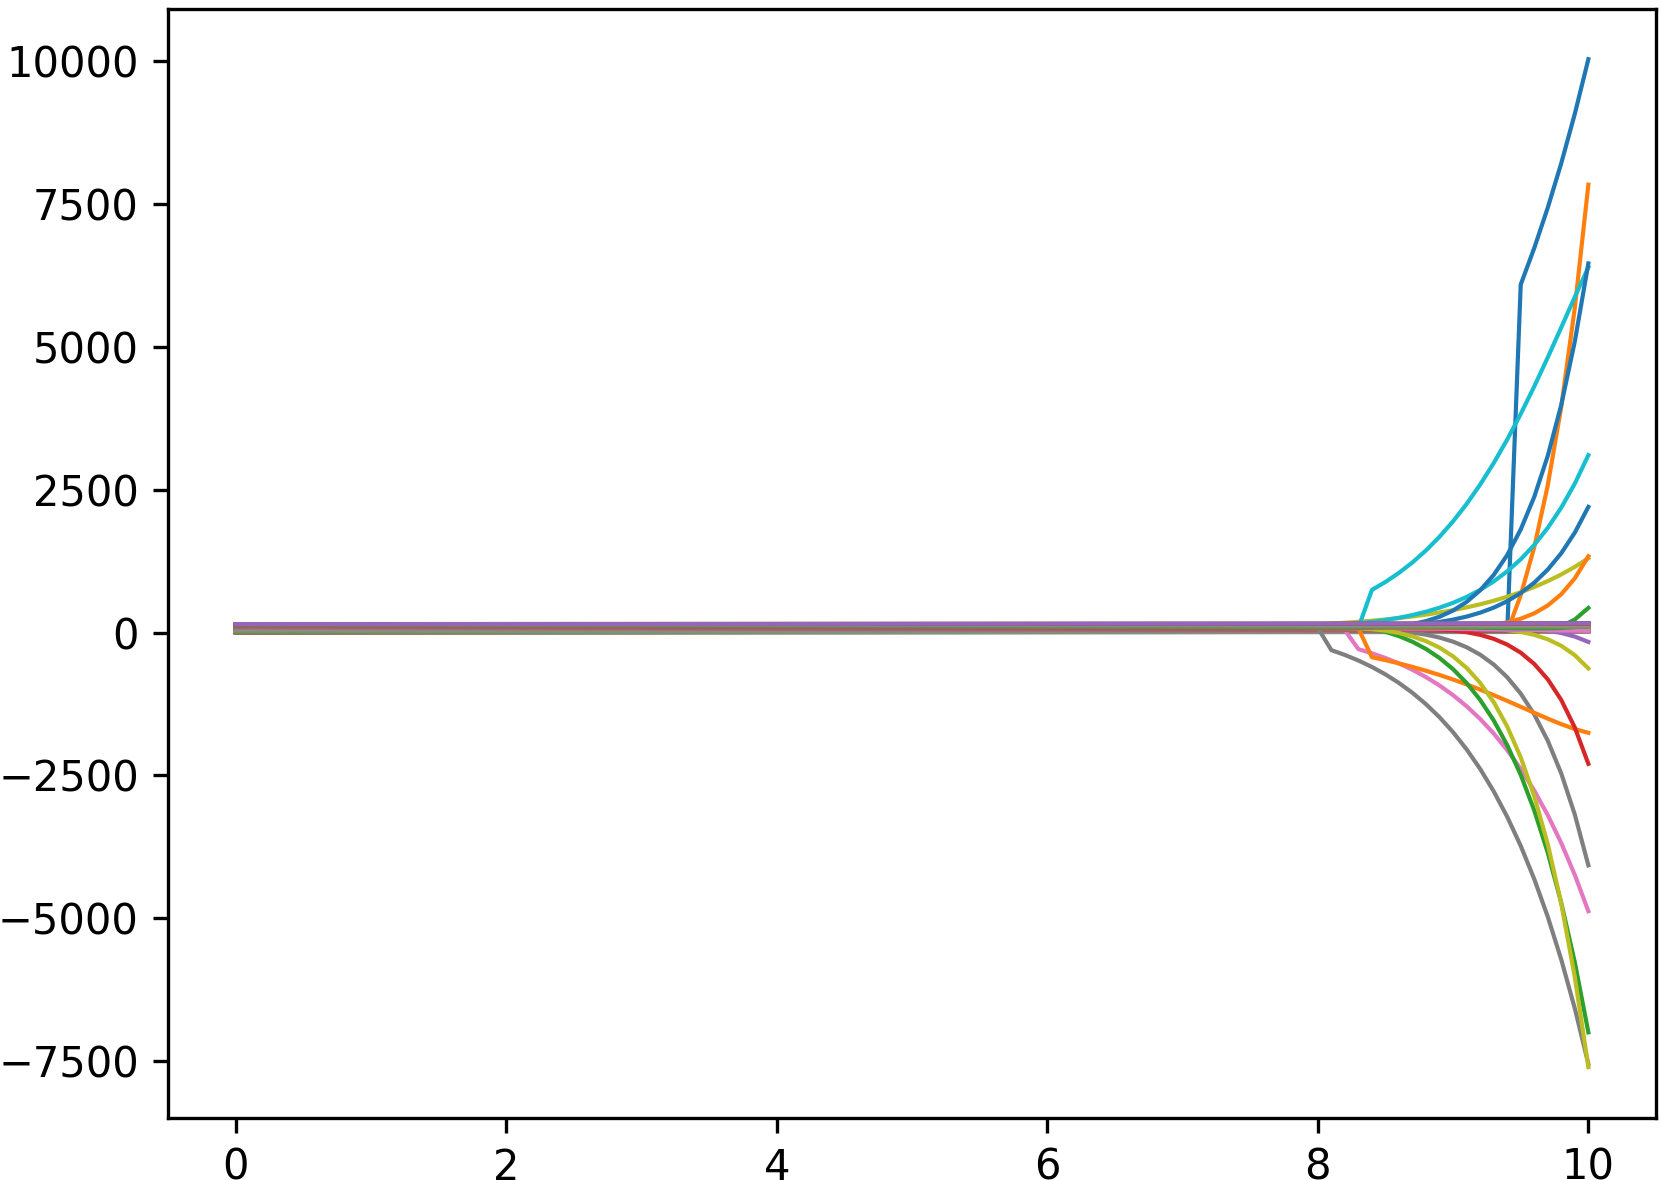
\includegraphics[width=0.6\textwidth]{failing_integration_rk4.png}
	\caption{Неуспешно интегриране на \textbf{ММ2} с RK4 при стъпка по времето $h = 10^{-5}$.}
	\label{fig:RK4_failing}
\end{figure}

\paragraph{RK45 (DOPRI5)} Една от класическите имплементации и най-популярна такава в различни софтуерни пакети на методи с адаптивен избор на стъпката е Dormand-Prince Runge-Kutta 4(5) (DORPI5) \cite{Dormand1980}. Той има известни предимства пред класическия вариант на Runge-Kutta-Fehlberg (RKF4(5)) \cite{Fehlberg1970} за твърди системи ОДУ, тъй като при RKF4(5) методът от четвърти ред има по-широк регион на стабилност и новата стъпка се избира от формулата за грешката на метода от четвърти ред. Това за случаите, когато областта на стабилност е малка (твърди ОДУ) може да доведе до ,,прескачането`` ѝ от метода от пети ред с избора на новата стъпка. Имплементацията на DOPRI5 е по-сложна, но този проблем с избора на стъпката е преодолян чрез по-сложен контрол на грешката. Тук ще използваме имплементацията на DOPRI5 от \textit{SciPy} с $rtol=10^{-6}$ като толеранс за грешката от интегриране.
\begin{figure}[hbpt]
    \centering
    \caption{Интегриране с RK45 (DOPRI5) при различни толеранси за относителната грешка.}
        \subfloat[$rtol = 10^{-6}$]{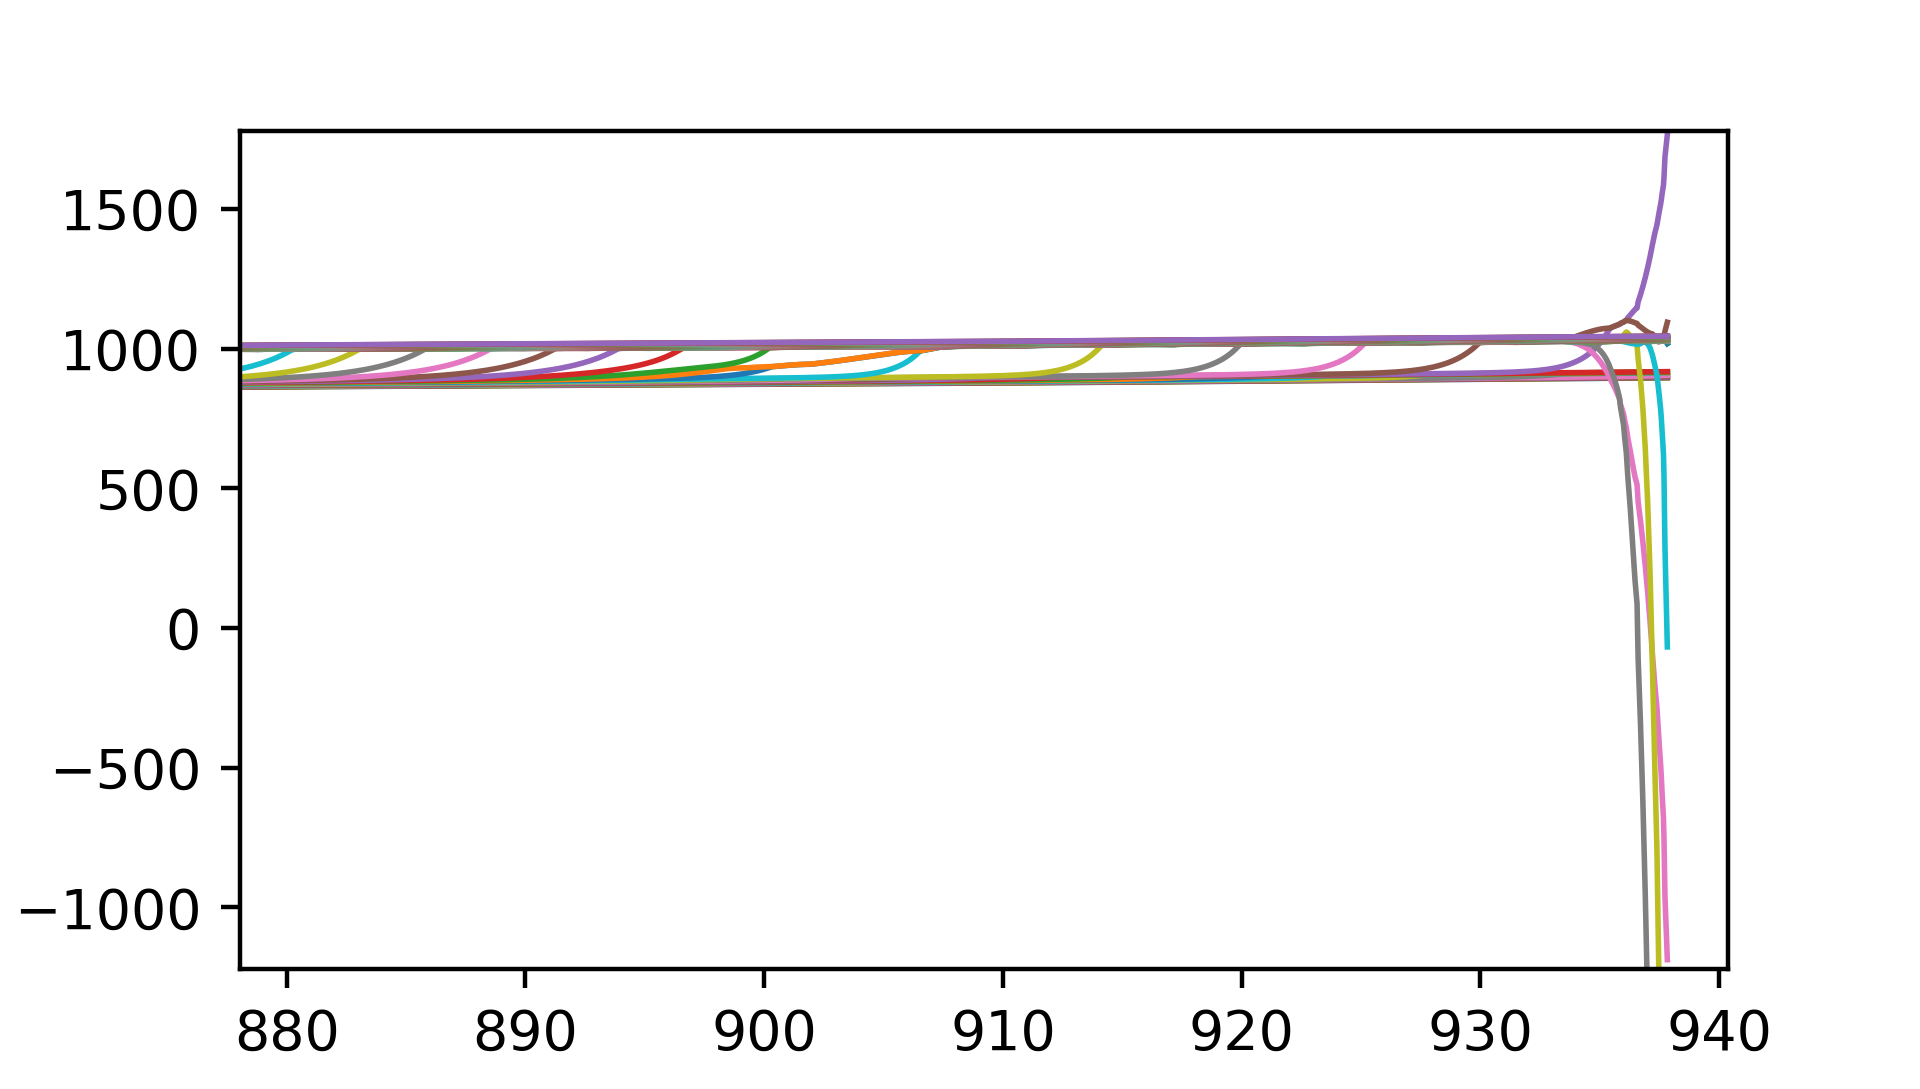
\includegraphics[width=0.4\textwidth]{almost_good_dopri5.png}}
        \subfloat[$rtol = 10^{-7}$]{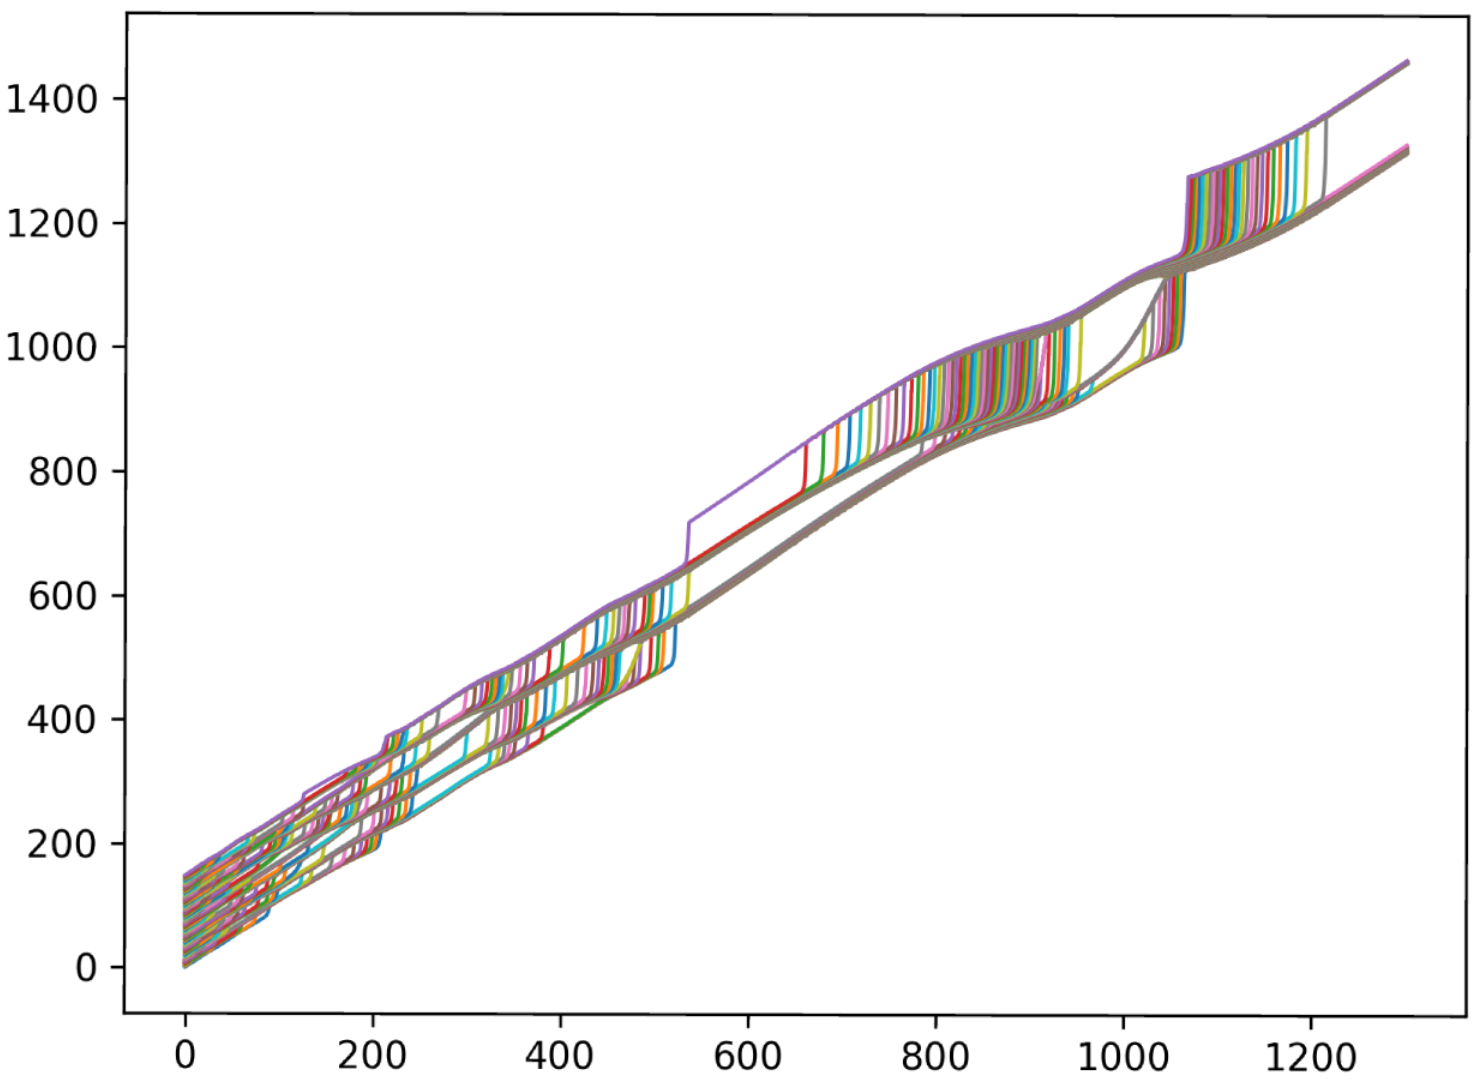
\includegraphics[width=0.3\textwidth]{good_dopri5.png}}
    \label{fig:dopri5_integration_results}
\end{figure}


\autoref{fig:dopri5_integration_results} ни показва, че при тези параметри можем да получим от DOPRI5 успешно интегриране, стига толерансът за грешката да е достатъчно малък $rtol  = 10^{-7}$. От \textbf{подфигура б)} дори можем да видим формираните групи в \textbf{MM2}.

Въпреки че за тези параметри на модела, DOPRI5 успява да интегриране система ОДУ, при по-голяма пертурбация на началната повърхност ($ > 20\%$), трябва да намалим $rtol = 10^{-9}$. Тези стойности стават от порядъка на машинната грешка за числата с плаваща запетая с единична точност. От друга страна, времето за получаване на решение става значително по-голямо. Това дава и причина да тестваме и други методи за решаване на тези системи ОДУ.

\paragraph{RK23} Е също метод с адаптивен избор на стъпката, който има по-нисък ред на точност от DOPRI5. Идеологията е същата, като RKF4(5), както и проблемите му. Удобното в случая е, че имплементацията е значително по-проста \cite{RK23GH}, както и броят на пътите, в които се изчислява дясната страна на ОДУ (по 3 пъти за всяка стъпка срещу 6 при DOPRI5). По-малкото пресмятания на дясната страна водят до потенциално по-добро поведение при твърди системи, заради намаления брой операции за една стъпка. \autoref{fig:rk23_integration_results} демонстрира именно това - за да е стабилно интегрирането е достатъчно толеранса в относителната грешка да е $rtol = 10^{-2}$. Проблемът на този метод е, че заради по-ниският ред на точност (трети), ако искаме да получаваме по-точни резултати за траекториите, той става значително по-бавен (броят на стъпките, които прави става много по-голям). По тази причина той също няма да е основният за целите на изследването, но е удобен за ,,бързи сравнения`` при различни модификации на ОДУ.
\begin{figure}[hbpt]
    \centering
    \caption{Интегриране с RK23 при различни толеранси за относителната грешка.}
        \subfloat[$rtol = 10^{-1}$]{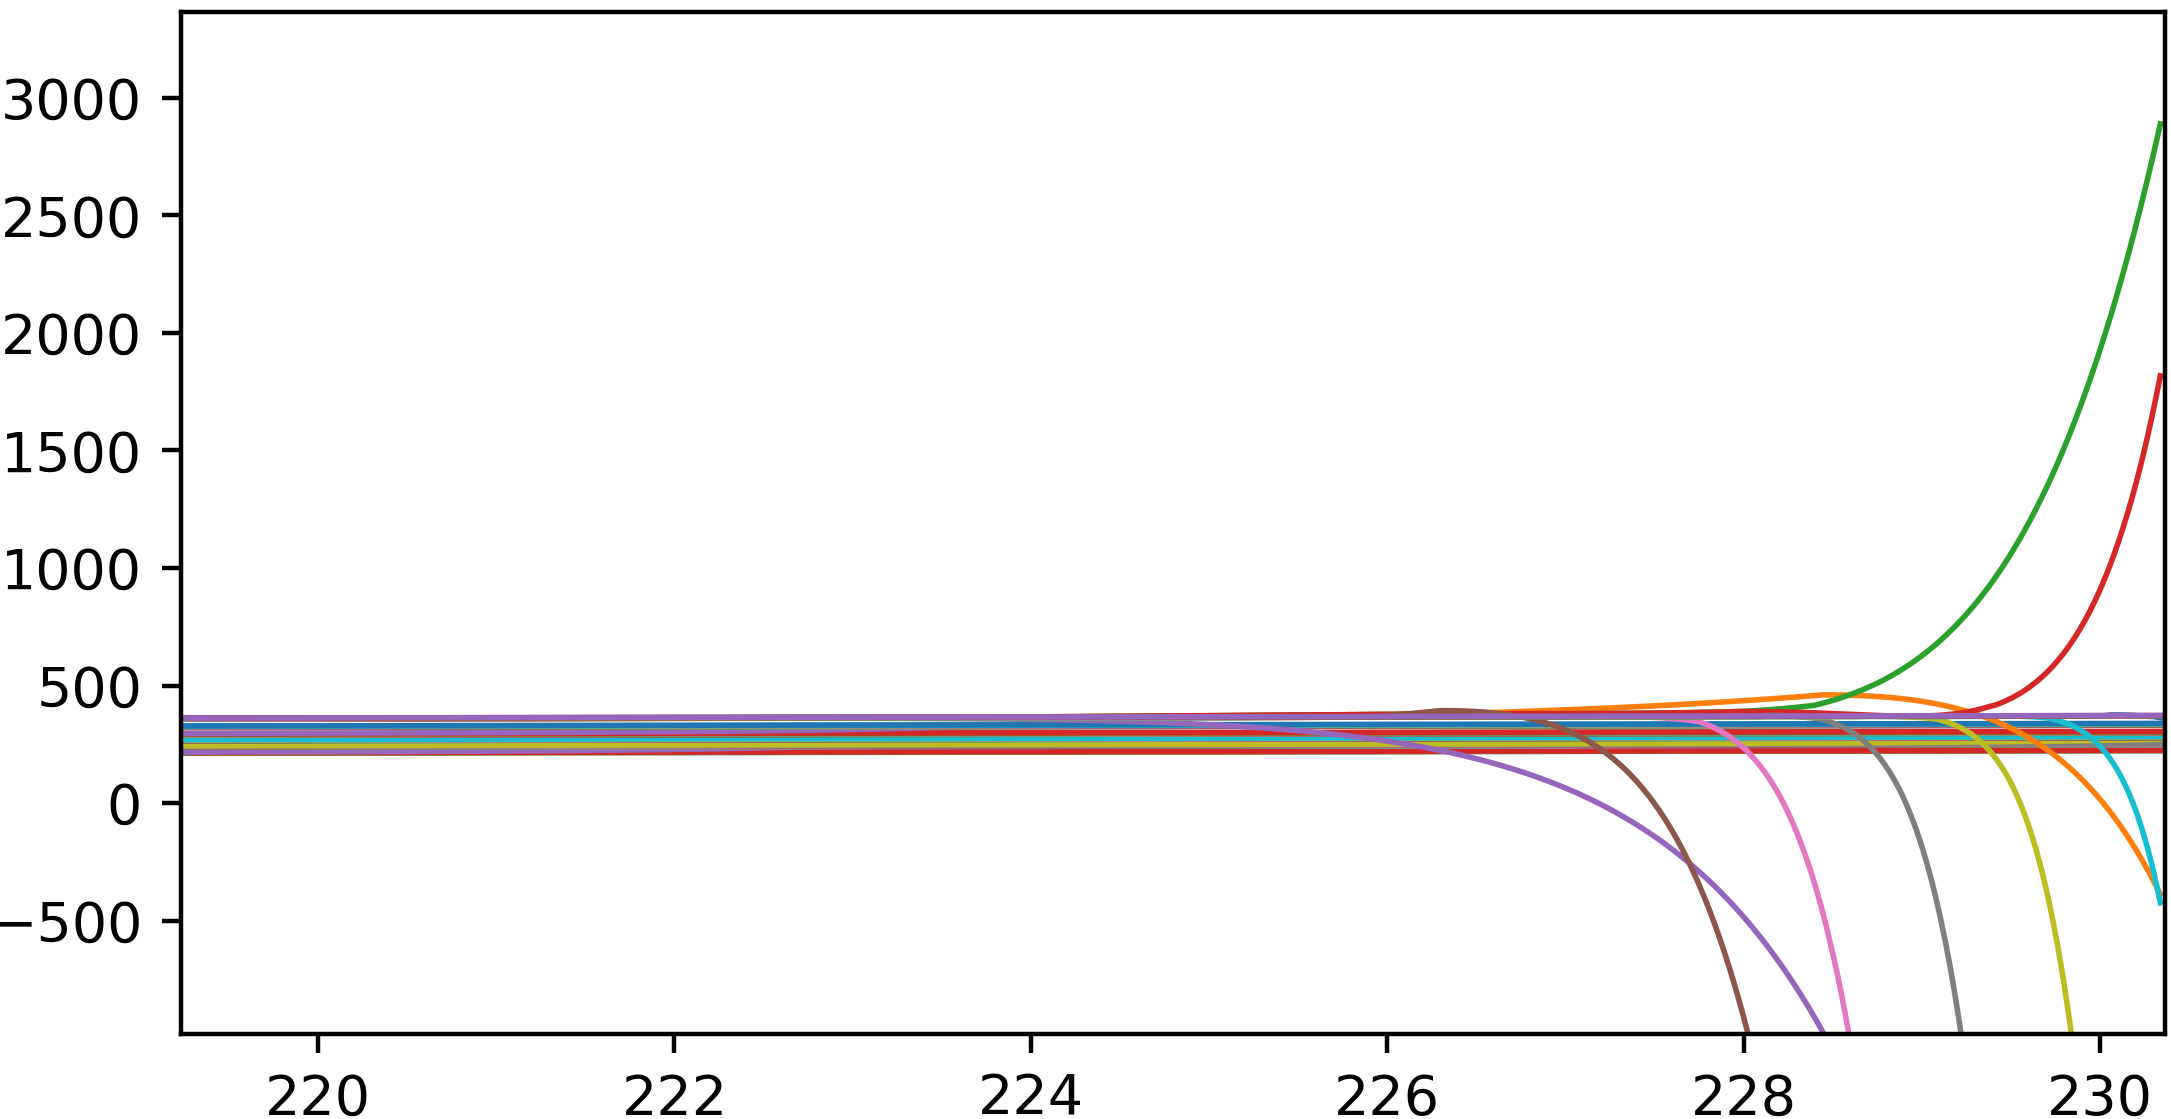
\includegraphics[width=0.42\textwidth]{bad_rk23.png}}
        \subfloat[$rtol = 10^{-2}$]{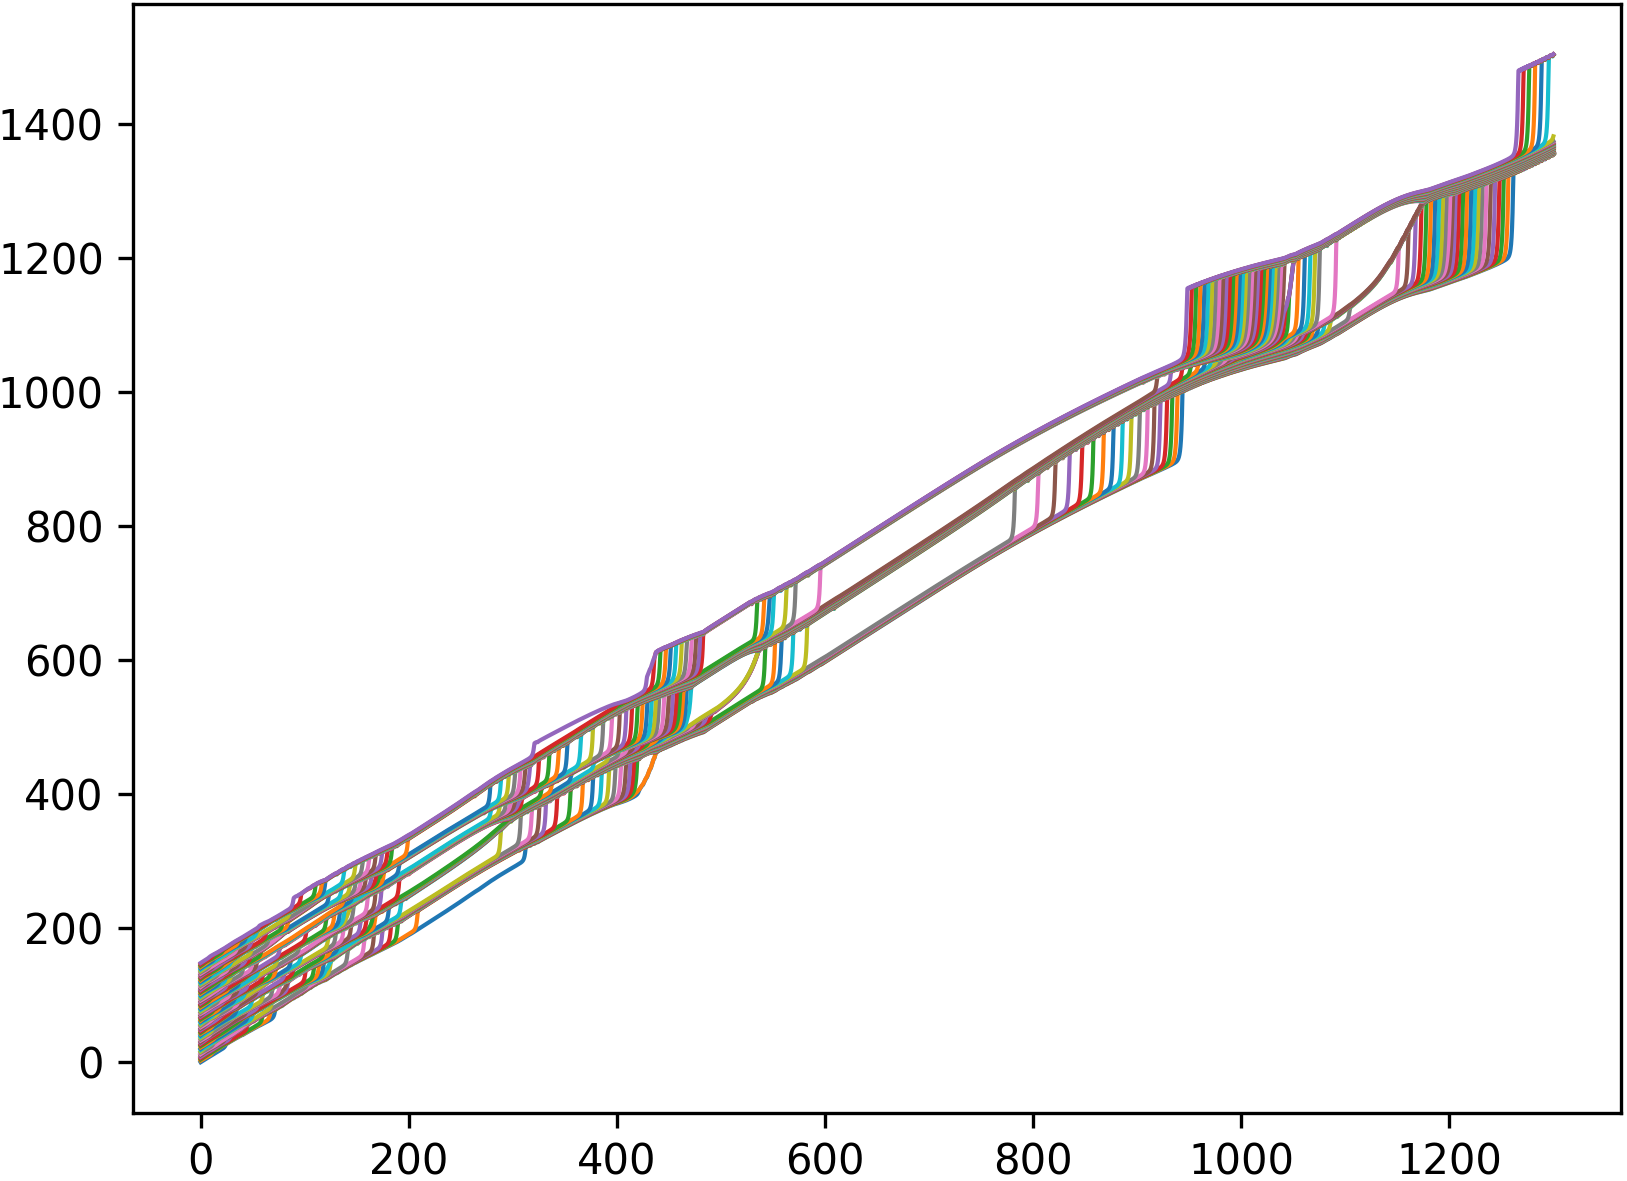
\includegraphics[width=0.3\textwidth]{good_rk23.png}}
    \label{fig:rk23_integration_results}
\end{figure}

\paragraph{LSODA/VODE} Са имплементации на \textit{variable-step-size-variable-order} (VSVO) методи на Адамс-Мултон (неявни методи на Адамс) за интегриране именно на твърди системи ОДУ \cite{Shampine2002}. Те са част от пакета за \textit{Fortran} ODEPACK \cite{odepack1992}, но имат програмни интерфейси за \textit{Python} в \textit{SciPy}, като последните предлагат и настройки по подразбиране за повечето от параметрите на съответния интегратор. \textit{LSODA} е по-комплексна имплементация от двата с автоматична смяна между методи \textit{stiff} и \textit{non-stiff} чрез член отчитащ ,,втвърдяването`` на системата, затова и ще предпочетем него. Резултатите наподобяват \autoref{fig:dopri5_integration_results} и \autoref{fig:rk23_integration_results}, като тук за $rtol < 10^{-7}$ интегрирането е успешно. Тук особеното е, че поради автоматичната смяна на метода и и адаптивната стъпка, интегрирането на системата отнема около 10 пъти по-малко време от DOPRI5. 

\paragraph{DE<XY>R} Са семейство методи за интегриране на твърди и не-твърди ОДУ публикувани от МГУ \cite{DEXYRD}. DE13R е вариант на RK4(5) с различен контролен член от RKF и DOPRI5, като резултатите от тестовете с него са аналогични на DOPRI5. DE21R е метод за твърди ОДУ с детектиране на ,,втвърдяването`` на системата ОДУ и адаптиране на реда/стъпката по съответен начин. Тъй като кодът на тези методи е само за \textit{Fortran 77} и \textit{C} се налага по подобен начин като за десните страни на моделите да се генерира обвивка/програмен интерфейс за \textit{Python}. Резултатите за DE21R са аналогични от LSODA с $rtol = 10^{-7}$, като и скоростта на интегриране е съизмерима. Неудобното тук е, че всеки от параметрите на интегратора трябва да бъде ръчно зададен и качеството на резултата силно зависи от това.

\subsubsection{Траектории на моделите}
В изследването на числените методи върху \textbf{MM2}, беше показан очаквания вид на траекториите за модел базиран на \autoref{eq:non_dimenisonal_ode}. Локалният наклон на кривите ни дава скоростта на стъпалата в дадения момент, а при фиксиран момент от време $t$ ,,напречното сечение`` на траекториите ни дава разстоянието между стъпалата и съответно броя на формираните групи с броя стъпала във всяка от тях - състоянието на повърхността в дадения момент.

\paragraph{MM2} Числените методи от предния параграф изпитвахме върху \textbf{ММ2} без особен коментар за получените траектории. Ще го интегрираме за параметрите описани за предни параграф и ще разгледаме получената траектория на \autoref{fig:MM_trajectory}.
\begin{figure}[htbp]
	\centering
	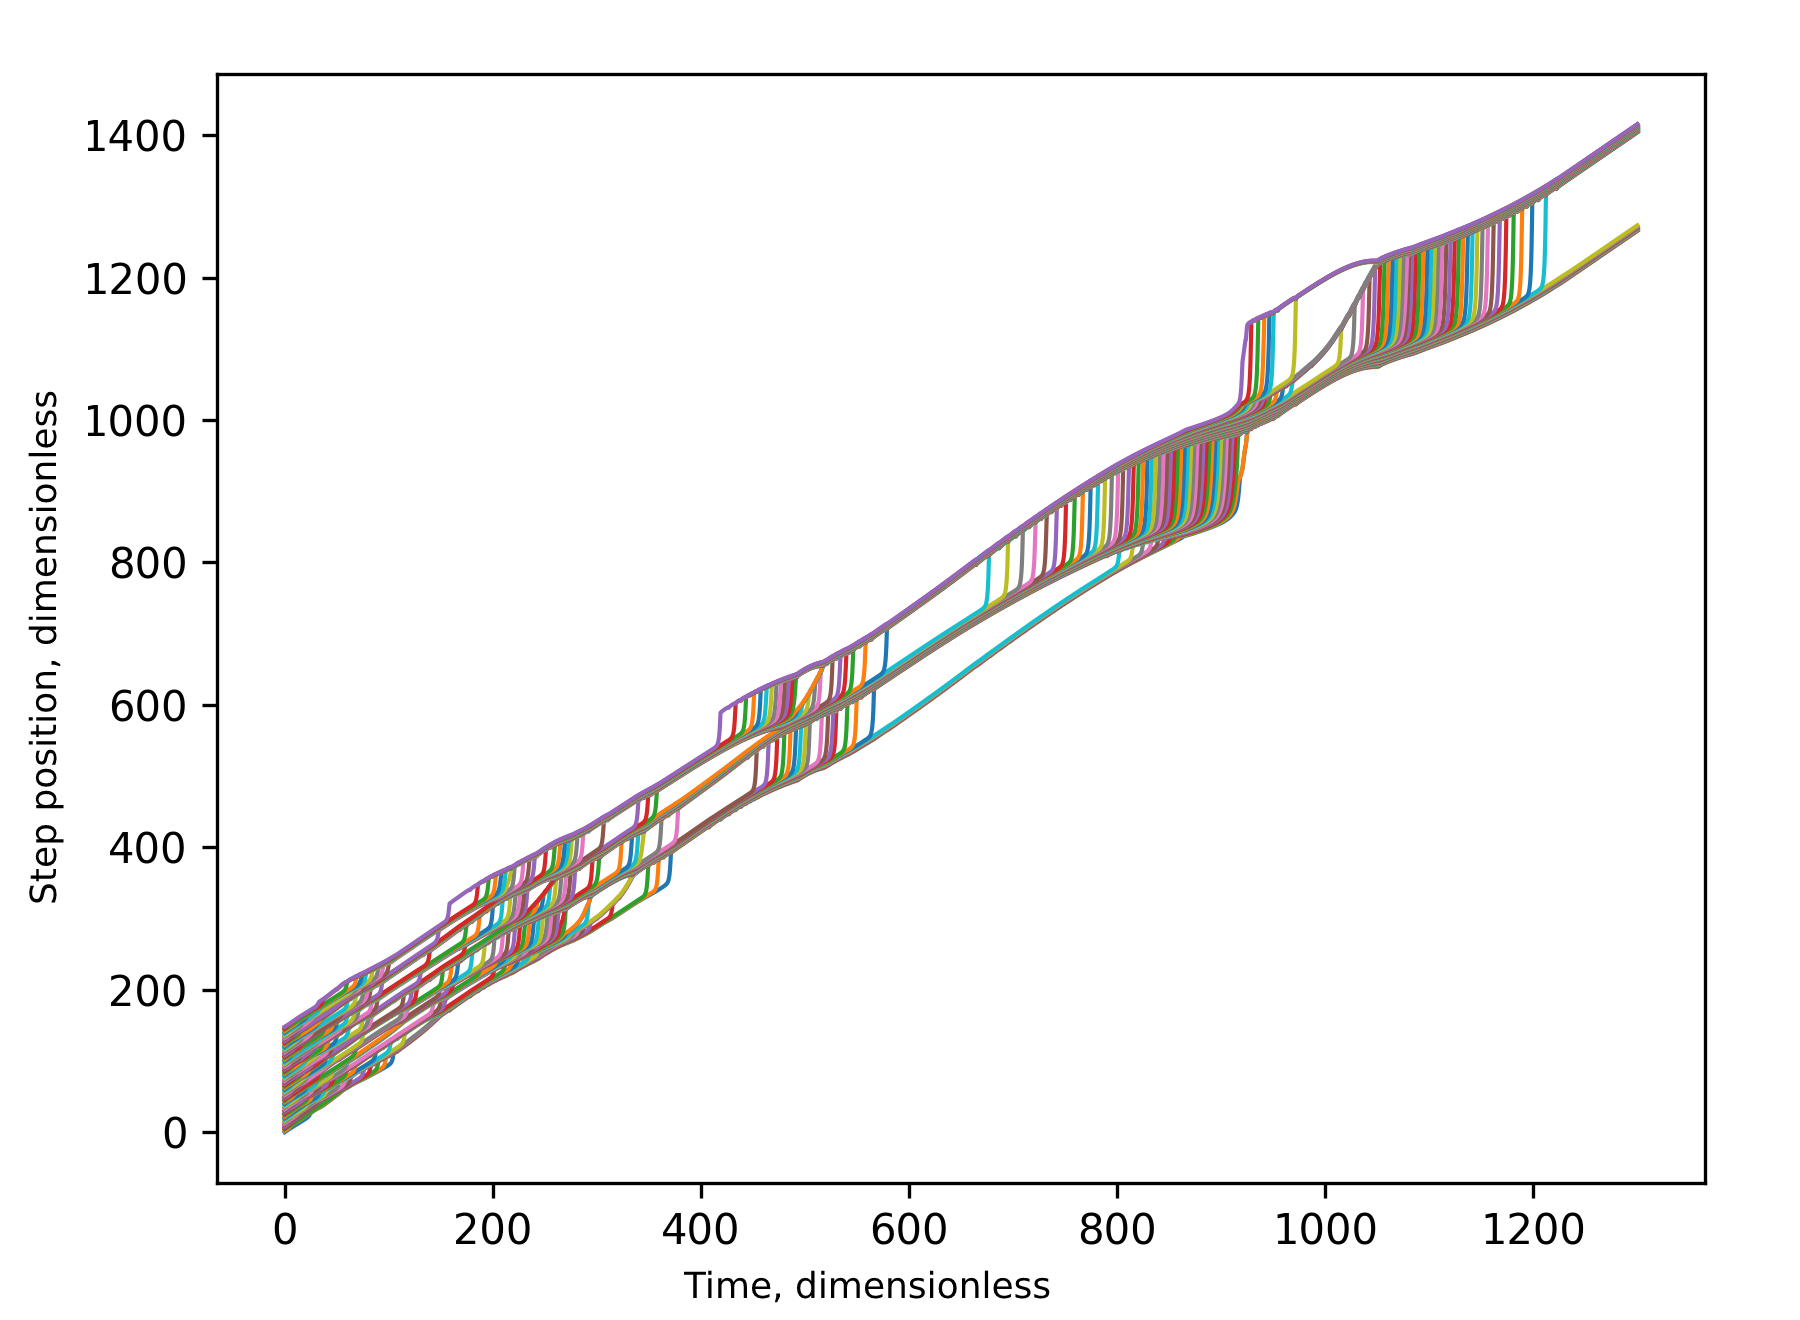
\includegraphics[width=0.7\textwidth]{g1smm.png}
	\caption{Траектория за \textbf{MM2} за 150 стъпала (изобразени 50)}
	\label{fig:MM_trajectory}
\end{figure}
При \textbf{MM2} започваме с пертурбирана начална вицинала, с развиването на процеса започват да се формират малки групи от по няколко стъпала, които в последствие коалесцират в по-големи чрез обмен на стъпала. Този процес доведен до края води до формирането на две големи групи, които поради периодичните гранични условия всъщност са една и съща голяма група. Можем да направим следните наблюдения на база представения числен експеримент и други аналогични: 
\begin{itemize}
    \item Моделът води успешно до групиране.
    \item Минималното разстояние между стъпалата с времето намалява, до формиране на една голяма група.
    \item В модела има т.нар. \textit{drift} - с времето групите се придвижват напред (наклонът на траекториите им е ненулев).
\end{itemize}
Можем чрез анализ на интензитета на пикселите на графиката с помощта на инструмента \textit{Fiji ImageJ} директно да получим визуално представяне на разстоянието между стъпалата в групите в определен момент. На \autoref{fig:MM_trajectory_profiles} от профилите в координати \textit{Gray Value vs. Distance (Pixels)} се виждат ясно формираните групи - при по-малкото време са 3, които в последствие са коалесцирали в две - по-големи.
\begin{figure}[hbpt]
    \centering
    \caption{Профил на траекториите от \autoref{fig:MM_trajectory} в различни моменти от безразмерното време t.}
        \subfloat[$t = 400$]{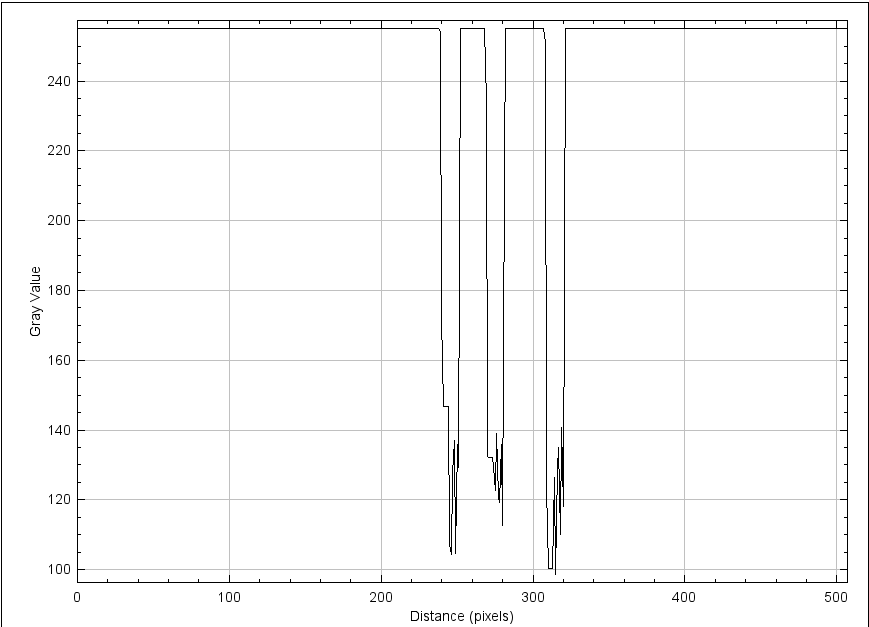
\includegraphics[width=0.38\textwidth]{g1smm_t400_profiles.png}}
        \subfloat[$t = 1200$]{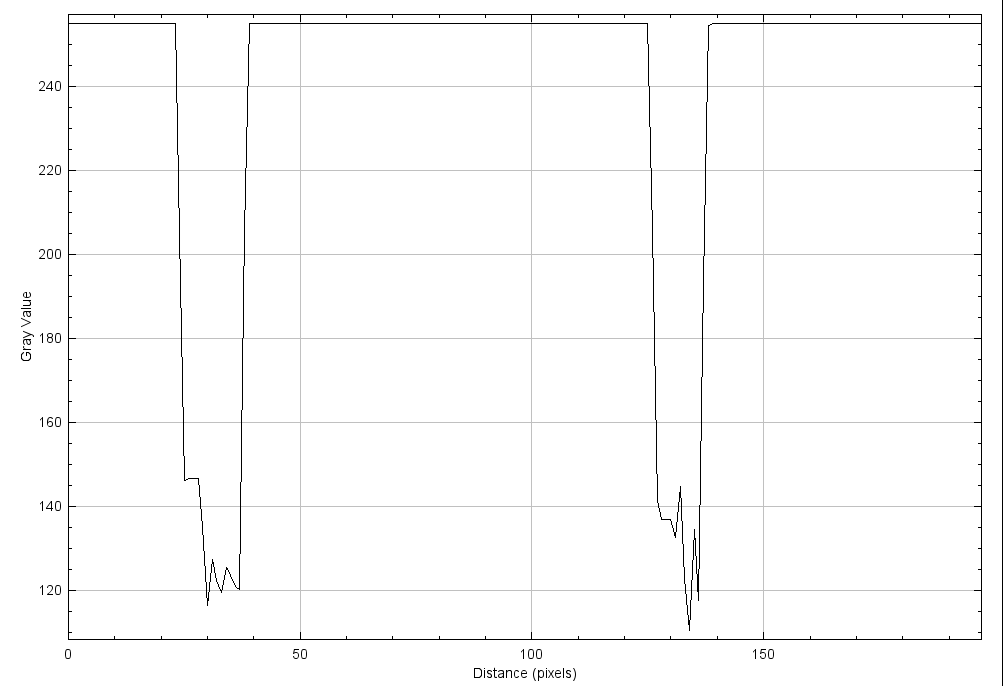
\includegraphics[width=0.4\textwidth]{g1smm_t1200_profiles.png}}
    \label{fig:MM_trajectory_profiles}
\end{figure}

\paragraph{LW2} Това e най-известният модел от \autoref{tabl:rhs_bunching_ode} и от разглеждания вид. Неговата имплементация отново е на \textit{Fortran}, като тук най-голям успех като бързодействие и устойчивост при промяна на параметрите имаме с RK23 интегратора. За експонентите в модела избираме стойностите от \textit{Liu \& Weeks} (1998) \cite{Liu1998} $p = 0$ и $n = 2$. Началното вицинално разстояние тук ще е преоразмереното $L_0$ спрямо анализа на размерностите, който беше направен в предните параграфи.
\begin{figure}[htbp]
	\centering
	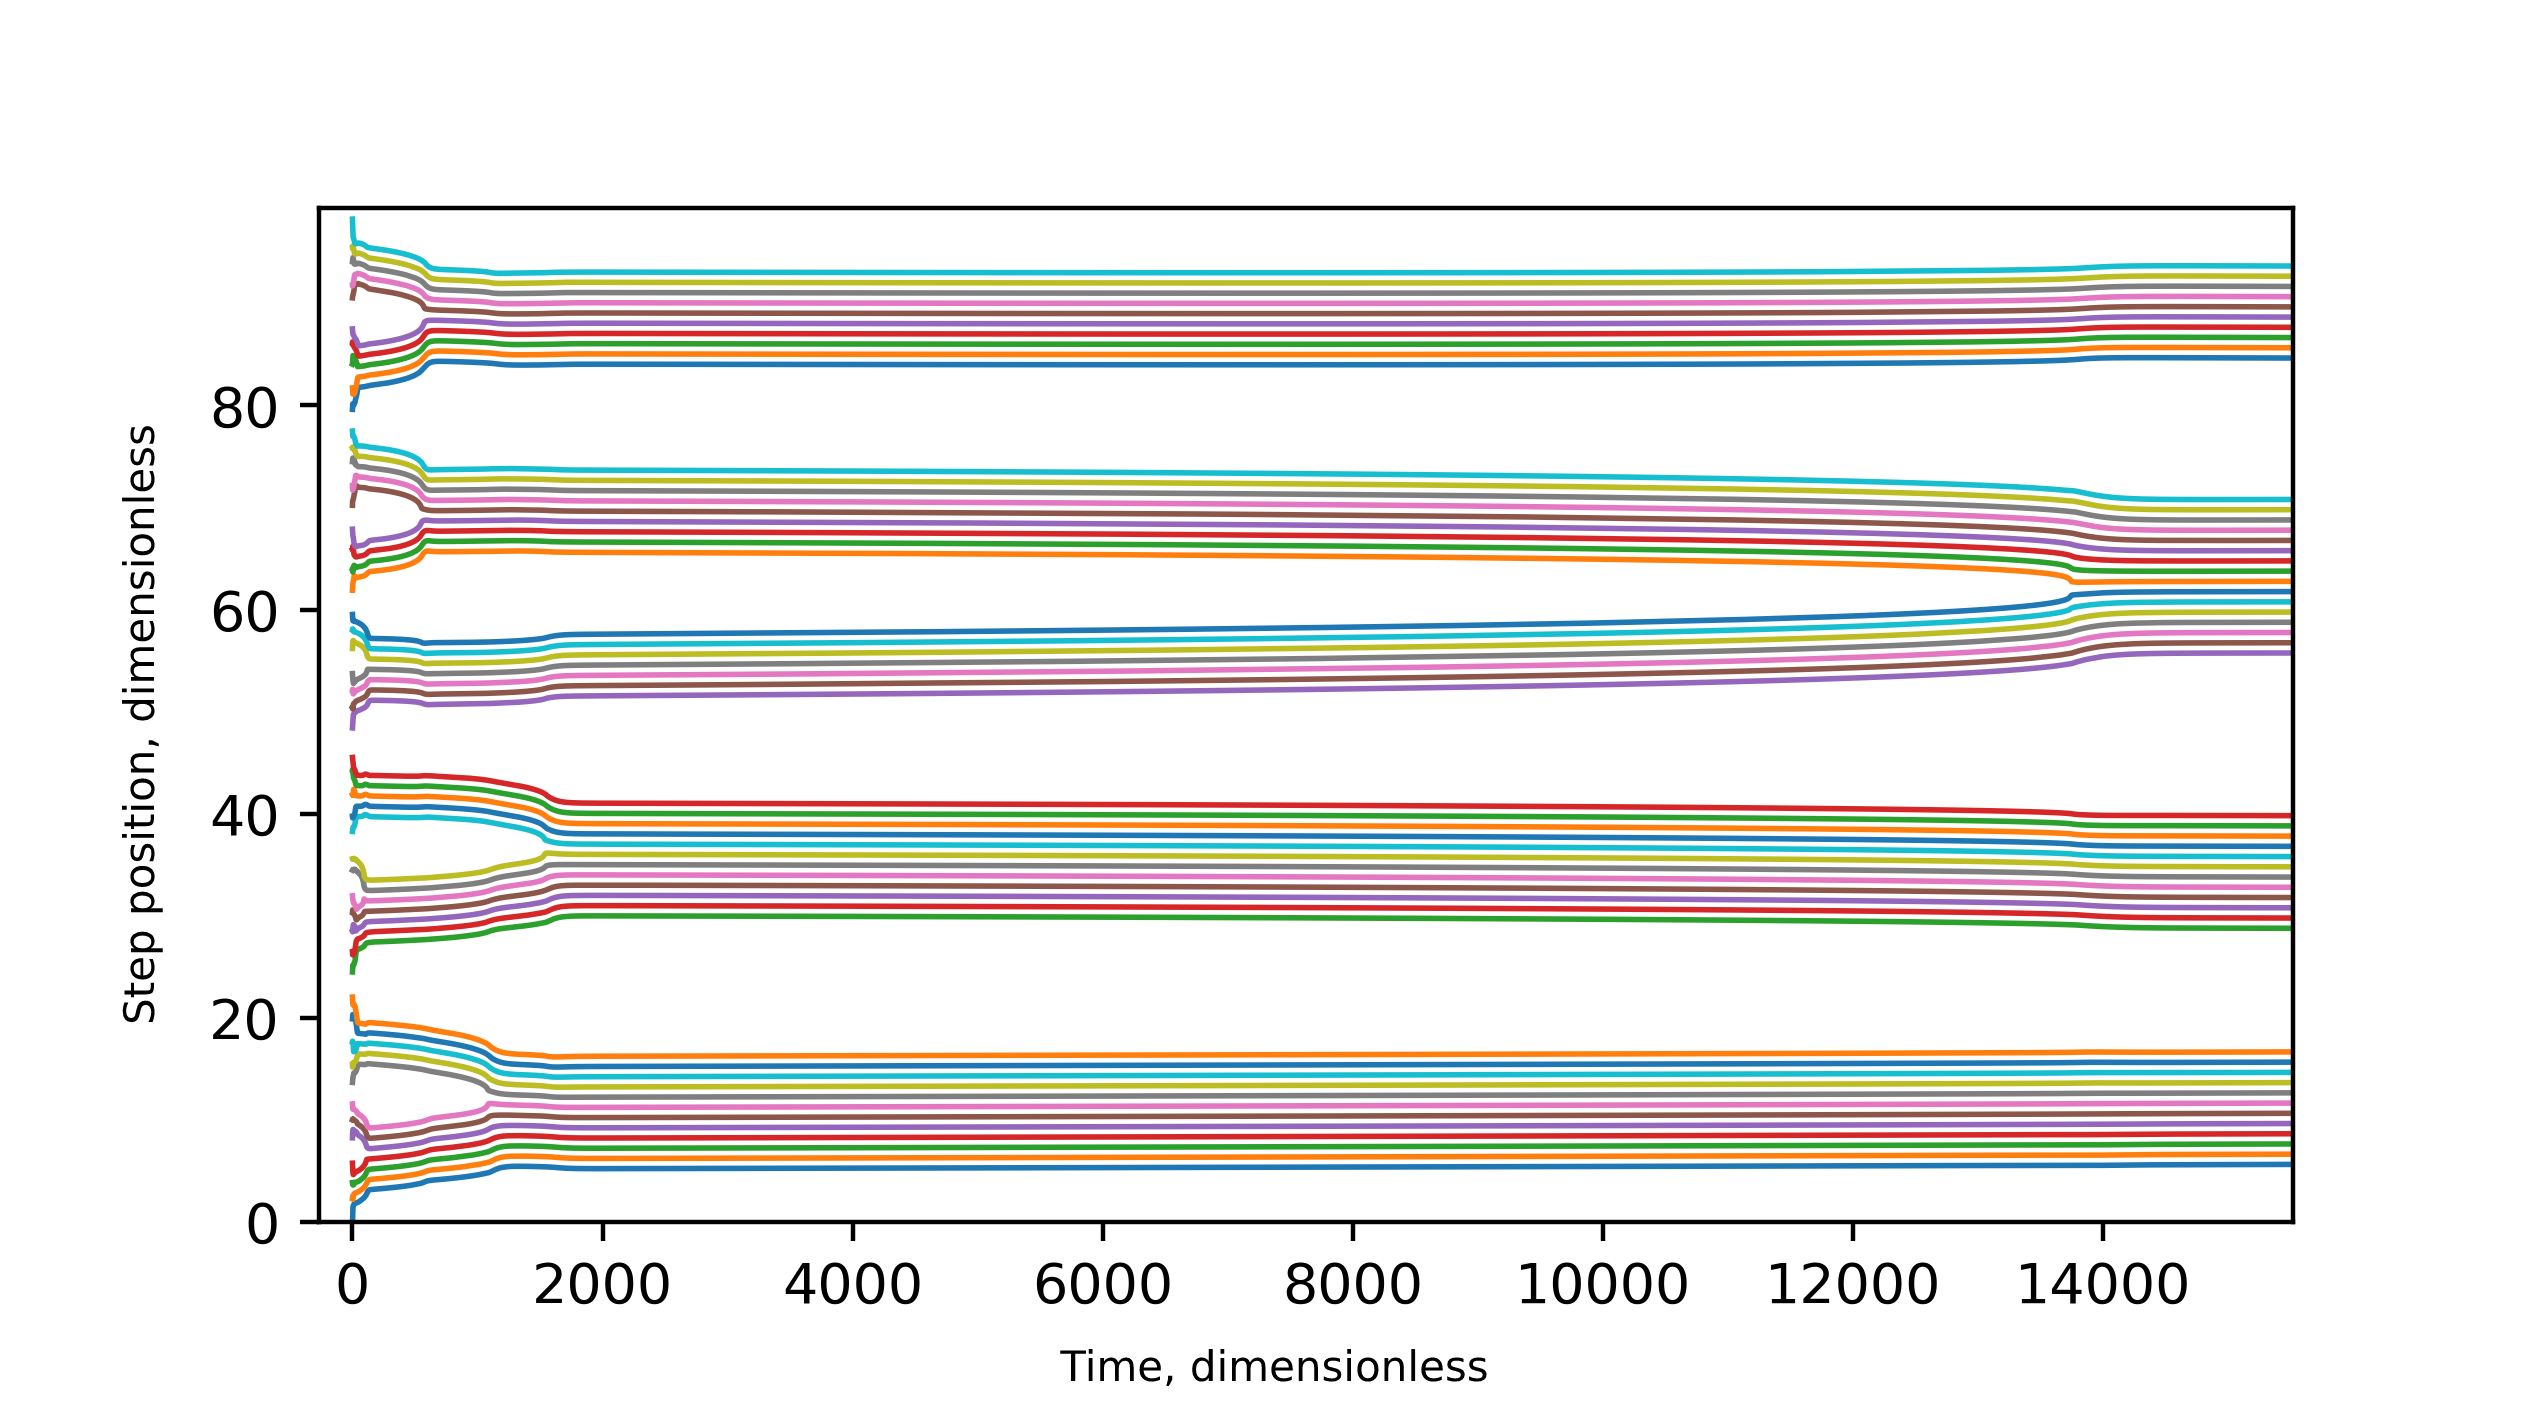
\includegraphics[width=0.80\textwidth]{lw_trajectory.png}
	\caption{Траектория за \textbf{LW2} за 150 стъпала (изобразени 50)}
	\label{fig:LW_trajectory}
\end{figure}
Наблюденията от числените експерименти тук и \autoref{fig:LW_trajectory} са следните: 
\begin{itemize}
    \item В \textbf{LW2} има групиране.
    \item Минималното разстояние в групите остава \textit{постоянно}, единствено броят на стъпалата в групите нараства (\textit{несвиваеми групи}).
    \item В модела \textit{няма} drift - наклонът на траекториите е ненулев само при сливане на две съседни групи, в останалото време те са статични.
    \item Времевата скала на този модел е \textit{значително} по-голяма от тази на \textbf{MM2} за съответните параметри.
\end{itemize}
\autoref{fig:LW_trajectory_profiles} представя отново анализ на профилите на траекториите за две различни безразмерни времена. Добре се вижда, че разстоянието в пиксели между стъпалата (пиковете) е относително постоянно за две различни времена ($t = 2000$ и $t = 14000$). С времето отново малките групи коалесцират в по-големи такива, което се вижда добре на профилите. При достатъчно дълго време на интегриране дори тези 4 (3 през периодичните г.у.) ще станат една, подобно на \textbf{MM2}. Тъй като тук времевата скала е значително по-голяма, това отнема значително изчислително време и прави трудно визуализирането на траекториите на една статична графика.
\begin{figure}[hbpt]
    \centering
    \caption{Профил на траекториите от \autoref{fig:LW_trajectory} в различни моменти от безразмерното време t.}
        \subfloat[$t = 2000$]{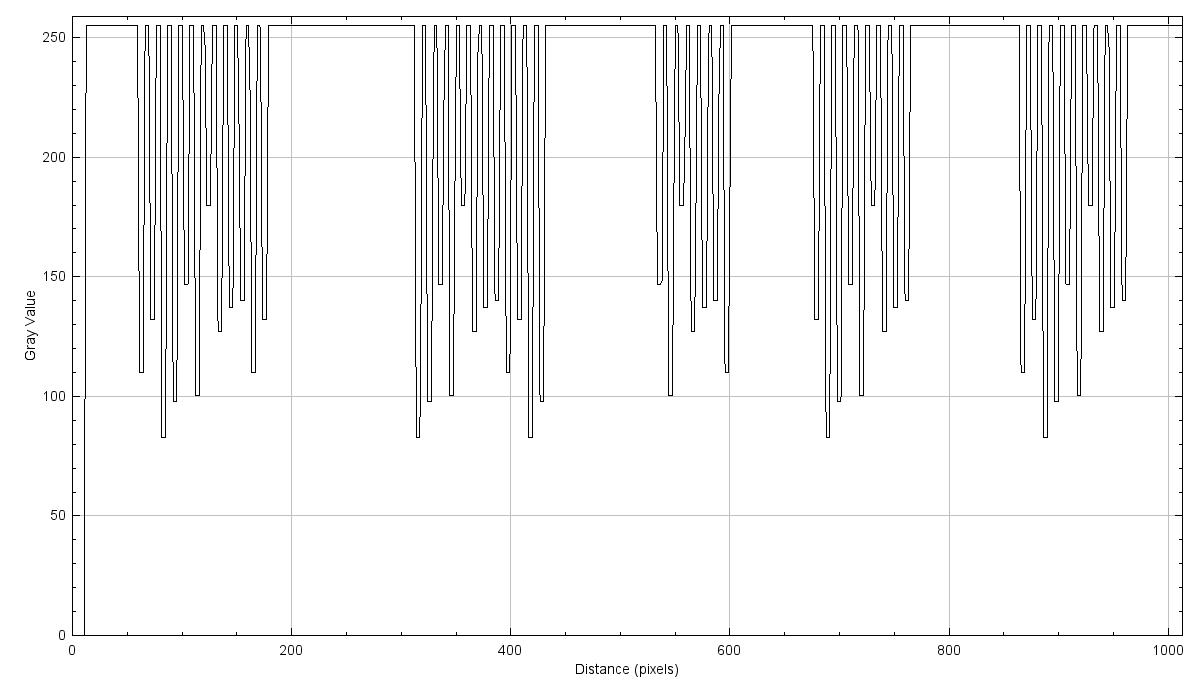
\includegraphics[width=0.37\textwidth]{lw_profile_t2000.png}}
        \subfloat[$t = 14000$]{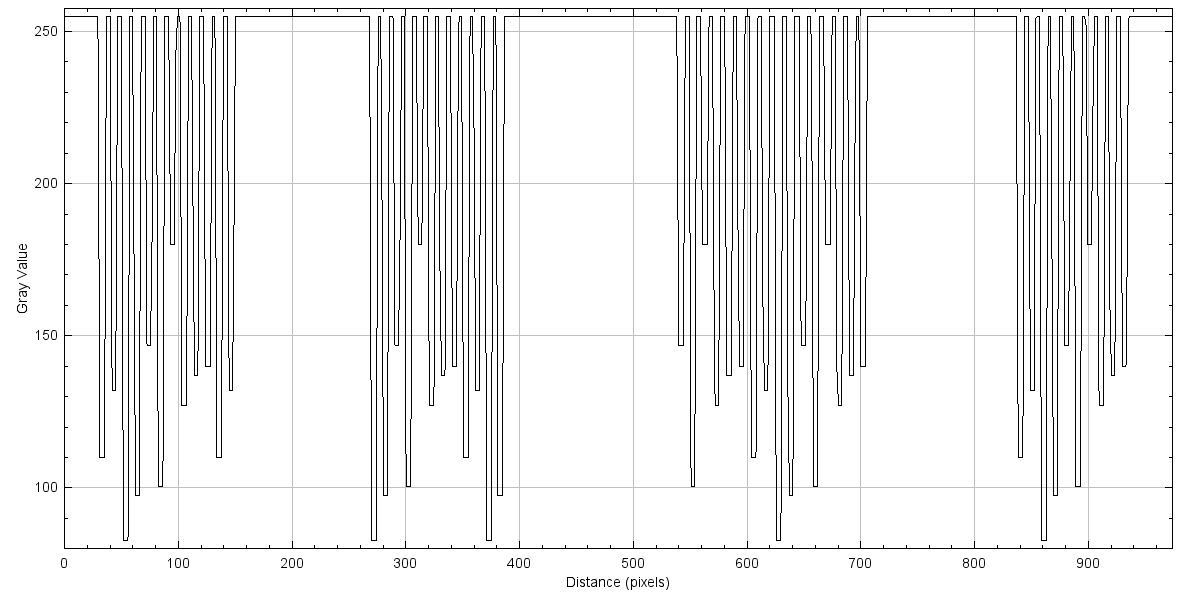
\includegraphics[width=0.41\textwidth]{lw_profile_t14000.png}}
    \label{fig:LW_trajectory_profiles}
\end{figure}

\paragraph{TE} Това е най-старият (исторически) от моделите и с най-сложен вид на дясната страна. Тук особено е, че участва $i+2$-тераса - взаимодействията са по-далечни и изискват по-внимателно третиране на периодичните г.у. Отново интегрираме за $p = 0$, $n = 2$ като ,,канонични`` от \textit{Tersoff} (1995) \cite{Tersoff1995}, като пример за получена траектория е даден на \autoref{fig:TE_trajectory}.
\begin{figure}[htbp]
	\centering
	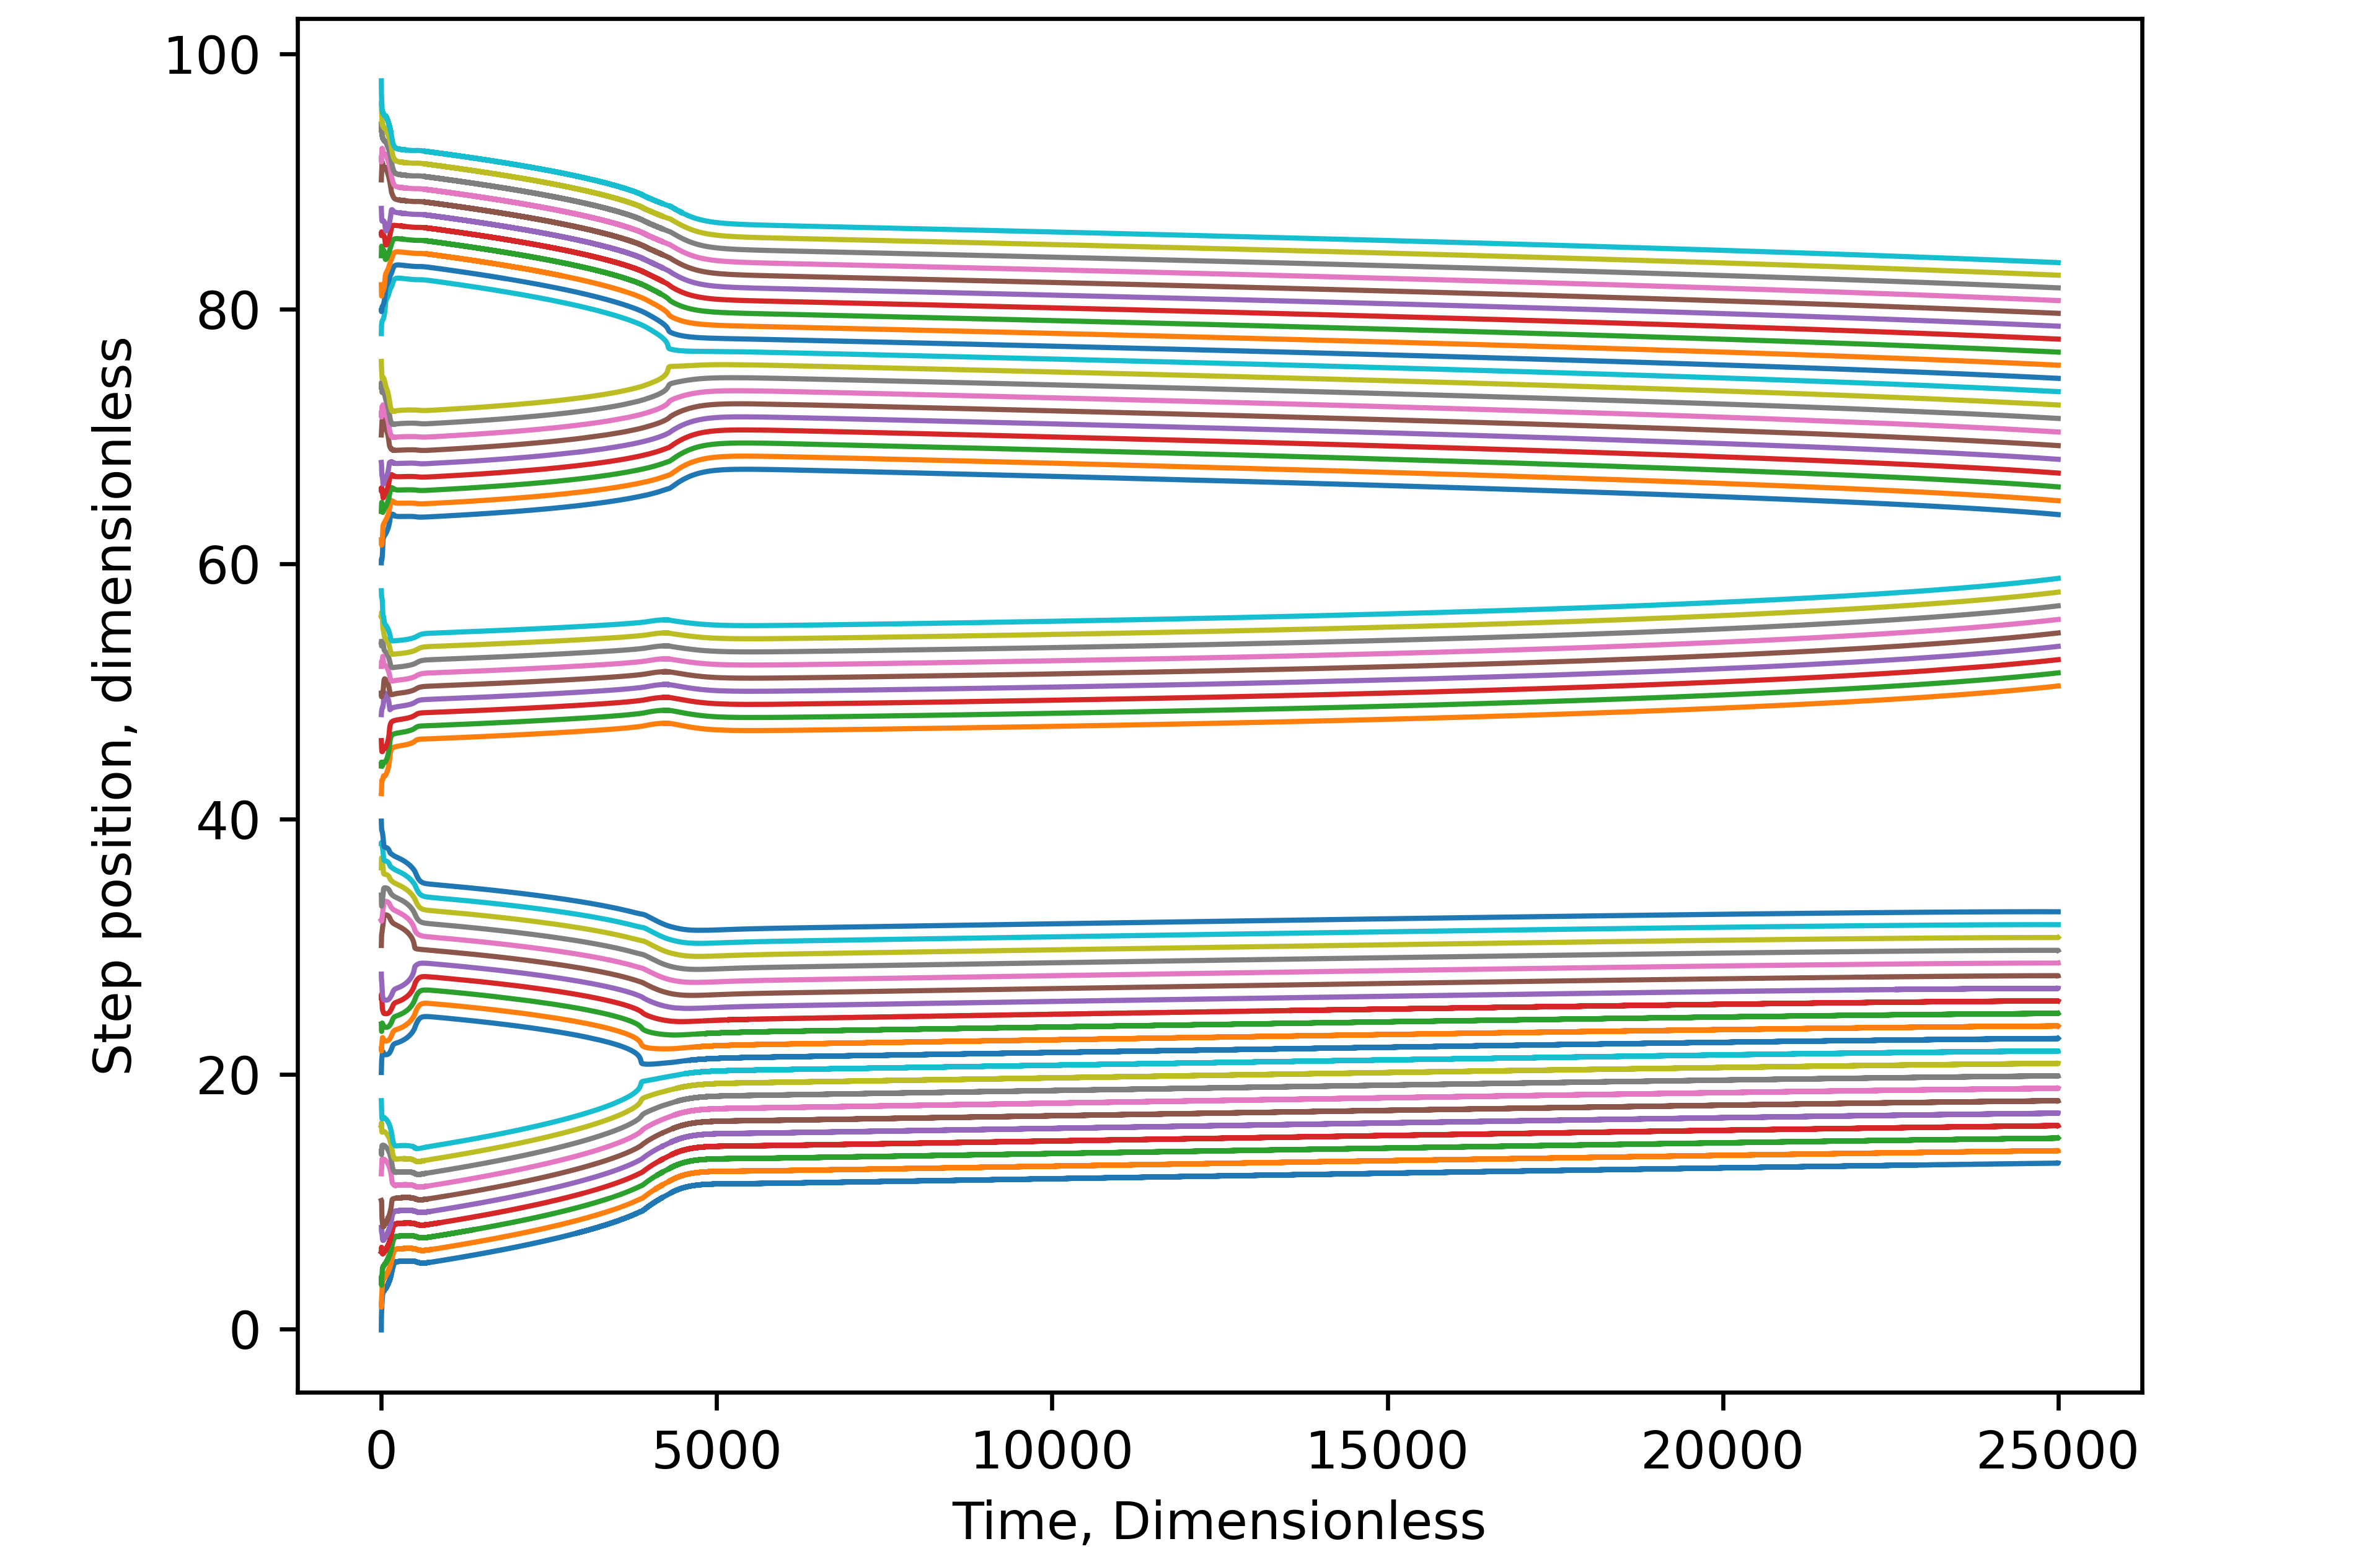
\includegraphics[width=0.80\textwidth]{te_trajectory.png}
	\caption{Траектория за \textbf{TE} за 150 стъпала (изобразени 50)}
	\label{fig:TE_trajectory}
\end{figure}
Резултатите (визуално и като времева скала на процеса) са много подобни на тези за \textbf{LW2}. Особеното тук e, че в оригиналния труд на \textit{Tersoff} се сумира до ,,безкрайност``, т.е. всички тераси имат принос за $i$-тото стъпало. Това означава, че трябва да имаме много големи системи и да се изследва асимптотичното поведение на системата при нарастване на броя съседи в модела.
\begin{figure}[hbpt]
    \centering
    \caption{Профил на траекториите от \autoref{fig:TE_trajectory} в различни моменти от безразмерното време t.}
        \subfloat[$t = 5000$]{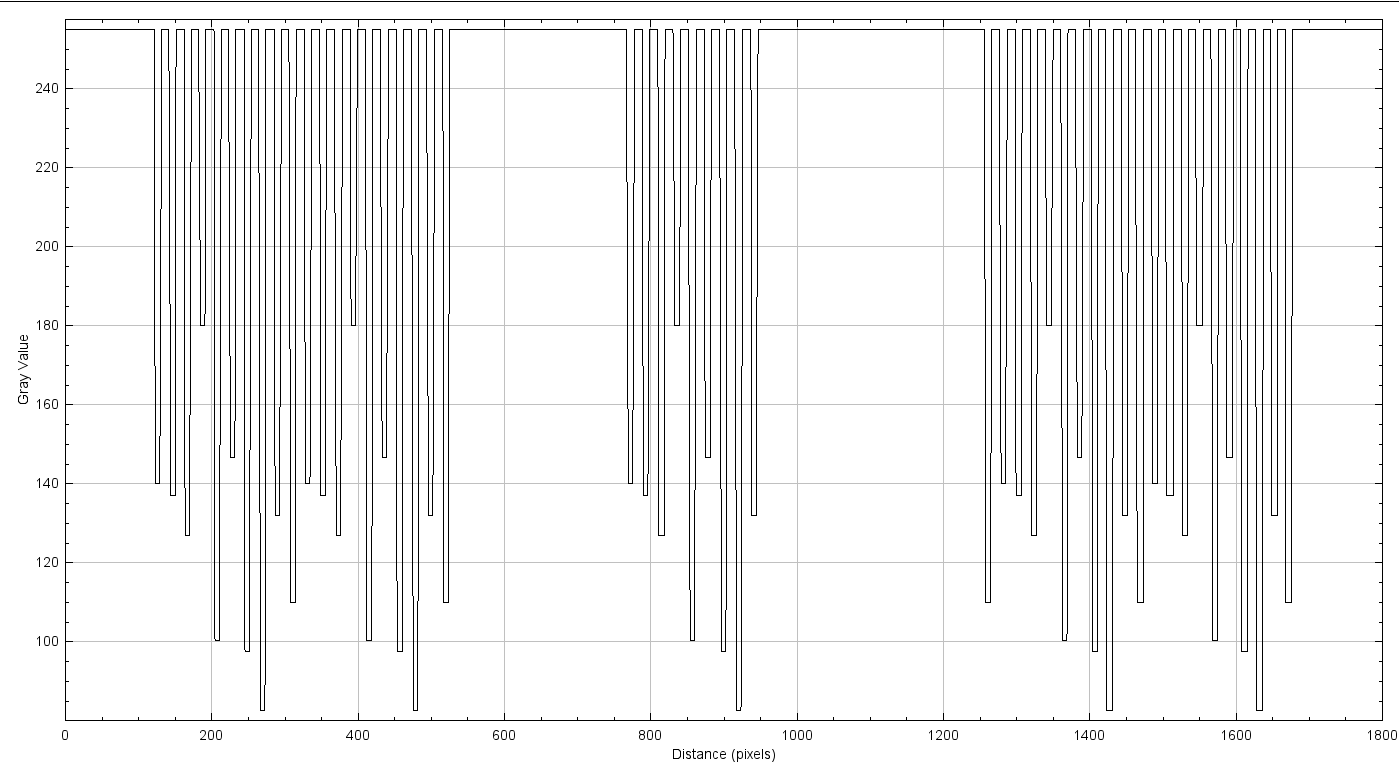
\includegraphics[width=0.4\textwidth]{te_t5000_profiles.png}}
        \subfloat[$t = 25000$]{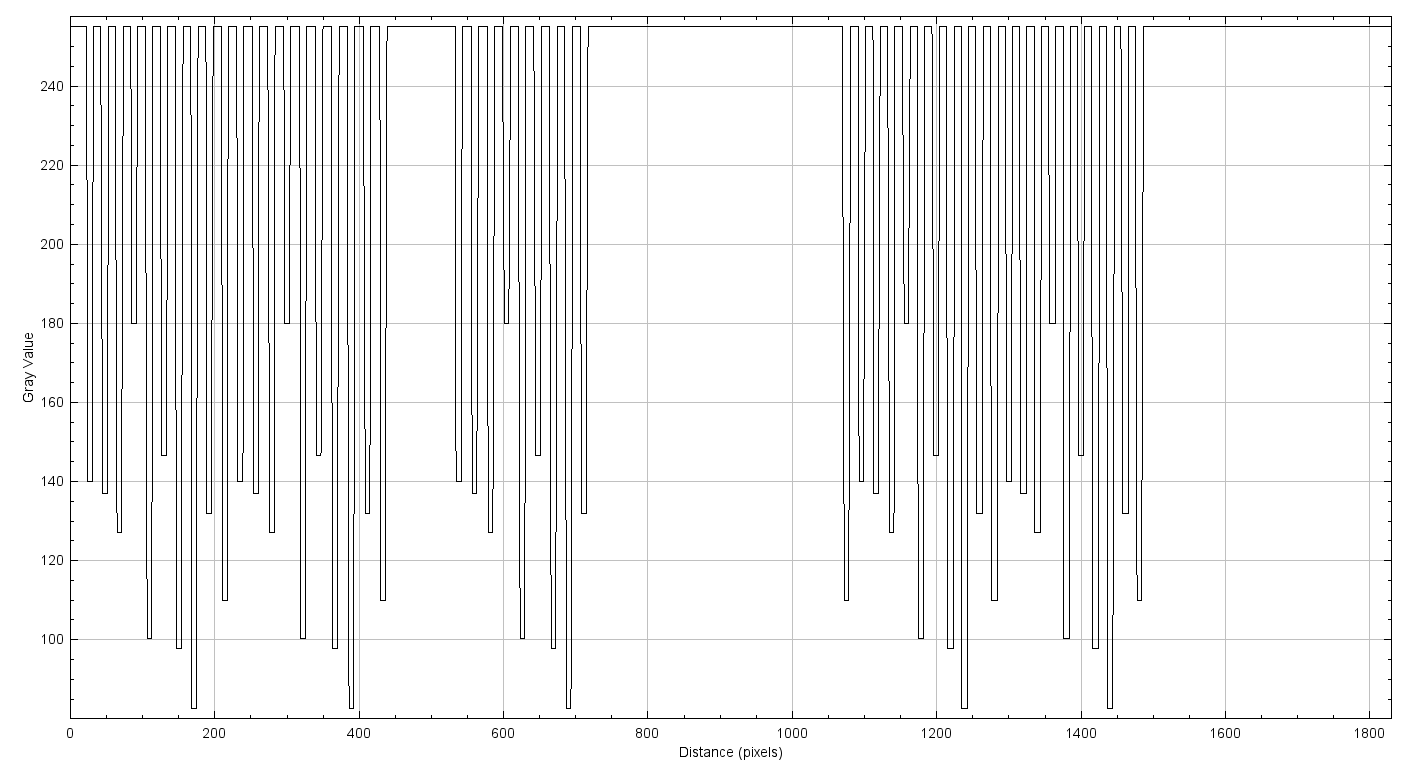
\includegraphics[width=0.4\textwidth]{te_t25000_profiles.png}}
    \label{fig:TE_trajectory_profiles}
\end{figure}
Групите на модела на \textbf{TE} отново са несвиваеми и нямат drift, като при избраното обезрамеряване минималното разстояние при формирани стабилни групи е $l_{min}/L_{0} = 1$. 

\autoref{fig:TE_trajectory_profiles} демонстрира предстоящото сливане на две големи групи при развитието на процеса, отново асимптотично в края на процеса ще има единствена голяма група, която се пропагира с времето устойчиво.

\subsubsection{Схеми за мониторинг и видове групиране}
Профилите получени с \textit{Fiji ImageJ} са удобна визуализация на развитието на повърхността, но не са количествена информация, с която можем да получим скейлинговите зависимости на характеристики като брой стъпала и минимално разстояние в групата по отношение на времето. Искаме да можем да изследваме числено автомоделната функция от \autoref{eq:dimensional_scaling}. По тази причина е необходима процедура, с която систематично да бъдат изследвани характеристиките на повърхността. \textit{Тончев (2012)} \cite{tonchev2010scaling} предлага две \textit{схеми за мониторинг}, които именно от резултантните на интегриране траектории изчисляват среден брой стъпала в групата, минимално разстояние в групата, средна ширина на терасата и т.н. 

За схемите на мониторинг централен параметър е \textit{bunch definition - bdef}. Това е разстоянието, под което смятаме, че две стъпала принадлежат на една група или обратното - на две различни групи и от правилния му избор зависи до голяма степен успеха на процедурите.

\paragraph{Monitoring Scheme I (MSI)} e процедура за ,,snapshot statistics`` \cite{TonchevArxiv2012} - работи върху моментното състояние на повърхността, без да взима предвид предишната ѝ еволюция. Това е подобно на анализ на профилите получени от \textit{Fiji ImageJ}. За целите на схемата, на всяка стъпка по времето от траекторията изчисляваме броя на групите в системата, средния брой стъпала в групата $N$ и съответните допълнителни величини - брой тераси и тяхната средна ширина, както и глобално най-малкото разстояние в групите $l_{min}^g$. Динамичният скейлинг на всяка от тези зависимости след това може да бъде изследван поотделно, като ги разгледаме $\log\mbox{--}\log$ координати.

\paragraph{Monitoring Scheme II (MSII)} е кумулативна статистика по размера на групите \cite{TonchevArxiv2012}. В този случай се проследява за даден размер група еволюцията на средната ширина на групата, минималното разстояние в групата $l_{min}$. На всяка стъпка от се използва MSI, за да се намерят съответните размери на групите и тогава на база резултатите от MSI и информацията за всички предишни стъпки от MSII се изчисляват съответните характеристики. Така могат да се разкрият по-фини скейлингови зависимости зависимости за процеса на групиране.

\textit{Станева и сътрудници (2012)} \cite{Staneva2012} дефинират два фундаментални типа групиране \textbf{B1} и \textbf{B2}. Те са основни за осмислянето на голямото разнообразие от модели на феномена, както и определяне на ,,съвместимостта`` на даден модел с конкретни експериментални данни:
\begin{itemize}
    \item \textbf{B1} типа групиране се характеризира с \textbf{постоянно} $l_{min}$ в групата и само \textbf{една} характеристична скала за дължина необходима за описание на процеса.
    \item \textbf{B2} се характеризира с \textbf{намаляващо} $l_{min}$ в групата и \textbf{две} характеристични скали за дължина необходими за описание на процеса.
\end{itemize}

Тъй като в \textbf{B1}-тип моделите $l_{min}$ остава постоянно, то за пълното изследване на скейлинговите зависимости при тях е достатъчно да използваме \textit{само} MSI. Изследваните в настоящия текст модели имат една скала за дължина ($\xi_0$) \cite{Staneva2010} и те са съответно \textbf{B1}-тип.

\subsubsection{Скейлингови зависимости на ОДУ моделите}
MSI е имплементирана, така че да работи директно със записаните след интегрирането траектории. За всеки от трите модела ще изследваме конкретно зависимостите $N \propto t^\beta$. 

\paragraph{LW2} За \textbf{LW2} е известно от литературата \cite{Liu1998} \cite{Krasteva2016}, че за фиксирано $n = 2$:
\begin{equation}
    \beta = \frac{1}{p+5}
    \label{eq:lw_scaling_beta}
\end{equation} 
Интегрираме траекториите за $p = 0, 1$ и съответно пресмятаме средният брой стъпала в групата $N$ във всеки един момент от времето. В логаритмични координати наклонът $a$ на линейната зависимост $\log(N) = a \log(t) + b$ е времевата експонента $\beta$. Резултатите от това представени на \autoref{fig:LW_scaling}.
\begin{figure}[hbpt]
    \centering
    \caption{Скейлингова зависимост на $N(t)$ за \textbf{LW2}}
        \subfloat[$p = 0$]{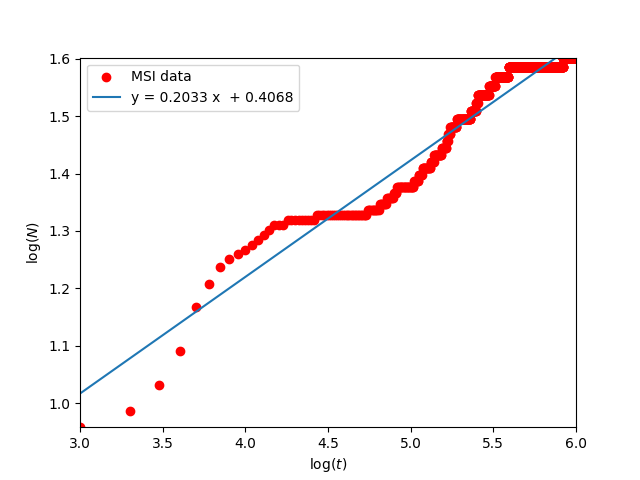
\includegraphics[width=0.4\textwidth]{lw_scaling_p0n2.png}}
        \subfloat[$p = 1$]{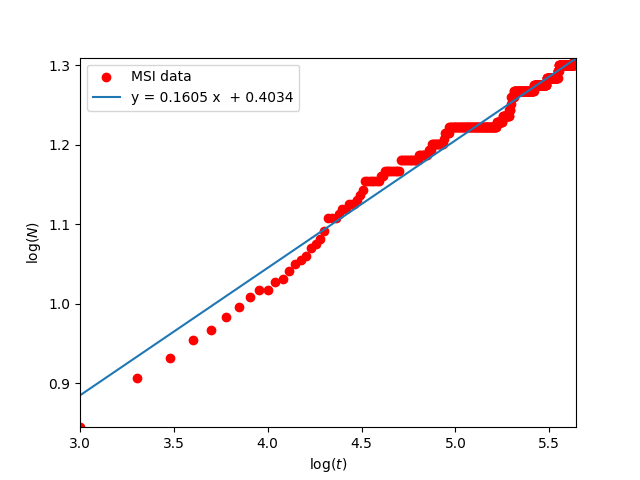
\includegraphics[width=0.4\textwidth]{lw_scaling_p1n2.png}}
    \label{fig:LW_scaling}
\end{figure}
Получените стойности за $\beta = 0.2033; 0.1605$ отговарят именно на очакванията ни на база \autoref{eq:lw_scaling_beta}.

\paragraph{TE} Моделът на \textit{Tersoff} е известно \cite{Krasteva2016}, че има същата времева експонента като този на \textit{Liu \& Weeks}. Провеждайки аналогично изследване с получаване на траектории за $p = 0, 1$ при фиксирано $n =  2$ и последващо определяне на средната брой стъпала в групата $N$ с MSI получаваме зависимостите от \autoref{fig:TE_scaling}. 

Получени са $\beta = 0.2119; 0.1710$ за експонентите от този числен експеримент, което и потвърждава отново очакването за зависимостта $\beta(p)$ да е по \autoref{eq:lw_scaling_beta}.
\begin{figure}[hbpt]
    \centering
    \caption{Скейлингова зависимост на $N(t)$ за \textbf{TE}}
        \subfloat[$p = 0$]{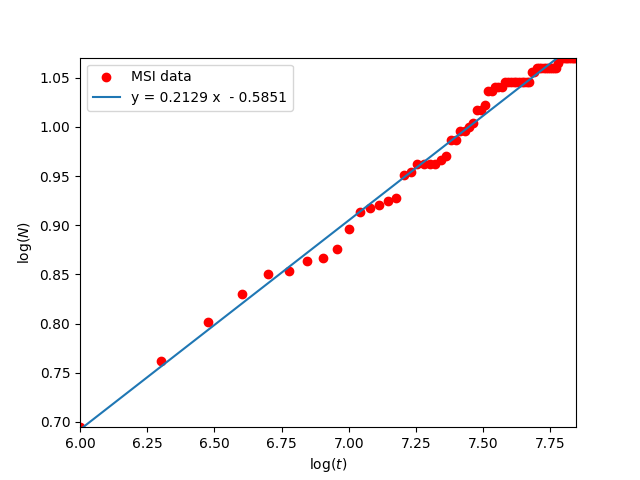
\includegraphics[width=0.4\textwidth]{TE2_scaling_p0n2.png}}
        \subfloat[$p = 1$]{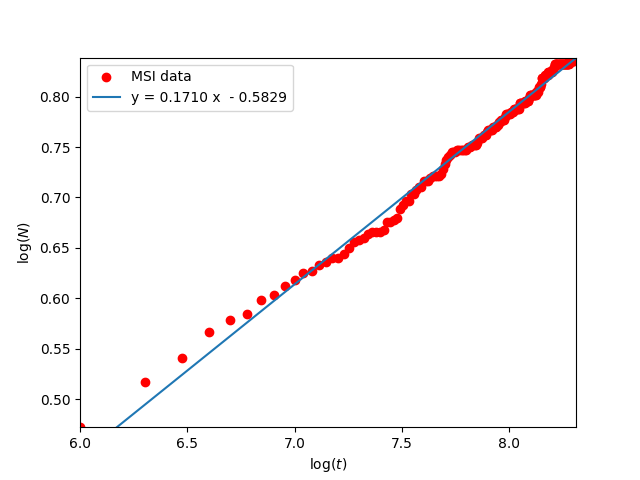
\includegraphics[width=0.4\textwidth]{TE2_scaling_p1n2.png}}
    \label{fig:TE_scaling}
\end{figure}

\paragraph{MM2} Е обстойно изследван като най-прост модел на групиране включително и подробен линеен анализ на устойчивостта на дясната страна  от \textit{Рангелов, Кръстева, Мисбах, Тончев и други} \cite{Ranguelov2012}. Очакваната зависимост за $\beta$ тук е различна:
\begin{equation}
    \beta = \frac{1}{p+3}
    \label{eq:mm_scaling_beta}
\end{equation} 
\begin{figure}[hbpt]
    \centering
    \caption{Скейлингова зависимост на $N(t)$ за \textbf{MM2}}
        \subfloat[$p = 0$]{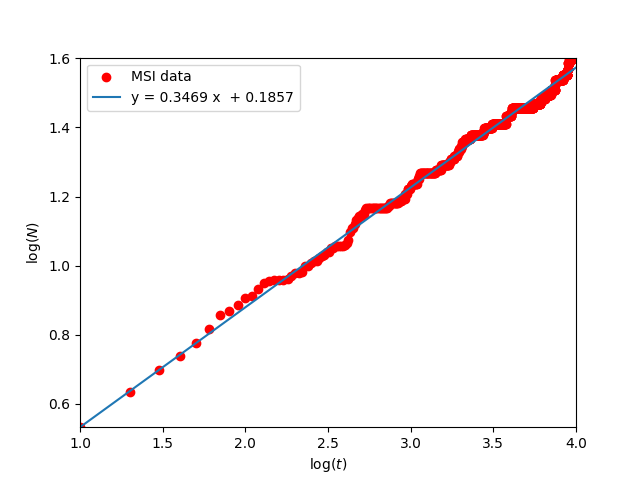
\includegraphics[width=0.4\textwidth]{mm_scaling_p0n2.png}}
        \subfloat[$p = 1$]{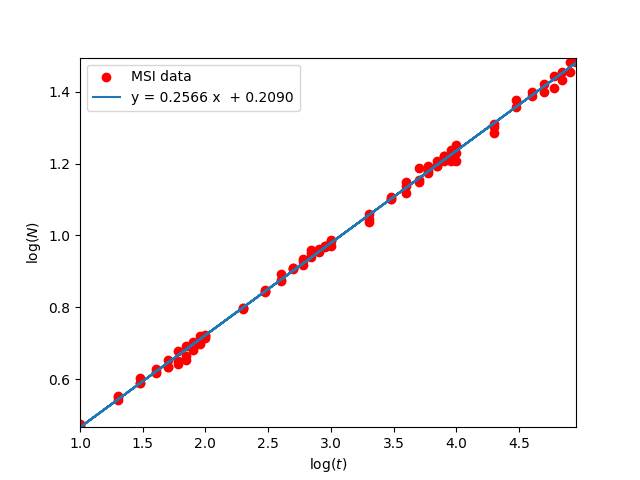
\includegraphics[width=0.4\textwidth]{mm_scaling_p1n2.png}}
    \label{fig:MM_scaling}
\end{figure}

Получаваме за $\beta = 0.3469; 0.2566$ от \autoref{fig:MM_scaling}, което съвпада и с очакванията \autoref{eq:mm_scaling_beta}.

Всеки от тези модели може да бъде изследван за по-голям набор от стойности за $p, n$ и така да се проверят по-пълно зависимостите (и техните отклонения от съответно \autoref{eq:mm_scaling_beta} и \autoref{eq:lw_scaling_beta}). Това представлява и потенциална възможност за бъдещо изследване.

\subsection{Уравнение на PTVV}
\label{par:ptvv}
Уравнението на Pimpinelli-Tonchev-Videcoq-Vladimirova (PTVV) \cite{Pimpinelli2002} \cite{2Krug2005} представлява опит за обобщено описание на феномена групиране (\textbf{B1} и \textbf{B2} тип), особено в специалния случай на прави стъпала. Този модел е по-близо до представата за повърхността показана на \autoref{fig:step_bunching}. Това е нелинейно частно диференциално уравнение от четвърти ред:
\begin{equation}
    \frac{\partial h}{\partial t} + \frac{\partial }{\partial x} \left( K_{1} m^{\rho} + \frac{K_2}{m^k} \frac{\partial^2 }{\partial x^2} m ^ n \right) = 0
    \label{eq:ptvv}
\end{equation}
Където $h$ - локална височина на повърхността в точката $x$, $m \coloneqq \partial h / \partial x$ - локален наклон на повърхността, $K_1, K_2$ са ,,материални константи``, $n$ е експонентата на взаимодействие на разстояние $d$, $U \propto 1/d^n$, като за линейно-еластични стъпала $n = 2$ \cite{Kozlov2022}, $\rho, k$ са кинетични параметри, чиито стойности са обобщени от \textit{Kozlov, et al.} и свързани с морфологичните (скейлинговите) параметри $\alpha, \beta$ в \textit{Табл.~1} на \cite{Kozlov2022}. Задачата се затваря с пертурбирана начална вицинална повърхност с периодични г.у. 

Параметърът $\alpha$ описва съответно скейлинга на \textit{ширината} $W$ на групата с броя стъпала $N$ в нея ($W \propto N^\alpha$), а $\beta$ - времевият скейлинг на броя стъпала в групата ($N \propto t^\beta$).

\textit{Krzyżewski et al.} чрез подробен анализ на размерностите и отношенията на скалите на \autoref{eq:ptvv} \cite{Krzyewski2018} получават експлицитен израз за морфологичния параметър $\alpha$ като функция на параметрите на PTVV-уравнението.
\begin{equation}
    \alpha = \frac{2 - (n-k) - \rho}{(n-k) - \rho}
    \label{eq:alpha_ptvv}
\end{equation}

Целта ни тук ще бъде да получим другия морфологичен параметър $\beta$ чрез изследване на инвариантността под трансформация на разтягане на PTVV. Нека направим преобразованието:
\[\begin{gathered}
  \overline t  = {\varepsilon ^a}t \Leftrightarrow t = {\varepsilon ^{ - a}}\overline t  \\ 
  \overline x  = {\varepsilon ^b}x \Leftrightarrow x = {\varepsilon ^{ - b}}\overline x  \\ 
  \overline h  = {\varepsilon ^c}h \Leftrightarrow h = {\varepsilon ^{ - c}}\overline h
\end{gathered} \]
Нека отбележим решението на разглежданата и трансформираната задача съответно с (2D равнина):
\begin{align*}
    h  &= \phi(x, t) \\
    \overline{h} &= \overline{\phi}(\overline{x}, \overline{t})
\end{align*}
Очевидно е, че ако $h  = \phi(x, t)$ e решение на горното ЧДУ, то $\overline{h} = \overline{\phi}(\overline{x}, \overline{t})$ е решение на:
\begin{equation*}
    \frac{\partial \overline h}{\partial \overline t} + \frac{\partial }{\partial \overline x} \left( K_{1} \overline m^{\rho} + \frac{K_2}{\overline m^k} \frac{\partial^2 }{\partial \overline x^2} \overline m ^ n \right) = 0
\end{equation*}
Заместваме трансформираните променливи в основното уравнение и извършваме преобразованията:
\begin{equation*}
    {\varepsilon ^{a - c}}\frac{{\partial \overline h }}{{\partial \overline t }} + {\varepsilon ^b}\frac{\partial }{{\partial \overline x }}\left( {{K_1}{{\left( {{\varepsilon ^{b - c}}\frac{{\partial \overline h }}{{\partial \overline x }}} \right)}^\rho } + \frac{{{K_2}}}{{{{\left( {{\varepsilon ^{b - c}}\frac{{\partial \overline h }}{{\partial \overline x }}} \right)}^k}}}{\varepsilon ^{2b}}\frac{{{\partial ^2}}}{{\partial {{\overline x }^2}}}{{\left( {{\varepsilon ^{b - c}}\frac{{\partial \overline h }}{{\partial \overline x }}} \right)}^n}} \right) = 0
\end{equation*}
\begin{equation}
   {\varepsilon ^{a - c}}\frac{{\partial \overline h }}{{\partial \overline t }} + \frac{\partial }{{\partial \overline x }}\left( {{\varepsilon ^{b + \rho (b - c)}}{K_1}{{\left( {\frac{{\partial \overline h }}{{\partial \overline x }}} \right)}^\rho } + {\varepsilon ^{b - k(b - c) + 2b + n(b - c)}}\frac{{{K_2}}}{{{{\left( {\frac{{\partial \overline h }}{{\partial \overline x }}} \right)}^k}}}\frac{{{\partial ^2}}}{{\partial {{\overline x }^2}}}{{\left( {\frac{{\partial \overline h }}{{\partial \overline x }}} \right)}^n}} \right) = 0
   \label{eq:ptvv_subst_eps}
\end{equation}

\begin{definition}{Инвариантност под разтягане}{stretching_transform}
    ЧДУ е инвариантно (с точност до константа) относно семейството на трансформации на разтягане, ако е в сила:
    \begin{equation*}
        \label{eq:stretching_transform}
        F(x,t,h,{h_t},{h_x},{h_{xx}},{h_{xxx}},{h_{xxxx}}) = A(\varepsilon )F(\overline x ,\overline t ,\overline h ,\overline h \overline {_t} ,{\overline h _{\overline x }},{\overline h _{\overline {xx} }},{\overline h _{\overline {xxx} }},{\overline h _{\overline {xxxx} }})
    \end{equation*}
    За всяко  $\varepsilon$, за някаква $A(\varepsilon)$, такава че $A(1) = 1$. Ако $A(\varepsilon) \equiv 1$, то уравнението е абсолютно инвариантно.
\end{definition}
Тогава от \autoref{def:stretching_transform} директно следва, че ако разглежданото уравнение е инвариантно под трансформацията на разтягане, то $\overline{h} = \overline{\phi}(\overline{x}, \overline{t})$ ще е решение и на оригиналното уравнение.
\begin{definition}{Инвариантни решения}{invariant_solution}
    Едно решение е инвариантно относно трансформацията на разтягане, ако е в сила:
    \begin{equation*}
        \label{eq:invariant_equation}
        \phi (\overline x ,\overline t ) = \overline \phi  (\overline x ,\overline t )
    \end{equation*}
    Автомоделните решения от вида $\phi  = \omega (t)f(s(x,t))$, където $\omega(t)$ - „амплитуда“,  $f(s(x,t))$- автомоделна функция,  $s(x,t)$ - автомоделна променлива са измежду инвариантните на разтягане решения.
\end{definition}
\noindent За да отговаря на \autoref{def:stretching_transform}, за \autoref{eq:ptvv_subst_eps} тогава е необходимо да е изпълнено:
\begin{equation*}
    a - c = b + (b - c)\rho  = c(k - n) + b(3 - k + n)
\end{equation*}
Решаваме системата за $a, c$:
\begin{align*}
    a &= \frac{{2\left( {k - n + 2\rho  - 1} \right)}}{{k - n + \rho }}b \\
    c &= \left( {1 - \frac{2}{{k - n + \rho }}} \right)b
\end{align*}
Тогава от \autoref{def:invariant_solution} имаме:
\begin{equation*}
    \phi ({\varepsilon ^b}x,{\varepsilon ^a}t) = {\varepsilon ^c}\phi (x,t)
\end{equation*}
Диференцираме по $\varepsilon$ и слагаме $\varepsilon = 1$, като получаваме следното ОДУ:
\begin{equation*}
    b x{\phi _x} + a t{\phi _t} = c \phi
\end{equation*}
Това уравнение има известно общо аналитично решение във вида:
\begin{equation*}
    \phi(x, t) = t^{c/a} f \left(x^a / t^b \right)
\end{equation*}
Ще изберем частния случай на $b = 1$ и ще положим:
\begin{align*}
    q & \coloneqq c/a = \frac{{k - n + \rho  - 2}}{{2\left( { - 1 + k - n + 2\rho } \right)}} \\
    p & \coloneqq a= \frac{{2\left( {k - n + 2\rho  - 1} \right)}}{{k - n + \rho }} \\
    s & \coloneqq \frac{x^p}{t}
\end{align*}
Тогава, замествайки полаганията получаваме:
\begin{equation*}
    h = \phi(x, t) = t^q f(s)
\end{equation*}
Това ни позволява да пресметнем за ,,каноничните`` стойности на $k, \rho$ от PTVV \cite{Kozlov2022} параметъра $q$:
\begin{table}[hbpt]
\centering
\caption{Стойности на $q$ за различни стойности на $k, \rho$}
\resizebox{0.3\linewidth}{!}{%
\begin{tabular}{cccc} 
\toprule
\multicolumn{1}{l}{\diagbox{$k$}{$\rho$}} & \multicolumn{1}{l}{$-1$} & \multicolumn{1}{l}{$0$}                      & $1$        \\ 
\hline
$0$                                       & $1/2$                    & $2/3$                                        & $3/2$      \\ 
\hline
$1$                                       & $1/2$                    & $3/4$                                        & $\infty $  \\ 
\hline
$2$                                       & $1/2$                    & -                                            & $-1/2$     \\
\bottomrule
\end{tabular}
}
\label{tabl:q_param}
\end{table}
Ако сравним \autoref{tabl:q_param} с \textit{Табл.~1} от \cite{Kozlov2022}, виждаме че това са именно стойностите на параметъра $\beta$, т.е. $\beta = q$. Нещо повече - знаем че броят стъпала в групата $N$ в даден момент е пропорционален на $t^\beta$. Тогава ако сравним:
\begin{align*}
    N      & \propto t^\beta \\
    h/f(s) & \propto t^\beta 
\end{align*}
Или $N \propto h/f(s)$, т.е. броят стъпала в групата е пропорционален на височината на повърхността, разделена на автомоделната функция. Този резултат е естествен и съвпада с очакванията височината да зависи от броя стъпала в дадена група. В \cite{Kozlov2022} стойностите за $\beta$ са получени от анализ на размерностите на частни случаи или от числени експерименти, а тук получихме директната връзка между параметрите на модела:
\begin{result}{Израз за морфологичния параметър $\beta$}{beta_rho_k_n_rel}
    \begin{equation}
        \beta = \frac{{k - n + \rho  - 2}}{{2\left( { - 1 + k - n + 2\rho } \right)}}
        \label{eq:beta_explicit}
    \end{equation}
\end{result}

Теорията на инвариантните под разтягане решения също така показва, че ако заместим автомоделното решение в основното ЧДУ, то може да бъде сведено до ОДУ за автомоделната функция $f(s)$ по отношение на автомоделната променлива $s$. За общия вид $h  = t^q f(s)$ не е получено обобщено ОДУ, но например за конкретния избор на  $k = 2, \rho  = 1, n = 2$ заместваме автомоделното решение и съкращаваме на $t^q$, получаваме следното ОДУ:
\[\begin{gathered}
  16{K_2}{s^2}\left( { - 3{{\left( {s{f^{(2)}}} \right)}^2} + 2s\left( {{f^{(3)}}s} \right)\left( {s{f^{(2)}}} \right) + \left( {2s\left( {{f^{(4)}}s} \right) + 7{f^{(3)}}s} \right)\left( {s{f^{(1)}}} \right)} \right) =  \hfill \\
   = 2{s^{3/2}}\left( {s - 2{K_1}} \right){\left( {s{f^{(1)}}} \right)^3} + {\left( {s{f^{(1)}}} \right)^2}\left( { - 8{K_1}{s^{5/2}}\left( {s{f^{(2)}}} \right) + {s^{3/2}}(fs) + 8{K_2}} \right) + \frac{{64{K_2}{s^3}{{\left( {s{f^{(2)}}} \right)}^3}}}{{s{f^{(1)}}}} \hfill \\ 
\end{gathered} \]
Това e \textit{нелинейно} ОДУ от 4 ред и заедно с периодичните г.у. представлява гранична задача. Численото му решение изисква специално третиране, тъй като трябва да се прескалира началната вицинала по съответен начин. Освен това тази гранична задача трябва да бъде превърната в начална, която може да бъде решена числено със стандарти методи за интегриране на задачи на Коши. Това може да постигнато с т.нар. метод на прострелката (\textit{shooting method}). В тази посока \textit{Guedda, et al.} \cite{Guedda2022} са изследвали уравнението на \textit{Golubović}, което е по-обща форма на PTVV изведена за друг контекст. Те са получили числени решения за автомоделната функция $f(s)$ (макар и само в контекста на \textit{анзаца} на \textit{Family-Viscek}) и това може да бъде оправна точка за бъдещи разработки по численото решаване на PTVV.

\subsection{Уравнение на Стоянов-Тончев (ST)}
Уравнението на Стоянов-Тончев също е уравнение за групиране на стъпала получено през 1998~г \cite{StoyanovTonchev}. В перспектива, то представлява частен случай на PTVV, който описва специфичен режим на групиране. В него отново е основно предположението за отблъскване между стъпалата на разстояние $d$ зададено от закона $U = A/d^2$, където $A = const$ e магнитудът на отблъскване:
\begin{equation}
    \label{eq:stoyanov_tonchev_dimensional}
    \frac{\partial h}{\partial t} = B \left[ - \frac{6 a^2 A}{h^2_0} \frac{\partial^2}{\partial x^2} \left( \frac{\partial h}{\partial x} \frac{\partial^2 h}{\partial x^2}  \right) + 2 F \frac{b}{h_0} \left( \frac{\partial^2 h}{\partial x^2}  \right) \right] 
\end{equation}
Където $a$, $h_0$ са ,,атомните мащаби`` за $x$, $h$, $B = \frac{D_s n^e_s}{k \Theta} \Omega$ е материален параметър характеризиращ дифузията на адатомите, $F$ - силата на електромиграцията.

Ще започнем с обезразмеряването на уравнението, като приложим същият ,,трик`` като при обобщения ОДУ-модел с избор на скалите, така че в обезразмереното уравнение да няма явни параметри. Избираме $H \coloneqq h/\xi_y$, $X \coloneqq x/\xi_x$ и $T \coloneqq t/\tau$. Заместваме в \autoref{eq:stoyanov_tonchev_dimensional} заедно с експлицитния вид на всички параметри и получаваме:
\begin{equation*}
\frac{{\partial H}}{{\partial T}} =  - \frac{{{D_s}n_s^e}}{{k\Theta }}\Omega \frac{{6abA\tau {\xi _y}}}{{\xi _x^5h_0^2}}\frac{{{\partial ^2}}}{{\partial {X^2}}}\left( {\frac{{\partial H}}{{\partial X}}\frac{{{\partial ^2}H}}{{\partial {X^2}}}} \right) + \frac{{{D_s}n_s^e}}{{k\Theta }}\Omega \frac{{2Fb\tau }}{{\xi _x^2{h_0}}}\left( {\frac{{{\partial ^2}H}}{{\partial {X^2}}}} \right)
\end{equation*}
Получаваме система от две уравнения за три неизвестни:
\begin{equation}
    \label{eq:stoyanov_tonchev_scales_system}
    \begin{cases}
        \frac{{{D_s}n_s^e}}{{k\Theta }}\frac{{6abA}}{{h_0^2}}\Omega \frac{{\tau {\xi _y}}}{{\xi _x^5}} = 1 \\
        \frac{{{D_s}n_s^e}}{{k\Theta }}\frac{{2Fb}}{{{h_0}}}\Omega \frac{\tau }{{\xi _x^2}} = 1
    \end{cases} 
\end{equation}
и обезразмерената форма на ST:
\begin{equation}
    \label{eq:stoyanov_tonchev_dimensionless}
    \frac{\partial H}{\partial T} = - \frac{\partial^2}{\partial X^2} \left( \frac{\partial H}{\partial X} \frac{\partial^2 H}{\partial X^2} \right) + \left( \frac{\partial^2 H}{\partial X^2} \right)
\end{equation}
Тогава можем да получим по-удобните връзки между скалите:
\begin{align*}
    \tau  = \frac{{k\Theta {h_0}}}{{2\Omega Fb{D_s}n_s^e}}\xi _x^2 \\
    {\xi _x} = {\left( {\frac{{3aA}}{{F{h_0}}}{\xi _y}} \right)^{1/3}}
\end{align*}
И можем условно да поставим, че големината на групата (броят стъпала $N$) е $N \coloneqq \xi_y / h_0$ (характеристична височина разделена на ,,кванта`` височина). Така получаваме междинно:
\begin{equation*}
    \xi_x = \left( \frac{3 a A}{F}  N \right) ^ {1/3}
\end{equation*}
Тогава ако разделим $\xi_{x}$ на броя стъпала $N$, ще получим оценка за средната \textit{ширина} на групата $\langle l\rangle_b$:
\begin{equation*}
    {\left\langle l \right\rangle _b} \coloneqq \frac{{{\xi _x}}}{N} = {\left( {\frac{{3aA}}{{F{N^2}}}} \right)^{1/3}}
\end{equation*}
Можем да сравним с оригиналния труд на Стоянов и Тончев \cite{StoyanovTonchev}, където е получена връзката:
\begin{equation*}
    {\left\langle l \right\rangle _b} = 1.563{\left( {\frac{{3aA}}{{\left| F \right|{N^2}}}} \right)^{1/3}}
\end{equation*}
чрез интегриране на \autoref{eq:stoyanov_tonchev_dimensional} при съответни приближения.

Получаването на \autoref{eq:stoyanov_tonchev_dimensionless} значително опростява работата с него и затова ще изследваме неговата инвариантност под трансформация на разтягане, аналогично на PTVV. Ще използваме същата нотация за трансформираните променливи като в \autoref{par:ptvv} и директно ще заместим в \autoref{eq:stoyanov_tonchev_dimensionless}, като отново само ще разгледаме основното ЧДУ, което ще сведем до ОДУ за автомоделната функция $f(s)$, без да го решаваме:
\begin{align*}
    {\varepsilon ^{a - c}}\frac{{\partial \bar H}}{{\partial \bar T}} &=  - {\varepsilon ^{2b}}\frac{\partial }{{\partial {{\bar X}^2}}}\left( {{\varepsilon ^{b - c}}\frac{{\partial \bar H}}{{\partial \bar X}}{\varepsilon ^{2b - c}}\frac{{{\partial ^2}\bar H}}{{\partial {{\bar X}^2}}}} \right) + {\varepsilon ^{2b - c}}\frac{{{\partial ^2}\bar H}}{{\partial {{\bar X}^2}}} \\
    {\varepsilon ^{a - c}}\frac{{\partial \bar H}}{{\partial \bar T}} &=  - {\varepsilon ^{5b - 2c}}\frac{\partial }{{\partial \bar X}}\left( {\frac{{\partial \bar H}}{{\partial \bar X}}\frac{{{\partial ^2}\bar H}}{{\partial {{\bar X}^2}}}} \right) + {\varepsilon ^{2b - c}}\frac{{{\partial ^2}\bar H}}{{\partial {{\bar X}^2}}}
\end{align*}
Така получаваме системата за параметрите $a, b, c$:
\begin{equation*}
    a - c = 5b - 2c = 2b - c
\end{equation*}
И съответно:
\begin{equation}
    \begin{cases}
        b = \frac{a}{2} \\
        c = \frac{3}{2} a
    \end{cases} 
\end{equation}
Тогава семейството инвариантни решения (при вариране на параметъра $a$) има общия вид:
\begin{equation}
        h = \phi (x,t) = {t^{c/a}}f\left( {\frac{{{x^a}}}{{{t^b}}}} \right) = {t^{3/2}}f\left( {\frac{{{x^a}}}{{{t^{a/2}}}}} \right)
\end{equation}
Тогава, времевият скейлинг на ST ($N \propto t^\beta$) можем да дадем като:
\begin{equation}
    N \propto \frac{h(x,t)}{f(s)} = t^{3/2}
\end{equation}
Обратно, можем да изследваме поведението $h/t^{3/2}$ и така при правилно построена процедура за параметрична идентификация да определим конкретната стойност на $a$ в автомоделната променлива $s_a(x,t) = x^a/t^{a/2}$. Ако изберем $a = 1$ и заместим анзаца в \autoref{eq:stoyanov_tonchev_dimensionless}:
\begin{result}{Анзац на Family-Vicsek за ST}{st_family_viscek}
    \begin{equation*}
        h(x,t) = {t^{3/2}}f\left( {\frac{{{x}}}{{{\sqrt{t}}}}} \right)
    \end{equation*}
\end{result}
\noindent Отново получаваме ОДУ за автомоделната функция $f(s)$, където $s \coloneqq x/\sqrt{t}$:
\begin{align*}
    \sqrt t \left( { - \left( {s - 2{f^{(4)}}(s)} \right)f'(s) + 2\left( {3{f^{(3)}}(s) - 1} \right)f''(s) + 3f(s)} \right) = 0 \\
     2\left( {3{f^{(3)}}(s) - 1} \right)f''(s) + 3f(s) = \left( {s - 2{f^{(4)}}(s)} \right)f'(s), \quad t \ne 0 \\
\end{align*}
Пред решаването на това ОДУ стоят същите проблеми като при PTVV, основно свързани с особените начални и гранични условия на системата. Въпреки това този резултат е полезен, защото директно показва кой частен случай на PTVV е ST и дава възможност за широки изследвания за междинната асимптотика на това семейство модели.